\documentclass{puthesis}

\RequirePackage[round]{natbib}

\bibliographystyle{plainnat}

% Recommended, but optional, packages for figures and better typesetting:
\usepackage{microtype}
\usepackage{graphicx}
% \usepackage{subfigure}
\usepackage{booktabs} % for professional tables
\usepackage{paralist}
\usepackage{enumitem}
\usepackage{adjustbox}
\usepackage{sidecap}
\usepackage{wrapfig}

\usepackage{caption}
\usepackage{subcaption}
% \usepackage[backend=bibtex]{biblatex}

\usepackage[ruled,vlined]{algorithm2e}

\usepackage{import}

\usepackage[utf8]{inputenc} % allow utf-8 input
\usepackage[T1]{fontenc}    % use 8-bit T1 fonts
\usepackage{url}

%%%%% NEW MATH DEFINITIONS %%%%%

\usepackage{amsmath,amsfonts,bm}

% Mark sections of captions for referring to divisions of figures
\newcommand{\figleft}{{\em (Left)}}
\newcommand{\figcenter}{{\em (Center)}}
\newcommand{\figright}{{\em (Right)}}
\newcommand{\figtop}{{\em (Top)}}
\newcommand{\figbottom}{{\em (Bottom)}}
\newcommand{\captiona}{{\em (a)}}
\newcommand{\captionb}{{\em (b)}}
\newcommand{\captionc}{{\em (c)}}
\newcommand{\captiond}{{\em (d)}}

% Highlight a newly defined term
\newcommand{\newterm}[1]{{\bf #1}}


% Figure reference, lower-case.
\def\figref#1{figure~\ref{#1}}
% Figure reference, capital. For start of sentence
\def\Figref#1{Figure~\ref{#1}}
\def\twofigref#1#2{figures \ref{#1} and \ref{#2}}
\def\quadfigref#1#2#3#4{figures \ref{#1}, \ref{#2}, \ref{#3} and \ref{#4}}
% Section reference, lower-case.
\def\secref#1{section~\ref{#1}}
% Section reference, capital.
\def\Secref#1{Section~\ref{#1}}
% Reference to two sections.
\def\twosecrefs#1#2{sections \ref{#1} and \ref{#2}}
% Reference to three sections.
\def\secrefs#1#2#3{sections \ref{#1}, \ref{#2} and \ref{#3}}
% Reference to an equation, lower-case.
\def\eqref#1{equation~\ref{#1}}
% Reference to an equation, upper case
\def\Eqref#1{Equation~\ref{#1}}
% A raw reference to an equation---avoid using if possible
\def\plaineqref#1{\ref{#1}}
% Reference to a chapter, lower-case.
\def\chapref#1{chapter~\ref{#1}}
% Reference to an equation, upper case.
\def\Chapref#1{Chapter~\ref{#1}}
% Reference to a range of chapters
\def\rangechapref#1#2{chapters\ref{#1}--\ref{#2}}
% Reference to an algorithm, lower-case.
\def\algref#1{algorithm~\ref{#1}}
% Reference to an algorithm, upper case.
\def\Algref#1{Algorithm~\ref{#1}}
\def\twoalgref#1#2{algorithms \ref{#1} and \ref{#2}}
\def\Twoalgref#1#2{Algorithms \ref{#1} and \ref{#2}}
% Reference to a part, lower case
\def\partref#1{part~\ref{#1}}
% Reference to a part, upper case
\def\Partref#1{Part~\ref{#1}}
\def\twopartref#1#2{parts \ref{#1} and \ref{#2}}

\def\ceil#1{\lceil #1 \rceil}
\def\floor#1{\lfloor #1 \rfloor}
\def\1{\bm{1}}
\newcommand{\train}{\mathcal{D}}
\newcommand{\valid}{\mathcal{D_{\mathrm{valid}}}}
\newcommand{\test}{\mathcal{D_{\mathrm{test}}}}

\def\eps{{\epsilon}}


% Random variables
\def\reta{{\textnormal{$\eta$}}}
\def\ra{{\textnormal{a}}}
\def\rb{{\textnormal{b}}}
\def\rc{{\textnormal{c}}}
\def\rd{{\textnormal{d}}}
\def\re{{\textnormal{e}}}
\def\rf{{\textnormal{f}}}
\def\rg{{\textnormal{g}}}
\def\rh{{\textnormal{h}}}
\def\ri{{\textnormal{i}}}
\def\rj{{\textnormal{j}}}
\def\rk{{\textnormal{k}}}
\def\rl{{\textnormal{l}}}
% rm is already a command, just don't name any random variables m
\def\rn{{\textnormal{n}}}
\def\ro{{\textnormal{o}}}
\def\rp{{\textnormal{p}}}
\def\rq{{\textnormal{q}}}
\def\rr{{\textnormal{r}}}
\def\rs{{\textnormal{s}}}
\def\rt{{\textnormal{t}}}
\def\ru{{\textnormal{u}}}
\def\rv{{\textnormal{v}}}
\def\rw{{\textnormal{w}}}
\def\rx{{\textnormal{x}}}
\def\ry{{\textnormal{y}}}
\def\rz{{\textnormal{z}}}

% Random vectors
\def\rvepsilon{{\mathbf{\epsilon}}}
\def\rvtheta{{\mathbf{\theta}}}
\def\rva{{\mathbf{a}}}
\def\rvb{{\mathbf{b}}}
\def\rvc{{\mathbf{c}}}
\def\rvd{{\mathbf{d}}}
\def\rve{{\mathbf{e}}}
\def\rvf{{\mathbf{f}}}
\def\rvg{{\mathbf{g}}}
\def\rvh{{\mathbf{h}}}
\def\rvu{{\mathbf{i}}}
\def\rvj{{\mathbf{j}}}
\def\rvk{{\mathbf{k}}}
\def\rvl{{\mathbf{l}}}
\def\rvm{{\mathbf{m}}}
\def\rvn{{\mathbf{n}}}
\def\rvo{{\mathbf{o}}}
\def\rvp{{\mathbf{p}}}
\def\rvq{{\mathbf{q}}}
\def\rvr{{\mathbf{r}}}
\def\rvs{{\mathbf{s}}}
\def\rvt{{\mathbf{t}}}
\def\rvu{{\mathbf{u}}}
\def\rvv{{\mathbf{v}}}
\def\rvw{{\mathbf{w}}}
\def\rvx{{\mathbf{x}}}
\def\rvy{{\mathbf{y}}}
\def\rvz{{\mathbf{z}}}

% Elements of random vectors
\def\erva{{\textnormal{a}}}
\def\ervb{{\textnormal{b}}}
\def\ervc{{\textnormal{c}}}
\def\ervd{{\textnormal{d}}}
\def\erve{{\textnormal{e}}}
\def\ervf{{\textnormal{f}}}
\def\ervg{{\textnormal{g}}}
\def\ervh{{\textnormal{h}}}
\def\ervi{{\textnormal{i}}}
\def\ervj{{\textnormal{j}}}
\def\ervk{{\textnormal{k}}}
\def\ervl{{\textnormal{l}}}
\def\ervm{{\textnormal{m}}}
\def\ervn{{\textnormal{n}}}
\def\ervo{{\textnormal{o}}}
\def\ervp{{\textnormal{p}}}
\def\ervq{{\textnormal{q}}}
\def\ervr{{\textnormal{r}}}
\def\ervs{{\textnormal{s}}}
\def\ervt{{\textnormal{t}}}
\def\ervu{{\textnormal{u}}}
\def\ervv{{\textnormal{v}}}
\def\ervw{{\textnormal{w}}}
\def\ervx{{\textnormal{x}}}
\def\ervy{{\textnormal{y}}}
\def\ervz{{\textnormal{z}}}

% Random matrices
\def\rmA{{\mathbf{A}}}
\def\rmB{{\mathbf{B}}}
\def\rmC{{\mathbf{C}}}
\def\rmD{{\mathbf{D}}}
\def\rmE{{\mathbf{E}}}
\def\rmF{{\mathbf{F}}}
\def\rmG{{\mathbf{G}}}
\def\rmH{{\mathbf{H}}}
\def\rmI{{\mathbf{I}}}
\def\rmJ{{\mathbf{J}}}
\def\rmK{{\mathbf{K}}}
\def\rmL{{\mathbf{L}}}
\def\rmM{{\mathbf{M}}}
\def\rmN{{\mathbf{N}}}
\def\rmO{{\mathbf{O}}}
\def\rmP{{\mathbf{P}}}
\def\rmQ{{\mathbf{Q}}}
\def\rmR{{\mathbf{R}}}
\def\rmS{{\mathbf{S}}}
\def\rmT{{\mathbf{T}}}
\def\rmU{{\mathbf{U}}}
\def\rmV{{\mathbf{V}}}
\def\rmW{{\mathbf{W}}}
\def\rmX{{\mathbf{X}}}
\def\rmY{{\mathbf{Y}}}
\def\rmZ{{\mathbf{Z}}}

% Elements of random matrices
\def\ermA{{\textnormal{A}}}
\def\ermB{{\textnormal{B}}}
\def\ermC{{\textnormal{C}}}
\def\ermD{{\textnormal{D}}}
\def\ermE{{\textnormal{E}}}
\def\ermF{{\textnormal{F}}}
\def\ermG{{\textnormal{G}}}
\def\ermH{{\textnormal{H}}}
\def\ermI{{\textnormal{I}}}
\def\ermJ{{\textnormal{J}}}
\def\ermK{{\textnormal{K}}}
\def\ermL{{\textnormal{L}}}
\def\ermM{{\textnormal{M}}}
\def\ermN{{\textnormal{N}}}
\def\ermO{{\textnormal{O}}}
\def\ermP{{\textnormal{P}}}
\def\ermQ{{\textnormal{Q}}}
\def\ermR{{\textnormal{R}}}
\def\ermS{{\textnormal{S}}}
\def\ermT{{\textnormal{T}}}
\def\ermU{{\textnormal{U}}}
\def\ermV{{\textnormal{V}}}
\def\ermW{{\textnormal{W}}}
\def\ermX{{\textnormal{X}}}
\def\ermY{{\textnormal{Y}}}
\def\ermZ{{\textnormal{Z}}}

% Vectors
\def\vzero{{\bm{0}}}
\def\vone{{\bm{1}}}
\def\vmu{{\bm{\mu}}}
\def\vtheta{{\bm{\theta}}}
\def\va{{\bm{a}}}
\def\vb{{\bm{b}}}
\def\vc{{\bm{c}}}
\def\vd{{\bm{d}}}
\def\ve{{\bm{e}}}
\def\vf{{\bm{f}}}
\def\vg{{\bm{g}}}
\def\vh{{\bm{h}}}
\def\vi{{\bm{i}}}
\def\vj{{\bm{j}}}
\def\vk{{\bm{k}}}
\def\vl{{\bm{l}}}
\def\vm{{\bm{m}}}
\def\vn{{\bm{n}}}
\def\vo{{\bm{o}}}
\def\vp{{\bm{p}}}
\def\vq{{\bm{q}}}
\def\vr{{\bm{r}}}
\def\vs{{\bm{s}}}
\def\vt{{\bm{t}}}
\def\vu{{\bm{u}}}
\def\vv{{\bm{v}}}
\def\vw{{\bm{w}}}
\def\vx{{\bm{x}}}
\def\vy{{\bm{y}}}
\def\vz{{\bm{z}}}

% Elements of vectors
\def\evalpha{{\alpha}}
\def\evbeta{{\beta}}
\def\evepsilon{{\epsilon}}
\def\evlambda{{\lambda}}
\def\evomega{{\omega}}
\def\evmu{{\mu}}
\def\evpsi{{\psi}}
\def\evsigma{{\sigma}}
\def\evtheta{{\theta}}
\def\eva{{a}}
\def\evb{{b}}
\def\evc{{c}}
\def\evd{{d}}
\def\eve{{e}}
\def\evf{{f}}
\def\evg{{g}}
\def\evh{{h}}
\def\evi{{i}}
\def\evj{{j}}
\def\evk{{k}}
\def\evl{{l}}
\def\evm{{m}}
\def\evn{{n}}
\def\evo{{o}}
\def\evp{{p}}
\def\evq{{q}}
\def\evr{{r}}
\def\evs{{s}}
\def\evt{{t}}
\def\evu{{u}}
\def\evv{{v}}
\def\evw{{w}}
\def\evx{{x}}
\def\evy{{y}}
\def\evz{{z}}

% Matrix
\def\mA{{\bm{A}}}
\def\mB{{\bm{B}}}
\def\mC{{\bm{C}}}
\def\mD{{\bm{D}}}
\def\mE{{\bm{E}}}
\def\mF{{\bm{F}}}
\def\mG{{\bm{G}}}
\def\mH{{\bm{H}}}
\def\mI{{\bm{I}}}
\def\mJ{{\bm{J}}}
\def\mK{{\bm{K}}}
\def\mL{{\bm{L}}}
\def\mM{{\bm{M}}}
\def\mN{{\bm{N}}}
\def\mO{{\bm{O}}}
\def\mP{{\bm{P}}}
\def\mQ{{\bm{Q}}}
\def\mR{{\bm{R}}}
\def\mS{{\bm{S}}}
\def\mT{{\bm{T}}}
\def\mU{{\bm{U}}}
\def\mV{{\bm{V}}}
\def\mW{{\bm{W}}}
\def\mX{{\bm{X}}}
\def\mY{{\bm{Y}}}
\def\mZ{{\bm{Z}}}
\def\mBeta{{\bm{\beta}}}
\def\mPhi{{\bm{\Phi}}}
\def\mLambda{{\bm{\Lambda}}}
\def\mSigma{{\bm{\Sigma}}}

% Tensor
\DeclareMathAlphabet{\mathsfit}{\encodingdefault}{\sfdefault}{m}{sl}
\SetMathAlphabet{\mathsfit}{bold}{\encodingdefault}{\sfdefault}{bx}{n}
\newcommand{\tens}[1]{\bm{\mathsfit{#1}}}
\def\tA{{\tens{A}}}
\def\tB{{\tens{B}}}
\def\tC{{\tens{C}}}
\def\tD{{\tens{D}}}
\def\tE{{\tens{E}}}
\def\tF{{\tens{F}}}
\def\tG{{\tens{G}}}
\def\tH{{\tens{H}}}
\def\tI{{\tens{I}}}
\def\tJ{{\tens{J}}}
\def\tK{{\tens{K}}}
\def\tL{{\tens{L}}}
\def\tM{{\tens{M}}}
\def\tN{{\tens{N}}}
\def\tO{{\tens{O}}}
\def\tP{{\tens{P}}}
\def\tQ{{\tens{Q}}}
\def\tR{{\tens{R}}}
\def\tS{{\tens{S}}}
\def\tT{{\tens{T}}}
\def\tU{{\tens{U}}}
\def\tV{{\tens{V}}}
\def\tW{{\tens{W}}}
\def\tX{{\tens{X}}}
\def\tY{{\tens{Y}}}
\def\tZ{{\tens{Z}}}


% Graph
\def\gA{{\mathcal{A}}}
\def\gB{{\mathcal{B}}}
\def\gC{{\mathcal{C}}}
\def\gD{{\mathcal{D}}}
\def\gE{{\mathcal{E}}}
\def\gF{{\mathcal{F}}}
\def\gG{{\mathcal{G}}}
\def\gH{{\mathcal{H}}}
\def\gI{{\mathcal{I}}}
\def\gJ{{\mathcal{J}}}
\def\gK{{\mathcal{K}}}
\def\gL{{\mathcal{L}}}
\def\gM{{\mathcal{M}}}
\def\gN{{\mathcal{N}}}
\def\gO{{\mathcal{O}}}
\def\gP{{\mathcal{P}}}
\def\gQ{{\mathcal{Q}}}
\def\gR{{\mathcal{R}}}
\def\gS{{\mathcal{S}}}
\def\gT{{\mathcal{T}}}
\def\gU{{\mathcal{U}}}
\def\gV{{\mathcal{V}}}
\def\gW{{\mathcal{W}}}
\def\gX{{\mathcal{X}}}
\def\gY{{\mathcal{Y}}}
\def\gZ{{\mathcal{Z}}}

% Sets
\def\sA{{\mathbb{A}}}
\def\sB{{\mathbb{B}}}
\def\sC{{\mathbb{C}}}
\def\sD{{\mathbb{D}}}
% Don't use a set called E, because this would be the same as our symbol
% for expectation.
\def\sF{{\mathbb{F}}}
\def\sG{{\mathbb{G}}}
\def\sH{{\mathbb{H}}}
\def\sI{{\mathbb{I}}}
\def\sJ{{\mathbb{J}}}
\def\sK{{\mathbb{K}}}
\def\sL{{\mathbb{L}}}
\def\sM{{\mathbb{M}}}
\def\sN{{\mathbb{N}}}
\def\sO{{\mathbb{O}}}
\def\sP{{\mathbb{P}}}
\def\sQ{{\mathbb{Q}}}
\def\sR{{\mathbb{R}}}
\def\sS{{\mathbb{S}}}
\def\sT{{\mathbb{T}}}
\def\sU{{\mathbb{U}}}
\def\sV{{\mathbb{V}}}
\def\sW{{\mathbb{W}}}
\def\sX{{\mathbb{X}}}
\def\sY{{\mathbb{Y}}}
\def\sZ{{\mathbb{Z}}}

% Entries of a matrix
\def\emLambda{{\Lambda}}
\def\emA{{A}}
\def\emB{{B}}
\def\emC{{C}}
\def\emD{{D}}
\def\emE{{E}}
\def\emF{{F}}
\def\emG{{G}}
\def\emH{{H}}
\def\emI{{I}}
\def\emJ{{J}}
\def\emK{{K}}
\def\emL{{L}}
\def\emM{{M}}
\def\emN{{N}}
\def\emO{{O}}
\def\emP{{P}}
\def\emQ{{Q}}
\def\emR{{R}}
\def\emS{{S}}
\def\emT{{T}}
\def\emU{{U}}
\def\emV{{V}}
\def\emW{{W}}
\def\emX{{X}}
\def\emY{{Y}}
\def\emZ{{Z}}
\def\emSigma{{\Sigma}}

% entries of a tensor
% Same font as tensor, without \bm wrapper
\newcommand{\etens}[1]{\mathsfit{#1}}
\def\etLambda{{\etens{\Lambda}}}
\def\etA{{\etens{A}}}
\def\etB{{\etens{B}}}
\def\etC{{\etens{C}}}
\def\etD{{\etens{D}}}
\def\etE{{\etens{E}}}
\def\etF{{\etens{F}}}
\def\etG{{\etens{G}}}
\def\etH{{\etens{H}}}
\def\etI{{\etens{I}}}
\def\etJ{{\etens{J}}}
\def\etK{{\etens{K}}}
\def\etL{{\etens{L}}}
\def\etM{{\etens{M}}}
\def\etN{{\etens{N}}}
\def\etO{{\etens{O}}}
\def\etP{{\etens{P}}}
\def\etQ{{\etens{Q}}}
\def\etR{{\etens{R}}}
\def\etS{{\etens{S}}}
\def\etT{{\etens{T}}}
\def\etU{{\etens{U}}}
\def\etV{{\etens{V}}}
\def\etW{{\etens{W}}}
\def\etX{{\etens{X}}}
\def\etY{{\etens{Y}}}
\def\etZ{{\etens{Z}}}

% The true underlying data generating distribution
\newcommand{\pdata}{p_{\rm{data}}}
% The empirical distribution defined by the training set
\newcommand{\ptrain}{\hat{p}_{\rm{data}}}
\newcommand{\Ptrain}{\hat{P}_{\rm{data}}}
% The model distribution
\newcommand{\pmodel}{p_{\rm{model}}}
\newcommand{\Pmodel}{P_{\rm{model}}}
\newcommand{\ptildemodel}{\tilde{p}_{\rm{model}}}
% Stochastic autoencoder distributions
\newcommand{\pencode}{p_{\rm{encoder}}}
\newcommand{\pdecode}{p_{\rm{decoder}}}
\newcommand{\precons}{p_{\rm{reconstruct}}}

\newcommand{\laplace}{\mathrm{Laplace}} % Laplace distribution

\newcommand{\E}{\mathbb{E}}
\newcommand{\Ls}{\mathcal{L}}
\newcommand{\R}{\mathbb{R}}
\newcommand{\emp}{\tilde{p}}
\newcommand{\lr}{\alpha}
\newcommand{\reg}{\lambda}
\newcommand{\rect}{\mathrm{rectifier}}
\newcommand{\softmax}{\mathrm{softmax}}
\newcommand{\sigmoid}{\sigma}
\newcommand{\softplus}{\zeta}
\newcommand{\KL}{D_{\mathrm{KL}}}
\newcommand{\Var}{\mathrm{Var}}
\newcommand{\standarderror}{\mathrm{SE}}
\newcommand{\Cov}{\mathrm{Cov}}
% Wolfram Mathworld says $L^2$ is for function spaces and $\ell^2$ is for vectors
% But then they seem to use $L^2$ for vectors throughout the site, and so does
% wikipedia.
\newcommand{\normlzero}{L^0}
\newcommand{\normlone}{L^1}
\newcommand{\normltwo}{L^2}
\newcommand{\normlp}{L^p}
\newcommand{\normmax}{L^\infty}

\newcommand{\parents}{Pa} % See usage in notation.tex. Chosen to match Daphne's book.

\DeclareMathOperator*{\argmax}{arg\,max}
\DeclareMathOperator*{\argmin}{arg\,min}

\DeclareMathOperator{\sign}{sign}
\DeclareMathOperator{\Tr}{Tr}
\let\ab\allowbreak


\usepackage{booktabs}       % professional-quality tables
\usepackage{amsthm}
\usepackage{amsfonts, amssymb}       % blackboard math symbols
\usepackage{nicefrac}       % compact symbols for 1/2, etc.
\usepackage{microtype}      % microtypography
\usepackage{amsmath}
\usepackage{bbm}
\usepackage{bibentry}
\usepackage{float}
%\usepackage{algpseudocode}
%\usepackage{bbm}
\usepackage{dsfont}
\usepackage{setspace}
\usepackage{todonotes}
\usepackage{wrapfig}
\usepackage{algorithmic}
\nobibliography*
%\usepackage[group-separator={,}]{siunitx}


\newtheorem{theorem}{Theorem}[section]
\newtheorem{proposition}{Proposition}[section]
\newtheorem{corollary}{Corollary}[theorem]
\newtheorem{lemma}[theorem]{Lemma}


\author{Alex Beatson}
\adviser{Ryan P. Adams}
\title{Learned surrogates and stochastic gradients for accelerating
numerical modeling, simulation, and design}
\abstract{
Numerical methods, such as discretization-based methods for solving ODEs and PDEs, allow us to model and design complex devices, structures, and systems.
However, this is often very costly in terms of both computation and the time of the expert who must specify the physical governing equations, the discretization, the solver, and all other aspects
of the numerical model.
This thesis presents work using deep learning and stochastic gradient estimation to
speed up numerical modeling procedures.

In the first chapter we provide a broad introduction to numerical modeling,
discuss the motivation for using machine learning (and other approximate methods)
to speed it up, and discuss a few of the many methods which have been
developed to do so.

In chapter 2 we present composable energy surrogates, in which neural surrogates are trained to model a
potential energy in sub-components or sub-domains of a PDE,
and then composed together to solve a larger system by minimizing the sum of potentials across components.
This allows surrogate modeling without requiring the full system to be
solved with an expensive ground-truth finite element solver to generate training data.
Instead, training data are generated cheaply by performing finite element analysis with individual components.
We show that these surrogates can accelerate simulation of parametric meta-materials and produce
accurate macroscopic behavior when composed.

In chapter 3 we discuss randomized telescoping gradient estimators, which provide unbiased gradient estimators for objectives which are the limit of a sequence of increasingly accurate, increasingly costly approximations -- as we often encounter in numerical modeling. These estimators represent the limit as a telescoping sum and sample linear combinations of terms to provide cheap unbiased estimates. We discuss conditions which permit finite variance and computation, optimality of certain estimators within this class, and application to problems in numerical modeling and machine learning.

In chapter 4 we discuss meta-learned implicit PDE solvers, which allow a new API for
surrogate modeling.
These models condition on a functional representation of a PDE and its domain
by directly taking as input the PDE constraint and a method which returns samples
in the domain and on the boundary.
This avoids having to fix a parametric representation for PDEs within the class for which
we wish to fit a surrogate, and allows fitting surrogate models for PDEs with
arbitrarily varying geometry and governing equations.

In aggregate, the work in this thesis aims to take machine learning in numerical modeling
beyond simple regression-based surrogate modeling,
and instead tailor machine learning methods to exploit and dovetail with the
computational and physical structure of numerical models.
This allows methods which are more computationally and data-efficient,
and which have vastly less-restrictive APIs,
which might better empower scientists and engineers.
}


\acknowledgements{
This PhD has been a wonderful journey, entirely due to the village of people


I started this journey advised by Barbara Engelhardt in the BEEhive.
Although genomics was not my area of interest,
Barbara provided a wonderful environment


A few people made my early PhD journey

To my friends in the department --
To my collaborators - Jordan Ash, Ricky Chen, Sachin Ravi, Ari Seff, Geoffrey Roeder, Yucen Luo,


The authentic watermark running through the background of a life's work is an arrival at generosity,
and as a mark of that generosity,
delight in the hope of the young: and the giving away to them,
not only of the rewards that may have been earned but the reward in the secret itself,
the core artistry that made the journey a journey.
Perhaps the greatest legacy we can leave from our work is not to instill ambition in others,
though this may be the first way we describe its arrival in our life,
but the passing on of a sense of sheer privilege,
of having found a road, a way to follow,
and then having been allowed to walk it, often with others,
with all its difficulties and minor triumphs;
the underlying primary gift, of having been a full participant in the conversation.


}

% \dedication{To be included in final copy}


\begin{document}

\chapter{Introduction}
Numerical methods, such as discretization-based methods for solving ODEs and PDEs, have for centuries helped humanity achieve numerous feats of analysis and design.
Just a few examples include: using numerically-evaluated sequences and series to build
early understanding of geometry; predicting the motion of celestial bodies using
ordinary differential equations (ODEs);
modeling massive structures under gravitational, wind and seismic loads using partial differential equations (PDEs); optimizing the design of aircraft wings to maximize lift and structure and materials of fuselage to achieve safety with low weight; and modeling electromagnetic and thermodynamic processes in varied regimes such as the human cardiac system,
the atmosphere, and the plasma in a fusion reactor.
Such numerical methods are costly in terms of both computation and the time of the expert who must specify the physical model, the discretization, and the solution procedure.
In this thesis I present a number of methods which use tools from machine learning to accelerate numerical modeling, simulation and design.
Before the research contributions which form the bulk of the thesis,
in this introduction I give an overview of numerical modeling,
motivate both its importance and the need for machine learning techniques which can reduce its costs,
and give a brief overview and history of existing techniques which do so.

\section{Numerical methods: a vital engineering tool}
In this section I aim to give a broad perspective on why numerical methods and models
are important, but why they have some significant costs that we should wish to reduce
with machine learning.
It is impossible to give a comprehensive overview of numerical methods in this brief
introduction, as they touch on many rich areas of applied mathematics.
To the interested reader I strongly recommend the Princeton Companion to Applied
Mathematics \citep{higham2015princeton}, which has a great overview
of the foundational concepts which connect numerical methods to each other and
to other areas of applied mathematics, and a broad overview of important
methods and application domains.


\subsection{Numerical reasoning}
Why are numerical methods important?
They allow us to model systems governed by some mathematically defined laws under simulation.
Often, but not always, these are physical systems and the laws are known laws of physics.
Being able to model such systems allows us to reason about the world around us without
resorting to brute-force experimental trial and error.
I will use \emph{numerical modeling} to refer to the actions the practitioner takes
in modeling such systems, which include (i) specifying a
mathematical model and (ii) choosing and using appropriate numerical methods to obtain an approximate solution.

Numerical modeling is used to solve several related problems.
The three most important are simulation, optimization, and system or parameter identification.
Simulation is the most basic and fundamental of these.
Given some set of laws and parameters, to simulate the system is to
predict or understand how it behaves or evolves by modeling the system's solution
(whether steady-state or as a function of a variable such as time).

The second is system optimization.
Given some laws and an objective function which
measures the desirability of a solution -- of the output of a simulation --
what system parameters give rise to the optimal solution?
There are many approaches to and algorithms for optimization depending on the specifics
of the problem.
However, in most cases simulation is a critical subroutine which may
be performed many times.
We must be able to evaluate the solution resulting from some given parameters
in order to evaluate the objective function corresponding to those parameters.

The third is system identification.
Given some observations about the world, coupled
with some known laws, can we identify the system parameters which gave rise to these
observations?
As with optimization, this task has simulation as a critical subroutine --
we need to simulate the system to know what observations some given parameters could
generate, and whether these observations are close to the observations we made.
Often, system ID reduces to an optimization problem.
This reduction holds when we seek parameters which minimize an error metric between
the true observations and the simulated observations, or equivalently, seek the
maximum-likelihood parameters under some observation noise model. SysID does not
naively reduce to optimization in some cases, such as when using Bayesian
inference to sample from a posterior distribution over parameters.
Such cases are beyond the scope of this thesis,
but almost always still have simulation as a critical subroutine.

The key thing to note is that numerical analysis or simulation allows us to do
counterfactual reasoning.
Given a hypothetical set of laws and parameters, what happens?
This counterfactual reasoning allows both system optimization and system identification.

Such reasoning and such tasks do not \emph{necessarily} require numerical analysis,
which is one of three options we have to evaluate outcomes.
The other options are: to evaluate the outcome of a system by building or testing the
system in the real world, or to use an analytic mathematical model
if one is available.
However, both options have severe limitations.

\subsubsection{Alternative: analytic reasoning}
Analytic solutions are often desirable when they are available.
These permit system analysis/simulation, optimization, and identification
in the same way as numerical solutions.
One begins with the laws and parameters which specify a system,
mathematically derives a solution,
and potentially iterates between updating parameters and deriving a solution
as part of an optimization or inference procedure.

The difference is that, as opposed to numerical solution, an analytic solution
involves writing an expression for the \emph{exact} solution,
which may be evaluated in closed form.
This avoids the computation/error trade-off which
is central to numerical methods.

For example, analytic formulae exist for the roots of general polynomials up to degree 4.
It is usually better to use these formulae than to
use a numerical method such as Newton's method to find the roots.
For polynomials of degree greater than 4, the Abel-Ruffini theorem states that there
is no general analytic formula for their roots.
Some special higher-order polynomials do permit analytic solution if the mathematician reasons
about the structure of that particular polynomial, but almost all do not. If either the polynomial is one of the
majority that do not -- or if one wants to avoid the mathematical labor of determining
the analytic solution for one of the few polynomials that permit it -- then the only
option is to resort to numerical methods.

Partial differential equations (PDEs), which we will discuss in depth later, exhibit a
similar pattern.
Many simple linear PDEs, such as Poisson's equation, permit analytic solutions
when the domain is simple (e.g. a disc or unit square) and the boundary conditions (BCs)
and parameters belong to a simple class of functions (e.g., constant or quadratic).
However, it might be tedious to derive analytic solutions for each given realization
 of the PDE consisting of a unique combination of domain, BCs, and parameters.
And most nonlinear PDEs, and
linear PDEs with less simple domains, BCs, or parameters,
do not permit analytic solution.

\subsubsection{Alternative: experimental reasoning}
One might also perform system analysis, optimization or identification experimentally.
In this case, analysis involves observing the outcome of a real-world system:
e.g., measuring the heat at some point on an object or measuring the drag over an
object in a wind tunnel instead of deriving analytic or numerical solutions to the
corresponding thermodynamic PDEs.

Counterfactual reasoning (for system optimization or identification) requires the
ability to construct and observe the system in the real world.
This is fine when trials are cheap -- e.g. when learning how to throw a ball to
maximize the distance, or learning how to imitate someone's tennis serve, the
cost of evaluating the system (throwing or serving a ball) is negligible.
It is also a necessary step when faced by incredibly complex systems we are unable to model
with sufficient accuracy, such as in medicine, where even the best numerical models
for predicting the effect of a drug on the human body -- or even the interaction of
a drug molecule with one given protein -- are far too simple and inaccurate
to completely remove the need for experimental trials.
And in many cases, experimental trial is an essential step in validating results
obtained from a numerical or analytic model -- e.g., testing a numerically-optimized aeroplane wing in a wind tunnel -- as inaccuracies or approximations in the
mathematical system specification or in the solution procedure might cause error in
the results.

However, for systems which can be modeled and which are expensive to build or have a
high cost of failure, we cannot fully rely on experimental trial.
If we wish to optimize the design of a fusion reactor,
or make sure that a design for a skyscraper will not collapse, it is not feasible to
iterate blindly building a design and seeing what happens.
We need to use an analytic or numerical model to reason about the system
\emph{before} building the design in the real world.


\subsection{Elements of numerical modeling}
What is a numerical model? It is a mathematical model for a system or quantity of
interest, coupled with numerical methods used to solve the system and reveal the result
of this model.

In the work in this thesis the mathematical model is often a differential equation
such as an ordinary differential equation (ODE) or partial differential equation
(PDE), although naturally there are many other possibilities. The scientist will often
fix some structure of the model, while allowing some structure or parameters to vary
over the course of optimizing or fitting the model, or of considering different
scenarios. For example, we may know that a system should obey the PDE
given by Poisson's equation, or the ODE for celestial motion given by coupling Newton's
laws of motion with his law of gravity, but over the course of multiple analyses the
domain, BCs or source terms of Poisson's equation may change,
or the bodies considered in the n-body problem may
change in number, mass, or initial position and velocity.

Given this mathematical model, if an analytic solution is not available
(and for all but the simplest systems it usually is not),
it must be solved numerically. There are a multitude of options, even when considering
a single mathematical system. However, most have some common elements, outlined below.


-- \emph{Representation}. First, we need to choose a basis for the solution.
The true solution will often be a
continuous \emph{field}, but computers cannot work with fields directly. We need to
represent the solution with some finite data structure. Usually this means
\emph{discretizing} the solution: approximating the solution with a representation in
terms of a finite set of points or coefficients. For example, in celestial mechanics,
the solution might be a function $y(t): \mathbb{R}^1 \to \mathbb{R}^d$, but we might be happy
to consider only the positions and velocities of the bodies at some finite set of
time points: $y_t$ for $t = t_0, t_1, ..., T$. For a Poisson problem the solution
might be a field $u(x, y): \mathbb{R}^2 \to \mathbb{R}^1$, but in order to solve it
numerically with finite element analysis (FEA), we represent the continuous solution
field with a piecewise low-degree polynomial over the domain, which has some finite
set of coefficients or interpolation points.
Usually there is some parameter which controls the fidelity of this approximation: e.g.,
the number of steps used in solving an ODE or the fineness of a finite element mesh.
Figure \ref{Fig:mesh_refinement} shows mesh refinement for a finite element model.

\begin{figure}[t]
  \centering
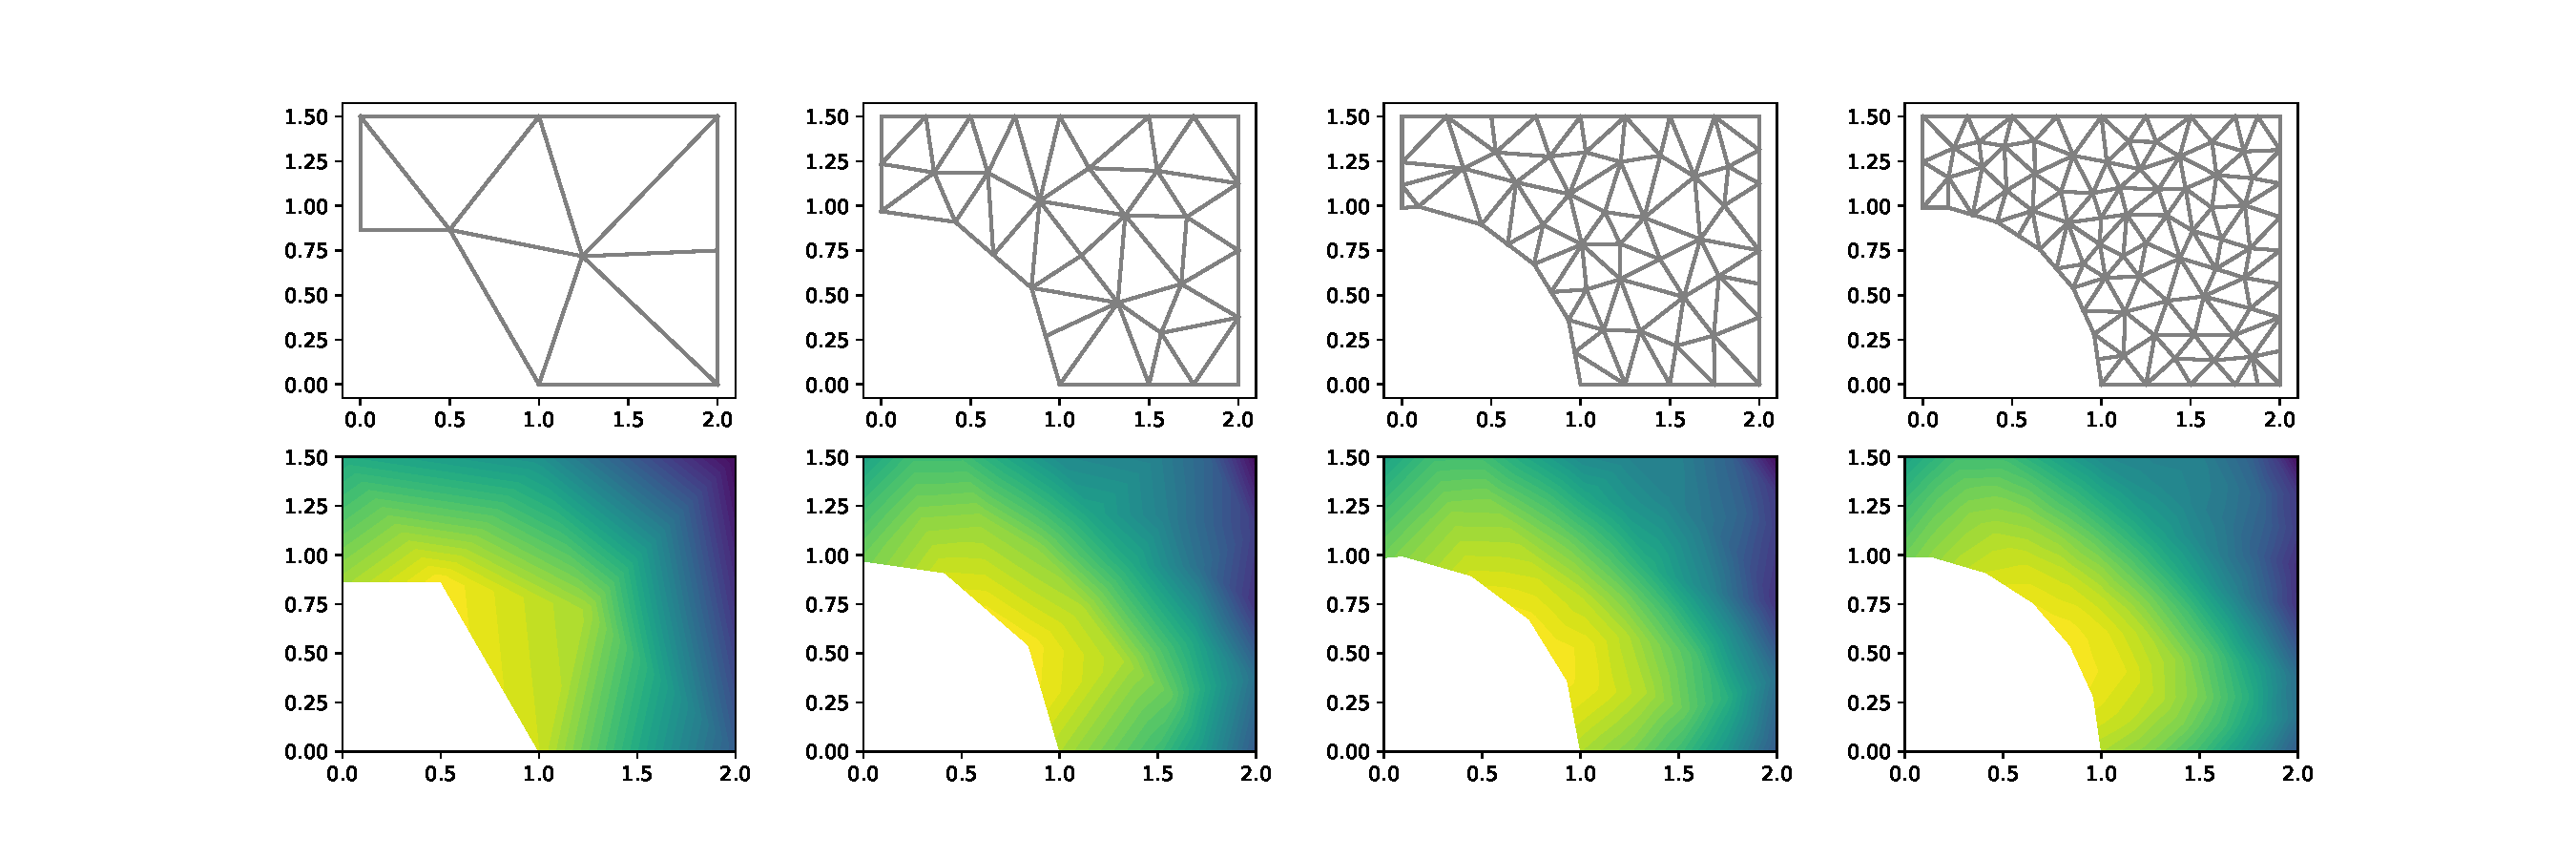
\includegraphics[width=1\textwidth]{intro_figures/mesh_refinement.pdf}
\caption{\small A finite element mesh modeling a rectangular body with an inverse
circular fillet in one corner. Top: the mesh. Bottom: a scalar field $u$ approximated
by a piecewise linear function on this mesh. Left to right: the mesh is refined, leading
to a better approximation of the geometry and the function $u$.}%
\label{Fig:mesh_refinement}%
\end{figure}

-- \emph{Translated laws}. Next, we must translate our mathematical model into a form
which can be applied to the chosen approximate representation.
If the solution is
discretized, the mathematical model must be discretized, i.e. turned into an equation
which the coefficients of the discretized approximate solution should satisfy.
The approximate solution given representation and translated laws should
converge as fast as possible to the true solution as the fidelity parameter is increased,
so that we may obtain an accurate solution without too much computation.
For example, in finite element analysis we first translate the PDE constraint
(such as Poisson's equation, $\delta u(x) = f(x) \forall x \in Omega$) to a
variational form defining what constraints a candidate solution $u \in \mathcal{U}$
should satisfy with respect to test functions $v \in \mathcal{V}$. When $\mathcal{U}$
and $\mathcal{V}$ are sufficiently high-order Sobolev spaces consisting of functions
$\Omega \to \mathbb{R}^d$, we recover the true solution of the PDE $u^*$,
while if we let them be e.g. piecewise polynomials on a
finite element mesh, we retain convergence of the $u \in \mathcal{U}$ which satisfies
the variational form to the true solution as we increase the fineness of the mesh and
the order of the polynomials.
In solving an ODE, we must choose how to go from the law
$\frac{\partial y(t)}{\partial t} = f(t, y(t))$ to a rule in terms of the discrete solution,
$y_{t+1} = y_t + g(t, y_t)$.
Common choices include the forward Euler method,
$y_{t+1} = y_t + \delta_t f(t, y_{t+1})$,
backward Euler, $y_{t+1} = y_t + \delta_t f(t+1, y_{t+1})$ or Runge Kutta methods,
which take multiple trial Euler-like steps and combine the results to achieve
faster convergence with the step size $\delta_t$ \citep{suli2003introduction}.

-- \emph{Numerical solution}. Finally, we must find the solution in the approximating basis
which satisfies the translated laws.
Sometimes, as in the forward Euler method, this step
is direct (just evaluate the right hand side of $y_{t+1} = y_t + g(t, y_t)$ given the current
value of $y_t$).
Sometimes this step requires a numerical subroutine such as an iterative method.
Implicit ODE solvers require a
root finding method; e.g., to find the $y_{t+1}$ which satisfies
$y_{t+1} = y_t + g(t, y_t)$ in the backward Euler method.
In solving PDEs with FEA, we assemble the variational form into a linear or nonlinear system
in terms of the coefficients of the approximate solution in the finite element basis.
If the PDE is linear, we solve the system with a direct or iterative method; if it is
nonlinear, we use an iterative algorithm such as Newton's method or Picard iteration.

For some problems, some of the above steps are trivial, such as
the numerical solution step for the forward Euler method. In other cases,
one or more of the steps may involve numerical subroutines about which whole
textbooks have been written, such as in
FEA, where we must use specialized algorithms to generate a good mesh to represent
the solution, assemble the
variational form into a sparse (non)linear system,
solve the nonlinear system with a
Newton-like method, and solve the linearized system at each step of root finding.

\subsection{Examples of numerical modeling}

\subsubsection{Modeling limits of sequences and series}
One of the oldest examples of numerical modeling is the
\emph{method of exhaustion}, used in ancient Greece and
China to reason about areas and volumes. Archimedes
used this method to estimate the value of $\pi$, by estimating the
area of a unit circle as the limit of a sequence of polygons.

The underlying mathematical law is the relationship $A = \pi r^2$.
However, the area of the circle is not known, so $\pi$ cannot be
determined.
We choose to represent $A$ as the limit of areas $A_n$ of a sequence of
regular polygons each with $n$ sides. Whether the polygon is inscribed
inside the circle ($A^-_n$, where $A^-_n < A$) or outside the circle ($A^+_n$, where $A^+_n > A$), the
difference in areas $|A_n - A|$ can be reduced by increasing $n$.
The sequences $A^+_n$ and $A^-_n$ provide upper and lower bounds on the
value of $A$.
The discretized problem takes the form of a series, with the translated
law $A_n = \hat{\pi}_n r^2$, where $r$ is the radius of the circle
around which or within which the polygon is inscribed.
To solve the problem, one takes the $A_n$ corresponding to
the most many-sided polygon for which one can compute the area
(Archimedes used 96), and uses the
corresponding $\hat{\pi}^+_n$ and $\hat{\pi}^-_n$ as the upper and lower bounds on $\pi$.

\begin{figure}[t]
  \centering
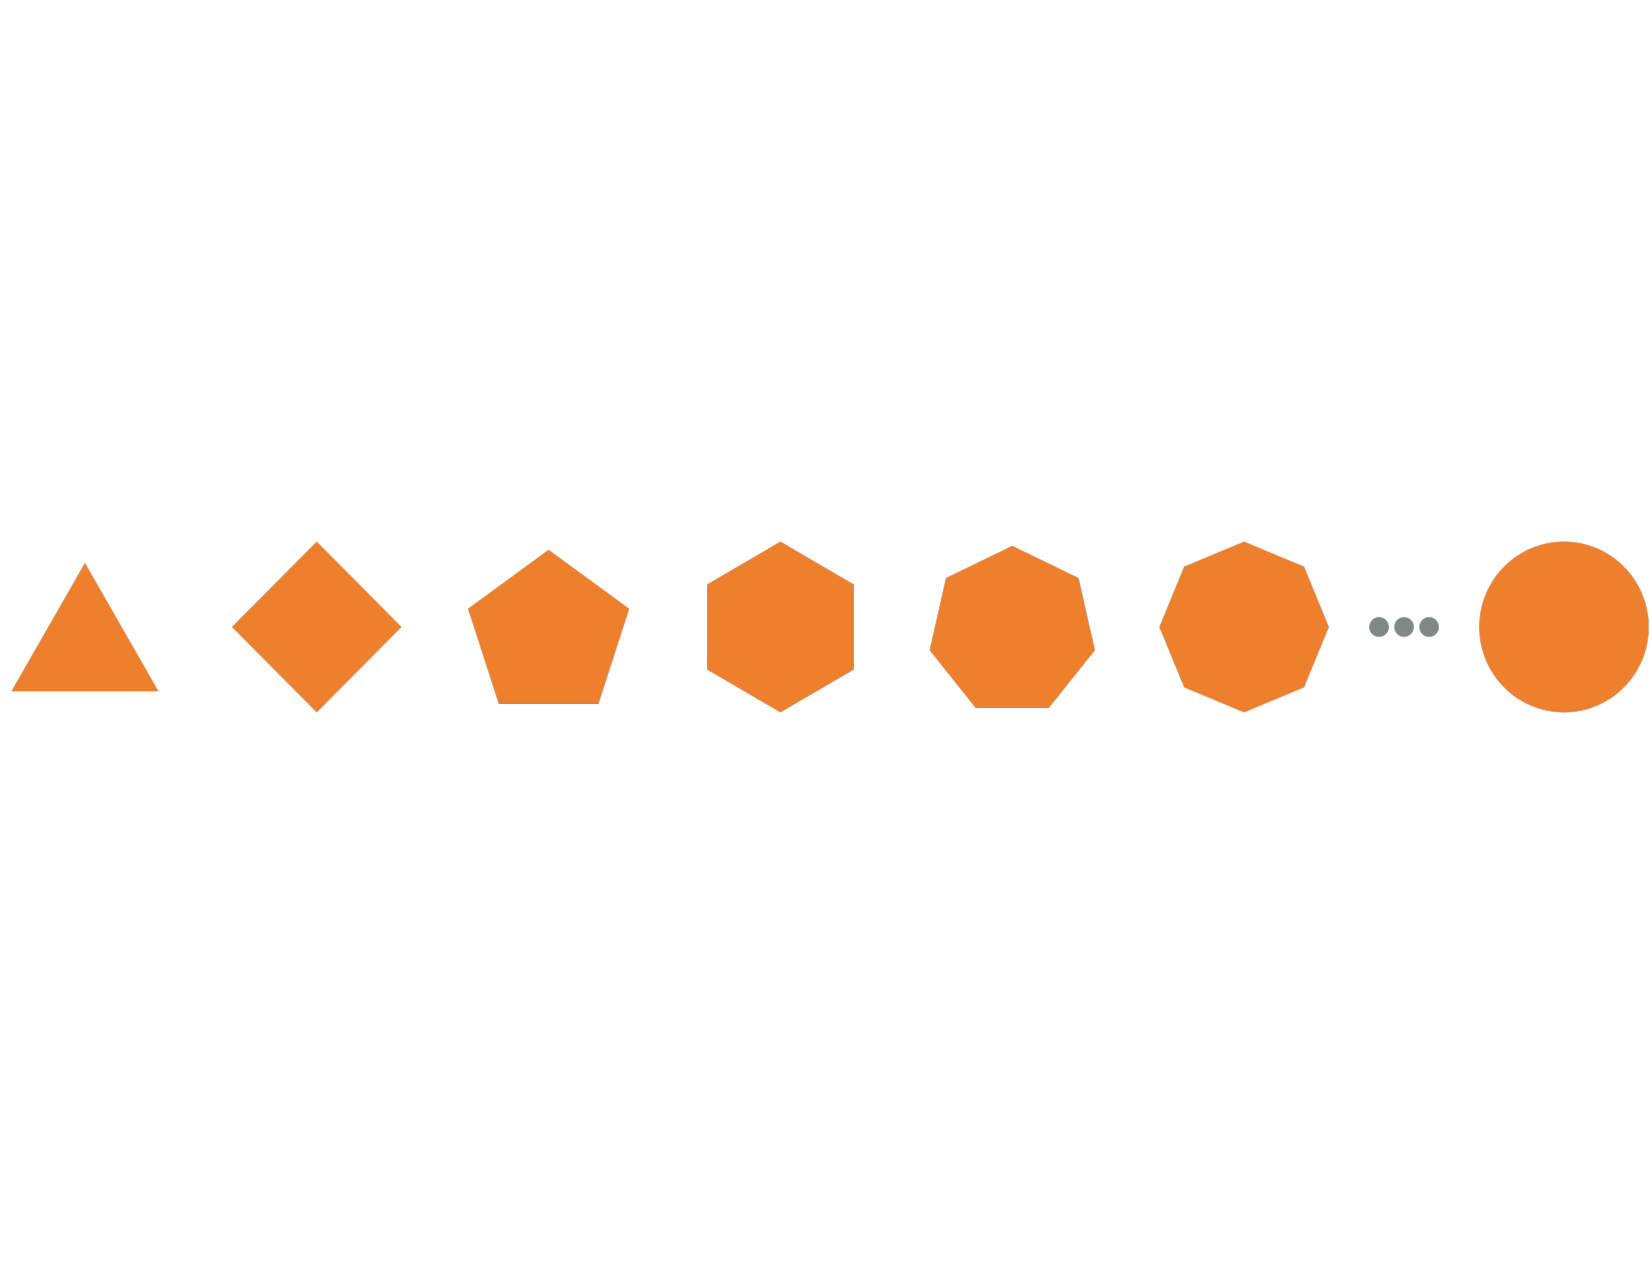
\includegraphics[width=0.9\textwidth]{intro_figures/polygon_cropped.pdf}
\caption{\small Areas of $n$ sided polygons converge to the area of a circle
in the limit $n \to \infty$.}%
\label{Fig:polygon}%
\end{figure}


\subsubsection{Modeling temporal processes with ODEs}
Temporal processes often include a variable of interest $y$ and a
rate of change with respect to time, $\frac{dy}{dt}$, which is a
function of time and the current state: $\frac{dy}{dt} = f(y, t)$.
An example is Newtonian mechanics, such as those governing celestial motion.
Here, $y = [x, v]$, $x, v \in \mathbb{R}^{n \times 3}$ is the
positions and velocities of the $n$ bodies in space ($\mathbb{R}^3$).
We have $\frac{dy}{dt} = [\frac{dx}{dt}, \frac{dv}{dt}] = [v, a]$, where
$a \in \mathbb{R}^{n \times 3}$ is the acceleration of the bodies due to
gravitational force from the other $n$ bodies (which depends on $x$).
While these equations are easily understandable, there is no analytic
solution when $n \geq 3$: even for the three body problem, it is very
hard to reason by hand about all but very special scenarios.

For most $n$-body problems, as for many temporally evolving systems in general, numerical methods are required.
The relation $\frac{dy}{dt} = f(y, t)$ specifies an \emph{ordinary differential equation} or ODE.
To solve them, we usually search for a solution $y(t)$ such that
$\frac{dy}{dt} = f(y, t)$ for all $t$ in the considered time range
$[t_0, t_f]$, given some initial conditions $y_0$.

Usually, we represent a solution in terms of some set of $y_t$, $t = [t_0, t_1, ..., t_N]$: a series
of state values at particular points $t$.
It remains to translate the law $\frac{dy}{dt} = f(y, t)$ to the
discretized system.
The easiest way to do this is to take the forwad Euler method: $y_{t+1} = y_t + f(y_t, t)$, in which case the "numerical solution" step
simply involves evaluating each iterate in turn.
However, much better convergence of the approximate solution to the true solution can often be obtained.
Replacing the \emph{explicit} forwad Euler with an \emph{implicit} method such as the backward Euler, $y_{t+1} = y_t + f(y_{t+1}, t+1)$,
which requires a root-finding algorithm such as Newton's method to numerically solve for each subsequent iterate
$y_{t+1}$, can greatly improve stability and convergence for ODEs
which are "stiff" (i.e., tend to be unstable with explicit solvers,
unless extremely small step sizes are used, even though the solution is
smooth).
Replacing the first-order Euler method (forward, backward, or other)
with a higher order method (such as Runge Kutta or linear multistep methods)
can improve the rate of convergence of the error from $\mathcal{O}(1/N)$,
where $N$ is the number of steps used, to $\mathcal{O}(1/N^p)$, where $p$ is the order of the method.
Runge Kutta methods can be interpreted as (possibly repeatedly) applying \emph{Richardson extrapolation},
a sequence acceleration method discussed later, to Euler's method,
to develop faster-converging approximations.

\subsubsection{Modeling spatial and spatiotemporal systems with PDEs}
Spatial systems and spatiotemporal systems, or other processes which involve
partial derivatives with respect to multiple variables, can often be modeled by
\emph{partial differential equations}, or PDEs.
The solution to a PDE is a field $u$ which maps from a coordinate $x \in \Omega$, where
usually $\Omega \subset \mathbb{R}^{d_1}$, to a value $u(x) \in \mathbb{R}^{d_2}$.
The solution is described by a law $F(u)(x) = 0$, $x \in \Omega$, where
$F$ is a linear or nonlinear operator involving $u$ and its partial derivatives.
For example, in the Poisson equation (a steady-state equation arising often in
electrostatics and fluid
mechanics) we have $d_2 = 1$ (i.e. $u$ is a scalar potential on $\Omega$) and
$F(u) = \delta u - f$, where $f$ is a (possibly spatially varying) source term and
$\delta$ is the Laplace operator; the trace of the Hessian,
$\text{trace}(\frac{\partial^2 u}{\partial x^2})$.
(In physics the Laplace operator is often written as $\nabla^2 u$, however
we avoid this notation as it might confuse a machine learning audience used to
$\nabla^2$ describing a Hessian, not the trace of the Hessian.)
Figure \ref{Fig:poisson} shows an example mesh, source term, and solution for the Poisson
problem on a disc.
In the heat equation we have $F(u) = \frac{\partial u}{\partial t} - \delta u$.
Both of these are \emph{linear} PDEs, i.e. the operator $F$ is linear in
$u$ and/or its partial derivatives, however many systems of interest are
\emph{nonlinear} PDEs.
A simple example is a nonlinear Poisson problem, varieties of which arise in many scenarios
when simplifications used to obtain linearity do not hold. For example,
$F(u) = \text{div}((1 + u^2) \nabla u) - f$, which is equivalent to the standard
Poisson problem when $u \approx 0$.
We usually also have some boundary conditions which constrain the value of $u$
(a "Dirichlet boundary condition") or the derivative of $u$ (a "Neumann boundary condition")
on some or all of the boundary of the domain $\partial \Omega$.

As with ODEs, the equations are simple, but analytic solutions are not available
except for special cases.
This is very often true when $F$ is linear but almost always so when it is nonlinear.
In order to solve PDEs numerically, as we cannot easily reason about arbitrary fields,
we must introduce some approximate family of functions with which to represent $u$.
A common choice is finite elements, employed in \emph{finite element analysis} (FEA).
The domain $\Omega$ is discretized using a mesh and the solution is represented as a
piecewise polynomial with the mesh defining the pieces.

To translate the law $F(u)(x) = 0 \ \in \Omega$ to this discretized space,
FEA first introduces a variational or weak form of the PDE,
$\int_\Omega <F(u)(x), v(x)> dx = 0 \ \ \forall v \in \mathcal{V}$.
Ignoring mathematical subtleties, this weak form is equivalent to the original form
if the family $\mathcal{V}$ is chosen to be the set of all functions mapping from
$\Omega$ to $\mathbb{R}^{d_2}$.
This variational form is amenable to discretization.
Let the family of piecewise polynomial functions representable in the finite element
function space be denoted $\mathcal{V}_{p, n}$, where $n$ is a measure of the number of
mesh elements and $p$ a measure of the polynomial order of the space used, and
consider an approximate solution $u_{p, n}$ in this space.
The translated law is $\int_\Omega <F(u_{p, n})(x), v(x)> dx = 0 \ \
\forall v \in \mathcal{V}_{p, n}$.
To test this constraint it suffices to test the integral is zero for a finite
set of functions which form a basis for $\mathcal{V}_{p, n}$.
We assemble the integral $\int_\Omega <F(u_{p, n})(x), v_i(x)> dx$ for each $v_i$ in
this basis, and rewrite it as a function of $\vec{u}$, the coefficients of the
function $u_{p, n}$ in the piecewise polynomial basis.
The result is a system of equations $\vec{F}(\vec{u}) = 0$,
which $\vec{u}$ must satisfy in order to satisfy
the discretized weak form of the PDE for all $v_i$ forming a basis for
$\mathcal{V}_{p, n}$.
We have translated the continuous law into a numerical system
of equations.
If the PDE is linear, the system will also be linear and we can solve it with an
appropriate method such as QR decomposition or conjugate gradients.
If the PDE is nonlinear, the system of equations will be nonlinear and we will need
to apply an iterative root finder such as Newton's method (which will usually
call a linear solver at each root finding step).
Importantly, as $p$ and $n$ increase and under appropriate conditions, the
solution $u_{p, n}$ which satisfies this system of equations converges to the true
solution $u$ to the PDE.

\begin{figure}[t]
  \centering
\includegraphics[width=10cm]{intro_figures/poisson_equation.pdf}
\caption{\small The Poisson equation on a unit disc. Left: the finite element mesh.
Center: the source term. Right: the approximate finite element solution $u$, found with
FEA. Figure: \citet{xue2020amortized}.}%
\label{Fig:poisson}%
\end{figure}

\subsubsection{Statistical and optimization-based modeling}
Modern machine learning is, naturally, also a form of numerical modeling,
albeit one with a very different flavor to more traditional approaches such as those
for modeling systems with ODEs and PDEs.
We are often interested in a "ground truth" data generating or labeling process or
function, or interested in an optimal control policy or decision rule.
The different flavor of machine learning arises because the description of this function
does not usually come in the form of physical constraints it should obey,
but in the form of some data (e.g., labeled training examples) or interaction
(e.g., state-action sequences of a reinforcement learning agent and the associated
rewards) coupled with a loss function (which might include per-datum losses and
regularization or a prior) we want our function of interest to minimize.
(Bayesian inference instead comes with an observation model, and the goal is to
characterize the posterior distribution over functions or parameters of interest).

Another difference is the function approximation typically employed --
neural networks, kernel methods, and linear models, as opposed to the highly structured
piecewise polynomials and piecewise linear functions often found in physical modeling.
This is in part because the input and sometimes output spaces in machine learning are
usually much higher dimensional than in physical problems where $\mathbb{R}^2$,
$\mathbb{R}^3$, or in general $d < 10$ are the most common.

Nonetheless, there is much similarity. It is hard to reason analytically about the
optimal learned function.
We thus restrict to some family of functions which can be
represented numerically -- e.g. by the weights and biases in a neural network, or
by the data itself (used for interpolation) for Gaussian process regression or a
kernel method.
In the former case, we search for a good function within the function class via
(possibly stochastic) optimization, and query this on new inputs of interest
by passing the data through the neural network.
In the latter case, finding the optimal representation requires no work for an exact GP
(just storage of the data points) but querying the
"learned" function on new data requires solving a large linear system. As with physical models,
we also often wish to place ML-style numerical modeling (whether with NNs, GPs, or
many other methods) within an optimization loop, to find the hyperparameters which give
the best learning performance for a particular task under the metric of interest
(usually, generalization or test error).

\begin{figure}[t]
\centering
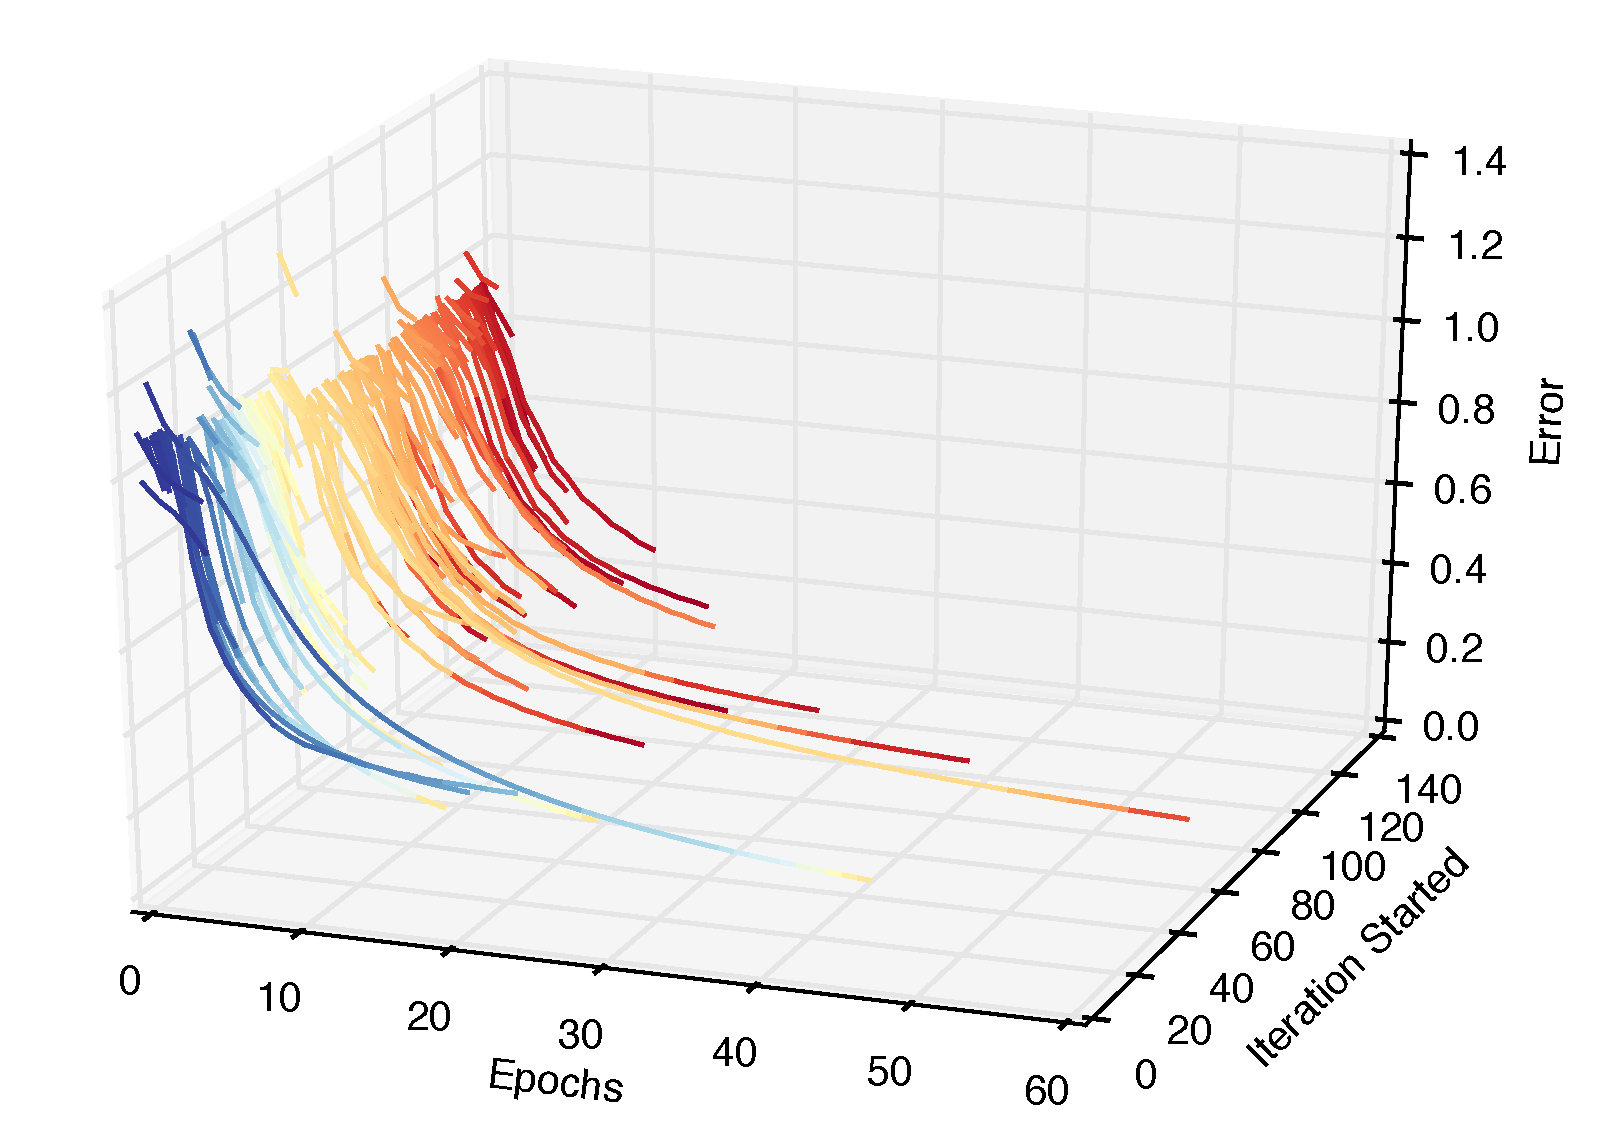
\includegraphics[width=8cm,clip]{intro_figures/inner_loop_opt.pdf}
\caption{\small Learning curves (performance vs epoch) at each iteration of optimizing
the hyperparameters of a neural network. The relative performance with a given
hyperparameter setting at earlier epochs of training
is a useful but imperfect approximation of the performance
at later epochs. Figure: \citet{swersky2014freeze}.}%
\label{Fig:inner_loop_opt}%
\end{figure}

\subsection{The costs of numerical modeling and design}
We have discussed why numerical modeling is
important and the key elements of its application.
Why should we seek to accelerate it with machine learning?

The numerical modeling procedures described above have significant nested
computational and human costs.
These costs are compounded in numerical design and system identification.
Consider, for example, using FEA to perform numerical design when the
design's behavior will be governed by a nonlinear timestepping PDE:

\begin{algorithm}[H]
  \SetAlgoLined
  \caption{Numerical design with FEA}
  \For {each qualitatively different candidate design or component}{
  Define a suitable mathematical model (PDE, BCs, domain) and finite element approximation (mesh, element type, solver)\;
  Define an objective for PDE-constrained optimization (a set of operating conditions and a set of fitness functions to measure the quality of the solution under each operating condition)\;
  \For {each of $G$ gradient steps optimizing the free system parameters}{
  \For {each of $C$ operating conditions}{
  \For {each of $T$ time steps in the simulation}{
  \For {each of $N$ Newton steps solving the nonlinear PDE}{
  Solve a sparse linear system of size $\mathcal{O}(n^d \times n^d)$,
  where we have $n$ elements along each of $d$ spatial dimensions\;
  }
  }
  Use the adjoint method to compute the gradient of the objective\;
  }
  }
  }
\end{algorithm}

The outer \emph{for} loop contains the significant human costs of designing an
appropriate model, discretization, and objective.
Often this process will need to be iterated until results of simulation and optimization
are satisfactory.
Sometimes significant computation will also need to be spent here (e.g. generating a mesh).

The inner \emph{for} loops include significant computational expense from the
many linear system solves required. Unlike in many machine learning workloads,
the cost of computing the gradient of the
objective is not significant next to the cost of running the simulation and computing
the objective. Given a solution and an objective function placed on that solution,
the gradient with respect to the PDE parameters can be taken with the \emph{adjoint method}
\citep{lions1971optimal,mitusch2019dolfin}. Excluding the cost of the adjoint method,
we see
$G \times C \times T \times N$ calls to the linear system solver. Computing the gradient
with the adjoint method has approximately the same cost as solving a linearized form of
the PDE, i.e. a cost of $\mathcal{O}(G \times C \times T)$ solver calls.
The cost of PDE-constrained optimization is dominated by the cost of solving the PDE
at each optimization step.
%\todo{pics}
The cost of each call to the linear solver will depend on the chosen solver and on the
structure of the finite element discretization. For a regular grid on the 2d plane and
using any direct linear solver, there is a lower bound of $\mathcal{O}(n^3)$ computation
for $n$ elements along each spatial dimension (i.e. $n^2$ total elements).
In some cases indirect solvers may do better, and irregular grids may incur extra cost.
However, we can naturally never hope to do better than $\mathcal{O}(m)$ for m total
elements or degrees of freedom (e.g., $m = n^2$ for a regular $n \times n$ grid in $\mathbb{R}^2$)
\citep{hoffman1973complexity}.

How large can we expect this system to be? For small problems, dozens or hundreds of
elements might suffice.
However, modeling complex systems like a rocket engine, a fusion reactor, or a large mechanical structure might use as many as millions of elements.
The engineer must spend significant effort specifying both the design and numerical method,
and may have to wait hours, days, or weeks to see the outcome of a specific simulation,
the results of which might then suggest the need to adjust the design or method.

Of course, engineers make use of approximations to lessen this load.
Such approximations might take the form of splitting a design or system into components
which are simulated separately; introducing approximations into the mathematical
model by e.g. simulating something in 2d instead of 3d, considering steady-state
instead of temporal simulations, or making assumptions about a particular
term in an equation; or simply using a coarser discretization than would be ideal.
These approximations both increase the human effort required and introduce a degree of error.

An important concept is the Pareto frontier of effort (computational or human) vs accuracy.
There will always be a need for new methods or approximations which improve this frontier.
Such new methods not only decrease the human and computer effort required to run existing
workloads, but can increase the accuracy of our numerical modeling (because we no longer have
to cut the corners we once did), and allow us to analyze, identify, and design systems
too large or complex for the previous state of the art.
However, if we introduce a new method, it is important to measure it against the Pareto frontier of an existing method -- not a single point on said frontier.

Consider a situation where we introduce a method for using neural networks to
predict the solution to a PDE from some parameters, and show that this produces
solutions which have only a small amount of error when compared to a given finite
element model, or only 10\% higher error when both methods are compared to some
other known ground truth, while being many
times as fast. This information is not sufficient to say that the new method is useful.
By changing the fidelity of the finite element method (controlled by the density of
the finite element mesh and the polynomial order of the elements) we can also trade off
accuracy for speed, and it might be the case that simply decreasing the density of the mesh
can create the same speed up with the same or less increase in error.
We must measure new methods against a Pareto frontier of the existing methods we compare them to.
Unfortunately, much work in the burgeoning area of machine learning for engineering does
not do this.

We now understand something of the cost of numerical modeling and design, and how
methods to reduce this cost should be evaluated.
In the next section, we discuss how machine learning can be and has been used
to accelerate numerical modeling.

\section{Accelerating numerical modeling with machine learning}

Leveraging approximations to accelerate numerical modeling and design is not a new idea,
and has been an important topic in applied mathematics since at least the early 1900s.
We will first outline a general concept of what we might hope to achieve -- how we
might hope to leverage different sources of information within a problem to better
estimate some quantity without fully resolving it with our numerical model.
Then we will take a brief tour of prior work along these lines, both work focussing on
the general approximation of functions with resolution-speed trade offs, and
work which leverages specific physical or algorithmic structure of simulations.
It is not possible for this section to be exhaustive, and there will be much important
work that we miss for the sake of brevity.

\subsection{What can we hope to achieve?}

Generally speaking, we can consider some baseline numerical model $f$ which acts on some
representation of the scenario or design $\phi$ and returns a quantity of interest $y = f(\phi)$.
We wish to approximate $y$ without running $f$ (to avoid the expense involved),
instead taking $y \approx \hat{f}(\phi)$, where $\hat{f}$ is our approximate model.

\subsubsection{Sources of information}
If we are not to call $f$, then $\hat{f}$ must use some information about $f$
available from one or more other sources in order to provide better-than-arbitrary
estimates of $y$. What such sources of information are available?
Many methods will use more than one of the following, and we discuss examples of each
in both the overview of existing approaches and in the research contributions of
the thesis.


\begin{itemize}
  \item \emph{Results of cheaper or lower-fidelity simulations $y_i = f_i(\phi)$.}
  In numerical modeling we often have access to some sequence of approximations $f_i$,
  where as $i \to \infty$, $y_i = f_i(\phi)$ converges to the true quantity we are
  interested in, but so does the difficulty or cost of evaluating $f_i$.
  If we know something about the convergence properties of the sequence of models $f_i$,
  this knowledge might allow us to use evaluations of some of the
  models $f_{1:i-1}$ to approximate the result of $f_i$ as
  $\hat{y}_i = \hat{f}_i(y_1, y_2, ... y_{i-1})$ without evaluating it.
  A quintessential example of this is \emph{sequence acceleration}
  \citep{osada1991acceleration}, discussed in the
  next section. \\
  \item \emph{Results of simulation of similar problems, $y' = f(\phi')$.}
  Given a training set consisting of parameterizations of particular problems $\phi_i$
  and the solutions to those problems $y_i$, we may try to learn an approximation
  $\hat{f}$ to the function/model $f$ which is cheaper to evaluate than $f$ itself.
  A quintessential example of this is surrogate modeling via simply regressing from the
  training $\phi_i$ to the target solutions $y_i$.\\
  \item \emph{Known computational or physical structure associated with the
  model $f$.} This is a broad category.
  In many cases, leveraging known computational
  structure in the numerical model $f$ or known physical or mathematical properties of
  the system $f$ approximates will improve methods which rely on generalization from
  lower-fidelity iterates $f_{<i}$ or from similar problems $y' = f(\phi')$.
  However, leveraging this structure can also be used to design new numerical models
  $y \approx \hat{f}(\phi)$ which can be used as simulators without requiring information from
  $f$ for training or evaluation.
\end{itemize}

\subsection{Extrapolation and sequence acceleration}
One of the earliest examples of work with a similar flavor to that in this thesis
is the subfield of applied mathematics concerned with \emph{sequence acceleration} or
\emph{series acceleration}.
See \citet{osada1991acceleration} for an excellent overview.
Much of the key work in sequence acceleration was done in the early 20th century, however some early transformations were known to Stirling, Euler,
Maclaurin, and Seki Kowa.

Given a sequence $s_n$ which converges to a limit, $\lim_{n \to \infty} s_n = s^*$,
sequence acceleration is concerned with constructing a transformed sequence $s'_n$
which converges to the same limit but with a faster rate of convergence.
This can be restated as designing a transformation operator $\mathcal{T}$, where
$s'_n = \mathcal{T}(s_n, s_{n-1}, ..., s_1)$.
Formally, $\mathcal{T}$ accelerates the sequence if
$\lim_{n \to \infty} \frac{s'_n - s^*}{s_n - s^*} = 0$.
However, we are often interested not in just whether $\mathcal{T}$ accelerates the
sequence but in how fast the new convergence of $s'_n$ to $s^*$ is: e.g.
if the sequence is polynomially converging, $|s'_n - s^*| = \mathcal{O}(\nicefrac{1}{n^p})$,
we would like $p > 0$ to be as high as possible,
whereas it would be even better if it were geometrically converging,
$|s'_n - s^*| = \mathcal{O}(1-p)^n$, where we would like
$ 0 < p < 1$ to be as large as possible.
These are often called logarithmic and linear convergence in cases
where the studied quantity is not the big-O behavior of $|s_n - s^*|$ but the limiting
ratio of subsequent errors,
$\lim_{n \to \infty} \frac{|s_{n+1} - s^*|}{|s_n - s^*|}$.

These methods can be used to accelerate numerical modeling when we have some
parameter which trades off computation or effort for fidelity: for example, the
resolution of a finite element mesh, or the number of steps or inverse step-size used to solve an ODE,
or the number of iterations in a Newton method or in an optimization procedure
used to train a neural network.
In such cases, we are often interested in
the limit of some quantity as we allow an unbounded amount of computation.
However, we only have a finite computational budget.
Given this finite budget, we might hope that by evaluating the quantity of interest
at several different fidelities ($s_1 ... s_n$), we might be able to extrapolate
($s'_n$) to get a better estimate of the limit $s^*$ than using $s_n$ alone.

It is not possible to find an operator $\mathcal{T}$ which accelerates all sequences.
Some assumptions must be made about the original sequence, e.g. its original rate of
convergence, and it is also useful to know if the sequence is asymptotically alternating
or monotonic.

Each sequence acceleration method has a class of sequences which it will accelerate.
Two of the most famous methods are \emph{Richardson extrapolation}, for polynomially
convergent sequences, and \emph{Aitken's delta-squared method}, for geometrically
convergent sequences.

Richardson extrapolation is designed for sequences which have an asymptotic
expansion $s_n = s^* + C \nicefrac{1}{n^p} + \mathcal{O}(\nicefrac{1}{n^{p+1}})$. (Often, $n$ is the inverse of the
step-size of an ODE integrator).
We choose some factor $\tau > 1$ and construct the extrapolation
\[
R(n, \tau) = \frac{\tau^p s_n - s_{n/\tau}}{\tau^p - 1}
\]
We then have:
\begin{align*}
R(n, \tau)(\tau^n - 1) &= \tau^p(s^* + C \nicefrac{1}{n^p} + \mathcal{O}(\nicefrac{1}{n^{p+1}})) - (s^* + C \nicefrac{1}{(n/\tau)^p} + \mathcal{O}(\nicefrac{1}{(n/\tau)^{p+1}}))\\
\implies R(n, \tau) &= s^* + \mathcal{O}(\nicefrac{1}{n}^{p+1})
\end{align*}
Thus, Richardson extrapolation eliminates the $C \nicefrac{1}{n^p}$ term in
the asymptotic expansion of $s_n$, giving a higher order / faster converging error
$\mathcal{O}(\nicefrac{1}{n^{p+1}}$.

Aitken's delta-squared process is the transformation:
\[
s'_n = \frac{s_n s_{n-2} - s_{n+1}}{s_n + s_{n-2} - 2*s_{n-1}},
\]
or equivalently,
\[
s'_n = s_n - \frac{(s_n - s_{n-1})^2}{s_n - 2 s_{n-1} + s_{n-2}}
\]

Aitken's delta-squared process accelerates any geometrically (or linearly)
convergent sequence.
As opposed to Richardson extrapolation, which eliminates the slowest polynomial error term, Aitken's delta-squared process can be thought of as eliminating the slowest geometric error term.
If the series has an asymptotic expansion $s_n = s^* + a^n$ with $0 < a < 1$, then the transformation is exact ($s'_n = s^*$) for all $n$. If the series has an asymptotic expansion $s_n = s^* + a^n + \mathcal{O}(b^n)$   where $0 < b < a < 1$, then the transformed series has the asymptotic
expansion $s'_n = s^* + \mathcal{O}(b^n)$, i.e. eliminating the slower
$a^n$ term.

Sequence acceleration methods are not today very commonly used by practitioners.
However, as well as being of historical and intellectual interest,
they underpin a number of fast-converging
numerical methods for various applications,
which can be derived by application of one of these
sequence acceleration methods to a "base" numerical method.
For example, higher-order Runge-Kutta methods for ODE integration can be derived from
first-order Euler methods by repeatedly applying Richardson extrapolation
$p-1$ times to achieve a method with convergence of order $p$.
(Runge-Kutta methods slightly predate Richardson's introduction of his general
extrapolation scheme, but their motivation, method and analysis is an exact application
of the extrapolation).
Richardson extrapolation is also used to derive Romberg's method for integration by repeated application to the trapezium rule.
Aitken's delta-squared process can be applied to a fixed point
iteration to derive Steffenson's method, which has quadratic convergence (a la Newton's method) while not requiring derivatives.
Historically, sequence acceleration methods have been applied to one-dimensional sequences,
and they can sometimes be lacking when applied naively to higher-dimensional problems (e.g., Steffenson's method runs into a "curse of dimensionality" with high-dimensional root-finding problems).
Much of the work on sequence acceleration in recent decades has
been on extending or developing methods for vector sequences \citep{osada1991acceleration}.


\subsection{Surrogate modeling}
A natural approach to accelerating numerical modeling is to regress from a parameter
of the design or factor of variation of the numerical model
on to the solution (or a quantity of interest associated with the solution).
This regression model provides a \emph{surrogate model} for the base simulator.
If the surrogate model is accurate, it can be queried in place of the simulator to
do analysis, optimization or system ID -- i.e., to answer questions about the
system's behavior in particular scenarios, the optimality of designs, or the
likelihood of system parameters given observations.

Any and every regression method can and has been used for such tasks --
linear regression, polynomial regression, kernel methods, neural networks, and more.
For overviews of the broad volume of work in this area, see \citet{simpson2001metamodels,martin2005use,queipo2005surrogate,
koziel2013surrogate,willard2020integrating}.
A distinction beyond the regressor is \emph{what is predicted}.
One route is to directly predict the solution $y$ to a numerical model $f$ with parameters
$\phi$, $y = f(\phi)$, using the learned regressor: $y \approx \hat{f}(\phi)$.
This lets one use the surrogate to answer whatever questions one wishes about the
solution $y$.
However, $y$ might be indexed by a high-dimensional vector of coefficients, and
the learning task of predicting $y$ from $\phi$ might be very hard.
Worse, the way in which $y$ is represented (e.g., the size and meaning of the vector
of coefficients) might change depending on $\phi$: e.g. if changing $\phi$ means
a problem domain is larger or smaller, or has different geometry.
This will break many regression models.
As such, it is sometimes more useful to choose an alternate quantity to predict.
If one is interested in the performance of a design, measured by an objective function,
then one can predict that scalar objective value directly from $\phi$ without
modeling the solution.
This could be an easier learning problem if, for example, there are ranges of $\phi$
which cause large, unstable variations of the solution but which all have a poor
objective value.

Another choice is possible when simulation can be framed as a bi-level
problem.
In this scenario, the solution to one or more "inner" problems $z = g(\gamma)$
is used when solving the "outer" problem $y = f(\phi)$, and where $g$ is the solution
procedure for the inner problem; $\gamma$ are the parameters, and $z$ is the output
of the inner problem.
The inner problem(s) might have more regularity than the outer problem -- i.e.,
the mapping $z = g(\gamma)$ may be easier to learn, or the outer problem solution
representation $y$ may change significantly with $\phi$ while the inner solution
representation $z$ does not -- often this occurs when $g$ may be called multiple times,
varying with $\phi$, to compute $z_{1..l}$ which are used in computing $y$.
If a surrogate model for $g$ would significantly reduce the cost of one full solution,
training a surrogate $z \approx \hat{g}(\gamma)$ and using this as a component in the
numerical model for $y$ may be an effective strategy.
For example, \citet{tompson2017accelerating} accelerate solving linear systems which
are the computational bottleneck for Eulerian simulation of the Navier-Stokes
equations, while in \citet{beatson2020learning} we accelerate computing strain energies
and strain energy gradients which must be computed at each Newton iteration of solving
a continuum mechanics PDE.

One other factor of interest for surrogate models is the training method.
Naively applying regression requires one to solve many "full" simulations
to generate training data, and is thus only useful if one would otherwise need
to query the simulator many more times than the number of training points required
(which might be thousands).
Instead training a model to predict the solution of some sub-problem can allow
training data to be generated much more cheaply
\citep{tompson2017accelerating,beatson2020learning}.
Another avenue is to exploit the particular structure of the numerical model to avoid
the need to call the original simulator entirely, e.g. by learning a model
$y \approx \hat{f}(\phi)$ by minimizing some physically-motivated loss
$\mathcal{L}(y, \phi)$ which is also minimized by the solution to the original
numerical model $f$ \citep{xue2020amortized}.

\subsection{Model order reduction}
Rather than predicting the outcome of a simulation or of one of the subroutines in the
simulation, \emph{model order reduction} methods learn a solution basis which allows for
more efficient simulation.
Most of them rely on a projection operator to project the solution to a
lower-dimensional latent space (or return it from this to the full solution space).
The laws governing the numerical model must then be approximated by some laws in the
latent space which give rise to a similar result.

The most well known method is the \emph{proper orthogonal decomposition} (POD) \citep{chatterjee2000introduction}, used to
reduce the complexity of finite element simulations.
POD involves performing principal component analysis on some set of observations,
called snapshots, of $y$, where the solution $y$ to the numerical model is a field of
interest such as the velocity, density and pressure fields in a Navier-Stokes simulation.
We represent $y_i(x) = \sum_{k=1}^K \alpha_{i,k} \eta_k(x)$, where $\eta_k$ are the
principal components, $y_i$ are the solutions at different times or for different
systems or designs, $\alpha_{i, k}$ are the weights, and $x$ is a coordinate in the
domain $\Omega$.
As with PCA in machine learning, the POD is often used for understanding and visualizing
data, which in the POD's case arises from real-world experiments or from simulation.
However, the POD is also used as a tool to accelerate simulation, by projection of the
linear system governing the finite element model, $A\vec{y} = b$, into a lower
dimensional space, $A' \vec{\alpha} = b'$.

Another dimension reduction method related to the work in this thesis is static
condensation, or Guyan reduction \citep{guyan1965reduction}.
In finite element analysis it is often the case that only some degrees of freedom
(often those on the boundary) may be "loaded" (have values constrained via
Dirichlet boundary conditions or external forces imposed via Neumann boundary conditions)
while the others are "unloaded" and will always be governed by the same physical laws,
regardless of the loading scenario.
Static condensation provides a way to develop an \emph{exact}
reduced-order model when the only factor of variation is the load or boundary
conditions imposed and when the underlying PDE is linear.
Using finite element analysis, we write the coefficients of the solution in the finite
element basis in terms of a linear system $A\vec{y} = b$.
This can be partitioned in terms of the free and loaded degrees of freedom as:
\[
\begin{bmatrix}
A_{l,l} & A_{l,f} \\
A_{f,l} & A_{f,f}
\end{bmatrix}
\begin{Bmatrix}
  \vec{y}_l \\
  \vec{y}_f
\end{Bmatrix} =
\begin{Bmatrix}
  b \\
  0
\end{Bmatrix}
\]
This linear system is rearranged to eliminate $\vec{y}_f$, and be written in terms of
$\vec{y}_l$ alone.
This might be useful when, for example, we are modeling a system formed of multiple
components and for many of the components we are not interested in the internal degrees
of freedom -- only in how those components interact with others via the boundary.

The above methods are linear, and typically are restricted to linear or
approximately linear PDEs.
Developing model order reduction methods for nonlinear PDEs is an exciting area for
machine learning (which has seen a lot of recent work on learning nonlinear schemes
for compressing data to latent representations with neural networks).
We present some work along this line in the thesis.
Other interesting recent work in the same theme includes
\citet{bar2019learning}, \citet{maulik2021reduced}, and many more.

\subsection{Randomized methods}
A concept and approach somewhat orthogonal to the aforementinoed methods
is to reduce computation via randomization.
Often, this involves using randomization as an important tool within e.g.
projection-based model order reduction methods.
Random snapshot selection can, given a suitable distribution over snapshots, quickly
converge to a basis which can represent the solution with smaller error.
In other cases, this involves using randomization to speed up a core subroutine of
the numerical solution procedure.
For example, randomized algorithms can be used to provide fast approixmations to the
matrix SVD or to the solution of linear systems
\citep{drineas2006fast,drineas2016randnla}, by projecting the system with a
random matrix (often of i.i.d. Gaussian vectors) to a lower-dimensional subspace.

Possibly the most well-known use of randomness to accelerate computation is the use
of stochastic gradient descent in machine learning
\citep{robbins1951stochastic,bottou2010large}.
Given a large dataset, it is computationally prohibitive to estimate the gradient of a
model's loss averaged over all examples in the dataset.
However, if we randomly choose a batch of examples on which to compute and average
the loss, the gradient of this loss is a random but unbiased estimator of the full
gradient, with variance depending on the size of the batch.
Using this gradient estimator for first-order optimization can lead to much faster
optimization (in terms of reduction of the loss as a function of computational effort)
than the full-batch gradient, especially as the size of a dataset increases, and
particularly as most datasets have some covariance between per-example gradients
(i.e. many examples in the dataset may have similar loss and gradient functions).
In \citep{beatson2019efficient}, included in this thesis, we show how to
build a cheap stochastic gradient estimator for objectives involving
discretization-based numerical models.

\section{Research contributions in this thesis}

In this thesis we present some recently developed methods for accelerating
numerical modeling, simulation, and design.
This work has been been the fruit of collaboration with a number of wonderful
colleagues, without whom it the work would not have been possible, and without whom
I would have learned far less and had infinitely less fun.

In \textbf{Chapter 2} we present \emph{composable energy surrogates} \citep{beatson2020learning};
a method which leverages
modular structure to learn component-level surrogates for modular PDEs; specifically
those governing mechanical meta-material deformation.
These mix attributes of surrogate modeling and model order reduction, and allow
learning of fast approximate solvers while only using supervision from data collected
by solving cheap PDEs governing component subregions, rather than requiring data
collected by solving the PDEs governing the full system we wish to solve in deployment.
This work was presented at NeurIPS 2020 and was carried out in collaboration with
Jordan T. Ash, Geoffrey Roeder, Tianju Xue, and Ryan P. Adams.

In \textbf{Chapter 3} we present \emph{randomized telescoping gradient estimators} \citep{beatson2019efficient}, which are
randomized gradient estimators for objectives which are the limit of a sequence of
approximations (as when performing optimization or design with numerical models).
By randomizing the fidelity of the approximation, we obtain unbiased gradient estimators
which trade computation for variance.
We provide recipes for choosing within the family of such estimators and demonstrate
their effectiveness in system identification and machine learning hyperparameter
optimization.
This work was presented at ICML 2019
and was carried out in collaboration with Ryan P. Adams.

In \textbf{Chapter 3},
we present \emph{meta-learned implicit PDE solvers} (Meta-PDE), which are neural networks
representing PDE solution fields, which have initializations meta-learned across a
family or distribution of PDEs such that they converge quickly to represent the solution
of a given PDE in a few gradient steps of minimizing that PDE's variational energy.
This provides a surrogate modeling method which is agnostic to geometry and is mesh-free:
while many other surrogate modeling techniques require a geometry and mesh to be fixed
across the family of problems they amortize, this method only requires the user to
supply a sampler for the variational energy of (or a sampler for the geometric domain of)
each problem within the family to be amortized -- usually a much easier task.
This work is in preparation for publication, and has been
carried out in collaboration with Sunny T Qin, Nick McGreivy, and Ryan P. Adams.

Beyond the work presented in the thesis, these themes and ideas have been
both cultivated by and continued in papers led by
other phenomenal researchers with whom I've had the pleasure of collaborating.
"SUMO: Unbiased Estimation of Log Marginal Probability for Latent
Variable Models" \citep{luo2019sumo},
led by Yucen Luo and Ricky Chen, demonstrates
an important application of randomized telescope-like estimators to
variational inference.
"Randomized Automatic Differentiation" \citep{oktay2021randomized},
led by Deniz Oktay, uses similar philosophy to
randomized telescopes to develop a stochastic gradient method for a
regime beyond the usual one of a separable dataset,
but in this case for the general setting of linearizable computational graphs.
In \citep{ravi2018amortized},
led by Sachin Ravi, Sachin and I
realized the potential of meta-learning as a tool for amortizing
optimization and computation (rather than "just" being a tool for
few-shot generalization), which is a crucial principle for Meta-PDE;
our time thinking hard about bi-level optimization also
helped ferment the other two chapters.
Finally,
"Amortized Finite Element Analysis for Fast PDE-Constrained Optimization"
\citep{xue2020amortized},
led by Tianju Xue, laid the foundation for the Meta-PDE
project by establishing the principle of using a neural network to
minimize a variational energy rather than a supervised loss,
avoiding expensive training data generation for surrogate modeling.


\chapter{Learning composable energy surrogates for PDE order reduction}

\section{Abstract}
Meta-materials are an important emerging class of engineered materials in which complex macroscopic behaviour--whether electromagnetic, thermal, or mechanical--arises from modular substructure.
Simulation and optimization of these materials are computationally challenging, as rich substructures necessitate high-fidelity finite element meshes to solve the governing PDEs.
To address this, we leverage \emph{parametric} modular structure to learn component-level surrogates, enabling cheaper high-fidelity simulation.
We use a neural network to model the stored potential energy in a component given boundary conditions. This yields a structured prediction task: macroscopic behavior is determined by the minimizer of the system's total potential energy, which can be approximated by composing these surrogate models. Composable energy surrogates thus permit simulation in the reduced basis of component boundaries. Costly ground-truth simulation of the full structure is avoided, as
training data are generated by performing finite element analysis of individual components. Using dataset aggregation to choose training data allows us to learn energy surrogates which produce accurate macroscopic behavior when composed, accelerating simulation of parametric meta-materials.

\vspace{-0.2cm}\section{Introduction}\vspace{-0.2cm}
Many physical, biological, and mathematical systems can be modeled by partial differential equations (PDEs).
Analytic solutions are rarely available for PDEs of practical importance; thus, computational methods to approximate PDE solutions are critical for many problems in science and engineering.
Finite element analysis (FEA) is one of the most widely used techniques for solving PDEs on spatial domains; the continuous problem is discretized and replaced by basis functions on a mesh.

The accuracy of FEA and related methods requires a sufficiently fine discrete approximation, i.e., finite element mesh.
Complicated domains can require fine meshes that make it prohibitively expensive to solve the PDE.
This problem is compounded for parameter identification or design optimization,
where the PDE must be repeatedly solved in the inner loop of a bi-level optimization problem.

An important domain where this challenge is particularly relevant is in modeling mechanical meta-materials.
Meta-materials are solids in which microstructure leads to rich spaces of macroscopic behavior, which can achieve electromagnetic and/or mechanical properties that are impossible with homogenous materials and traditional design approaches \citep{poddubny2013hyperbolic,cai2010optical,bertoldi2017flexible}.
We focus on the \emph{cellular} mechanical meta-materials proposed by \citet{overvelde2014relating}, which promise new high-performance materials for soft robotics and other domains (see Sec 3).
Simulation of these meta-materials is challenging due to the need to accurately capture microstructure and small-scale nonlinear elastic behavior.
Finite element methods have limited ability to scale to these problems, and automated meta-material design demands accurate, efficient approximate solutions to the associated PDE.

We develop a framework which exploits spatially local structure in large-scale optimization problems---here the minimization of energy as a function of meta-material displacements.
Only a small subset of material displacements are of interest, so we ``collapse out'' the remainder using a learned surrogate.
Given a component with substructure defined by local parameters, the surrogate produces an accurate proxy energy in terms of the displacement of the component boundary.
A single surrogate can be trained then used to predict energy in a larger solid by summing energies of sub-components.
This allows solving the PDE in a reduced basis of component boundaries by minimizing this sum.

Other methods exist for reducing the solution cost of large PDEs. One such is the boundary element method \citep{aliabadi2002boundary}, which as with our method "collapses out" the internal degrees of freedom in a PDE leaving a problem in terms of the solution on the boundary. Unlike our method, this is performed analytically and is typically only valid for linear PDEs. Our method might be seen as a \emph{learned} boundary element method for a particular parametric class of nonlinear PDEs. Another related line of work is homogenization. Whether micro-scale effects are modeled with fine-resolution FEM \citep{schroder2014numerical} or a neural network \citep{xue2020data}, homogenized models require a PDE formed of homogenous representative volume elements (RVEs), and are accurate only as the ratio between the size of the RVE and the size of the macro-scale problem tends to zero.

Some approaches amortize PDE solving more directly, using neural networks to map from PDE parameters to solutions \citep{zhu2019physics,nie2020stress} or constructing reduced bases via solving eigenvalue problems or interpolating between snapshots \citep{berkooz1993proper, chatterjee2000introduction}.
These approaches typically require solving full systems to produce training data.
Our framework uses the modular decomposition of energy to train surrogate models on data generated by querying the finite element "expert" on the energy in small components, avoiding performing FEA on large systems which are expensive to solve.

\section{Learning to optimize in collapsed bases}
\label{sec:collapsed}
Solving PDEs like those that govern meta-material behavior involves finding a solution~$u$ which minimizes an energy~$E(u)$ subject to constraints.
For mechanical meta-materials, $E(u)$ is the stored elastic potential energy in the material.
We propose a framework for amortizing high-dimensional optimization problems where the objective has special conditional independence structure, such as that found in solving these PDEs. Consider the general problem of solving
\small\begin{equation}\label{eq:minimization}
u^* = \argmin E(u)\,.
\end{equation}\normalsize
~$u$ may be a vector in~$\mathbb{R}^d$ or may belong to a richer space of functions.
Often we are interested in a subset of the vector~$u^*$, or the values the function~$u^*$ takes on a small subdomain.
To reflect this, view the solution space as the Cartesian product of a space of primary interest and a ``nuisance'' space.
Denote the solutions as concatenations~${u=[x,y]}$ where~$y$ is the object of interest, and~$x$ is the object whose value is not of interest to an application.
~$x$ is roughly similar to auxiliary variables that appear in probabilistic models, but are marginalized away or discarded from the simulation.
We use this decomposition to frame Eq.~\ref{eq:minimization} as a bi-level optimization problem:
\begin{equation}\label{eq:bilevel}\small
y^* = \argmin_y \min_x E(x, y)\,.
\end{equation}
Consider the \emph{collapsed objective},~${\tilde{E}(y) = \min_x E(x, y)}$.
If~$\tilde{E}(y)$ can be queried without representing~$x$, we may perform \emph{collapsed optimization} in the reduced basis of~$y$,
avoiding optimization in the larger basis of~$u$ (Eq. \ref{eq:minimization}), or performing bi-level optimization (Eq. \ref{eq:bilevel}). However, ~$\tilde{E}$ is not usually available in closed form.
We consider approximating~$\tilde{E}(y)$ via supervised learning.
In general, this would require solving~${\tilde{E} = \min_x E(x, y)}$ for each example~$y$ we wish to include in our training set.
This is the procedure used by many surrogate-based optimization techniques \citep{queipo2005surrogate,forrester2009recent,shahriari2015taking}.
The high cost of gathering each training example makes this prohibitive when~$x$ is high dimensional (and minimization is difficult) or when~$y$ is high dimensional (and supervised learning requires many examples). Compositional structure in~$E$ may assist us with approximating~$\tilde{E}$.
Many objectives may be represented as a sum:
\begin{equation}\label{eq:sum}\small
    E(x, y) = \sum_i E_i(x_i, y)\,.
\end{equation}
Given this decomposition,~$x_i$ and~$x_j$ are conditionally independent given~$y$; i.e., if we constrain~$x_i$ and~$y$ to take some values and perform minimization, the  resulting $x_j$ or $E_j(x_j, y)$ do not vary with the value chosen for $x_i$.
This follows from the partial derivative structure~${\frac{\partial{E_i}}{\partial x_j} = 0}$ for~${i\neq j}$.

We propose to \emph{learn} a collapsed objective $\tilde{E}$, which exploits conditional independence structure by representing~${\tilde{E}(y) = \sum_i \tilde{E}_i(y)}$.
This representation as a sum allows us to use~${\min_{x_i} E_i(x_i, y)}$ as targets for supervision, which may be found more cheaply than performing a full minimization.
The learned approximations to~$\tilde{E}_i$ may be composed to form an energy function with larger domain.

The language we use to describe this decomposition is chosen to reflect the conceptual similarity of our framework to \emph{collapsed variational inference} \citep{teh2007collapsed} and \emph{collapsed Gibbs sampling} \citep{geman1984stochastic, liu1994collapsed}, in which conditional independence allows optimization or sampling to proceed in a collapsed space where nuisance random variables are marginalized out of the relevant densities.
We exploit similar structure to these techniques, albeit in a deterministic setting.
Other approaches to accelerating Eq.~\ref{eq:bilevel} which do not exploit (\ref{eq:sum}) or directly model~$\tilde{E}(y)$ include amortizing the inner optimization by predicting~${x^*(y) = \argmin_x E(x, y)}$ \citep{kingma2013auto,brock2017smash}, or truncation of the inner loop, either deterministic \citep{wu2018understanding,shaban2018truncated} or randomized to reduce bias \citep{tallec2017unbiasing,beatson2019efficient}.

The optimization procedure we accelerate is the simulation of mechanical materials, where the objective corresponds to a physically meaningful energy, and the conditional independence structure arises from spatial decomposition of the domain and spatial locality of the energy density.
We believe this spatial decomposition of domain and energy could be generalized to learn collapsed energies for solving many other PDEs in reduced bases.
This collapsed-basis approach may also be applicable to other bi-level optimization problems where the objective decomposes as a sum of local terms.
\vspace{-0.1cm}

\section{Mechanical meta-materials}
\label{sec:metamaterials}
Meta-materials are engineered materials with microstructure which results in macroscopic behavior not found in nature.
The most popularly known are electromagnetic meta-materials such as negative refraction index solids and ``invisibility cloaks'' which conceal an object through engineered distortion of electromagnetic fields \citep{poddubny2013hyperbolic,cai2010optical}.
However, they also hold great promise in other domains: \emph{mechanical} meta-materials use substructure to achieve unusual macroscopic behavior such as negative Poisson's ratio and nonlinear elastic responses; pores and lattices undergo reversible collapse under large deformation, enabling the engineering of complex physical affordances in soft robotics \citep{bertoldi2017flexible}.
\begin{wrapfigure}[12]{r}{0.4\textwidth}
\vspace{-0.2cm}
\centering
\begin{tabular}{c|c|c}
  		 {{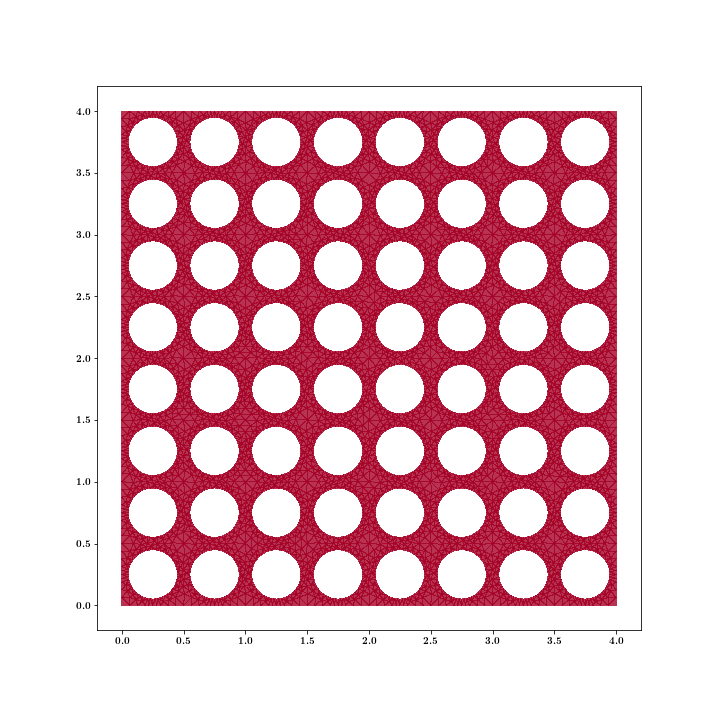
\includegraphics[height=1.1cm, trim={3.5cm 3.5cm 3.5cm 3.5cm}, clip]{lces/figures/rest_pore_0} }}&
  		{{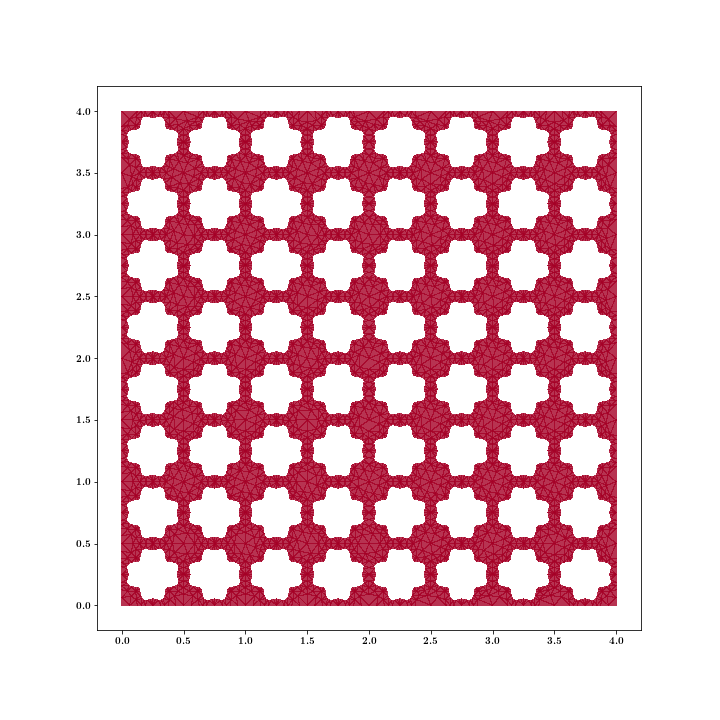
\includegraphics[height=1.1cm, trim={3.5cm 3.5cm 3.5cm 3.5cm}, clip]{lces/figures/rest_pore_01_-01} }}&%
  		{{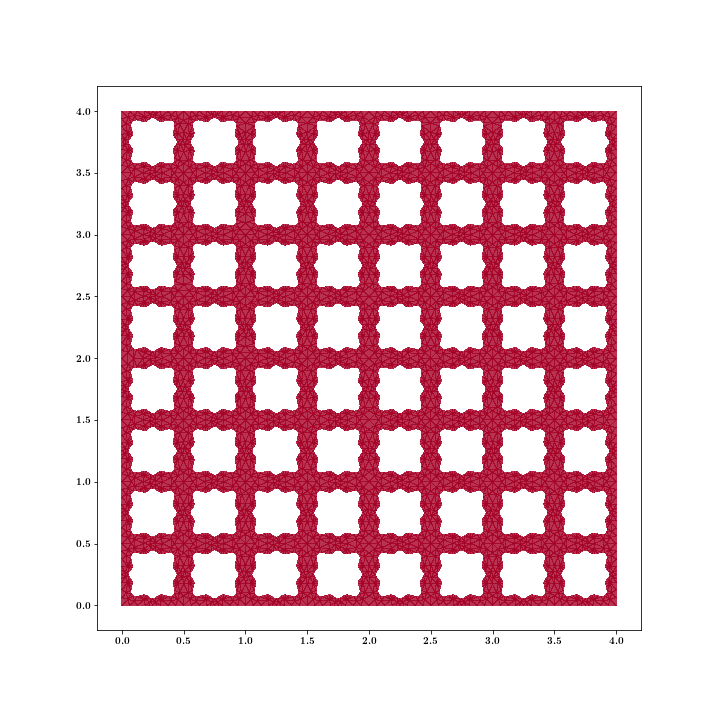
\includegraphics[height=1.1cm, trim={3.5cm 3.5cm 3.5cm 3.5cm}, clip]{lces/figures/rest_pore_-01_01} }}\\\hline
  	\rule{0pt}{7ex}
{{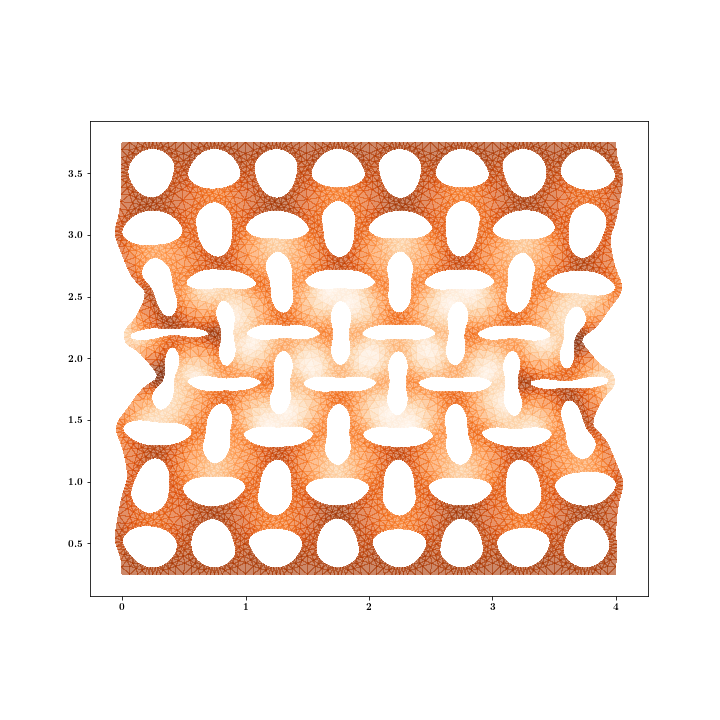
\includegraphics[height=0.95cm, trim={3.5cm 4.5cm 3.5cm 4.5cm}, clip]{lces/figures/pore_0} }}&%
  		{{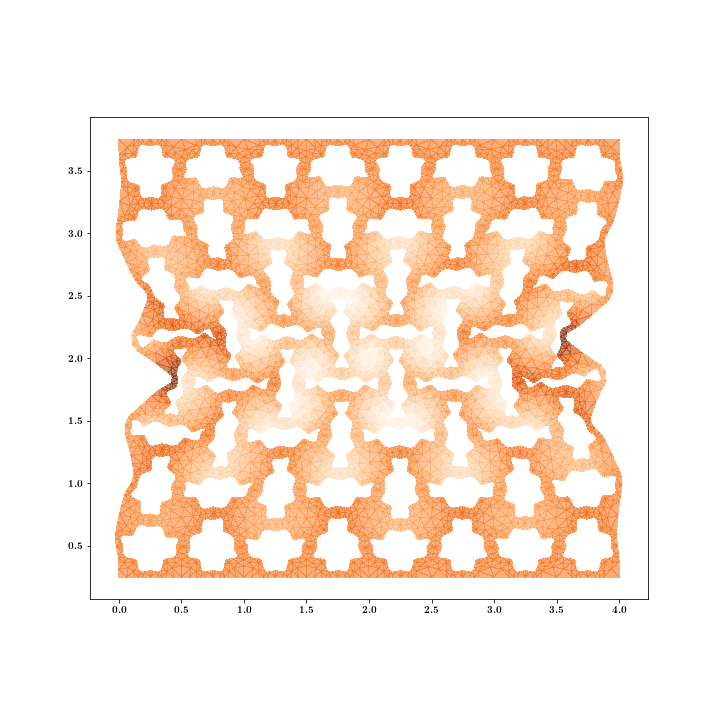
\includegraphics[height=0.95cm, trim={3.5cm 4.5cm 3.5cm 4.5cm}, clip]{lces/figures/pore_01_-01} }}&%
  		{{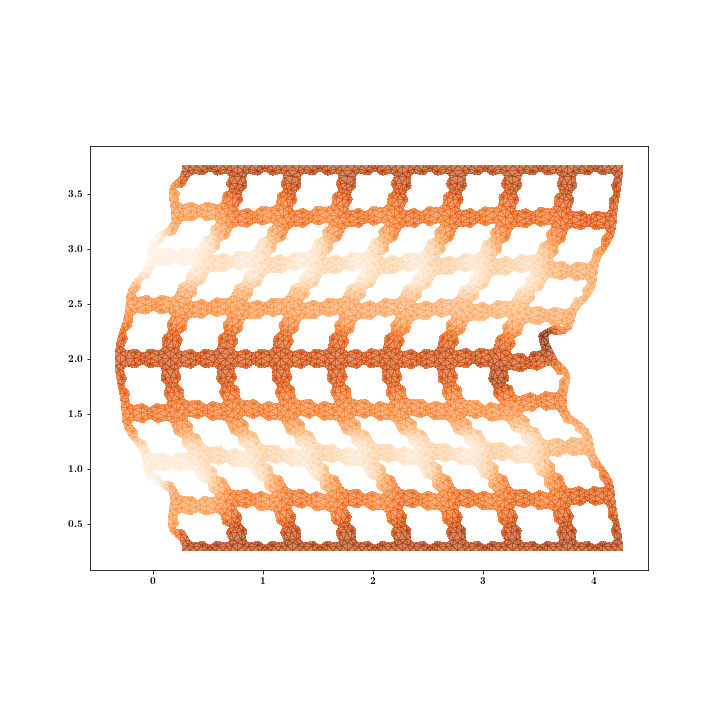
\includegraphics[height=0.9cm, trim={3.5cm 6cm 3.5cm 6cm}, clip]{lces/figures/pore_-01_01} }}%
  	\end{tabular}
  		\vspace{-0.2cm}%
  		\caption{\small Cellular meta-materials. Top: at rest. Bottom: under compression, exhibiting periodic instability varying with pore shape. The left two structures exhibit negative Poisson's ratio, which does not occur in nature.}%
  		\label{Fig:mms}%
\vspace{-0.4cm}
\end{wrapfigure}
Meta-materials hold promise for modern engineering design but are challenging to simulate as the microstructure necessitates a very fine finite element mesh, and as the nonlinear response makes them difficult to approximate with a macroscopic material model.
Most work on meta-materials has relied on engineers and scientists to hand-design materials, rather than numerically optimizing substructure to maximize some objective \citep{ion2016metamaterial}.

We focus on building surrogate models for the two-dimensional cellular solids investigated in \citet{overvelde2014relating}.
These meta-materials consist of square ``cells'' of elastomer, each of which has a pore in its center.
The pore shapes are defined by parameters~$\alpha$ and~$\beta$ which characterize the pore shape in polar coordinates:~${r(\theta) = r_0[1 + \alpha \cos(4\theta) + \beta \cos(8\theta)]}$.
The parameter $r_0$ is chosen such that the pore covers half the cell's volume:~${r_0 = \nicefrac{L_0}{\sqrt{\pi(2 + \alpha^2 + \beta^2}}}$. Constraints are placed on~$\alpha$ and~$\beta$ to enforce a minimum material thicknesses and ensure that $\min_\theta r(\theta) > 0$ as in \citet{overvelde2014relating}.

These pore shapes give rise to complicated nonlinear elastic behavior, including negative Poisson's ratio and double energy wells (i.e., stored elastic energy which does not increase monotonically with strain).
Realizations of this class of materials are shown under axial strain in Figure \ref{Fig:mms}. The continuum mechanics behavior of these elastomer meta-materials can be captured by a neo-Hookean energy model \citep{ogden1997non}.
Let~${X \in \mathbb{R}^d}$, where~${d\leq 3}$ in physical problems, be a point in the resting undeformed material reference configuration, and~$u(X)$ be the displacement of this point from reference configuration. The stored energy in a neo-Hookean solid is
%\begin{equation}
~${E = \int_{\Omega} W(u) dX\,,}$
%\end{equation}
where $W(u)$ is a scalar energy density over $\Omega$, defined for bulk and shear moduli~$\mu$ and~$\kappa$ as:
\begin{equation}\label{eq:neohookean}\small
   W = \frac{\mu}{2} \Big( (\det F)^{-2/d} \text{tr}(FF^T) - d\Big) + \frac{\kappa}{2} (\det F - 1)^2
\end{equation}
where $F$ is the deformation gradient,~${F(X) = \frac{\partial u(X)}{\partial X} + I\,.}$
Pores influence the structure of these equations by changing the material domain $\Omega$.
These solids can be simulated by solving:
\begin{equation}\label{eq:cm}\small
    \text{Div } S = 0 \quad X \in \Omega
\end{equation} \vspace{-0.4cm}
\begin{equation}\label{eq:bc}\small
    G(u) = 0 \quad X \in \partial \Omega
\end{equation}
where~${S = \frac{\partial W}{\partial F}}$ is known as the first Piola-Kirchoff stress, and where Eq.~\ref{eq:bc} defines a boundary condition.
E.g.~${G(u) = u - u_b}$ is a Dirichlet boundary condition; in our case, an externally imposed displacement. ${G(u) = \frac{\partial W}{\partial u} - f_b}$ corresponds to an external force exerting a pressure on the boundary.

To simulate these meta-materials, Eq.~\ref{eq:cm} is typically solved via finite element analysis.
Solving with large meta-material structures is computationally challenging due to fine mesh needed to capture pore geometry and due to the nonlinear response induced by buckling under large displacements.

Solving the PDE in Eq.~\ref{eq:cm} corresponds to finding the~$u$ which minimizes the stored energy in the material subject to boundary conditions.
That is, Eqs.~\ref{eq:cm} and~\ref{eq:bc} may be equivalently be expressed in an energy minimization form:
\begin{equation}\label{eq:cm-energy}\small
    		u = \argmin \int_{X \in \Omega}  W(u) dX \quad \quad\text{subject to } G(u) = 0 \in \partial\Omega
\end{equation}
We use this form to learn surrogates which solve the PDE in a reduced basis of cell boundaries.

\begin{wrapfigure}[12]{r}{0.28\linewidth}
\vspace{-1cm}
\centering
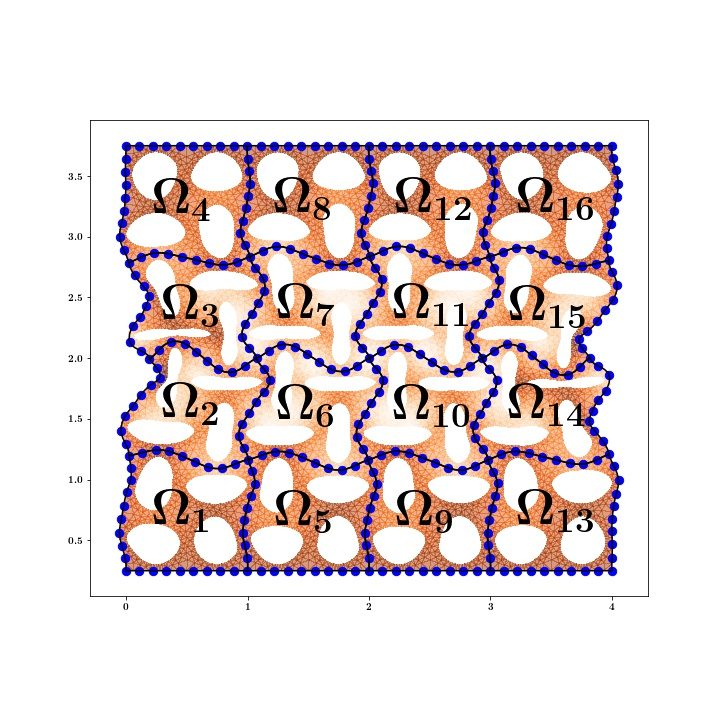
\includegraphics[height=2.7cm, trim={4.0cm 5cm 3.5cm 4.5cm}, clip]{lces/figures/decomp}
	\caption{\small Meta-material domain $\Omega$, partitioned into $\Omega_1$ to $\Omega_{16}$.
	Black lines show $\mathcal{B}$.
	Blue points are control points of splines used to represent $\tilde{u}$.\vspace{-.5cm}}
	\label{Fig:decomp}
\vspace{-.5cm}
\end{wrapfigure}

\section{Composable energy surrogates}
\label{sec:surrogates}
We apply the idea of learning collapsed objectives to the problem of simulating two-dimensional cellular mechanical meta-material behavior.
The material response is determined by the displacement field $u$ which minimizes the energy~${\int_{\Omega} W dX}$, subject to boundary conditions.
We divide $\Omega$ into regular square subregions $\Omega_i$, which we choose to be cells with $2\times2$ arrays of pores, and denote the intersection of the subregion boundaries with~${\mathcal{B} = \partial\Omega_1 \cup \partial\Omega_2 \cup} \dots$
We let $u_i$ be the restriction of $u$ to $\Omega_i$.
We take the quantity of interest to be $u_{\mathcal{B}}$, the restriction of $u$ to $\mathcal{B}$, and the nuisance variables to be the restriction of $u$ to~${\Omega}$\textbackslash~${\mathcal{B}}$.
The partitioning of $\Omega$ is shown in Figure \ref{Fig:decomp}.

The total energy decomposes as a sum over regions:
\begin{align*}
    E(u) = \int_{X \in \Omega} W(u) dX \quad \quad = \sum_i \int_{X \in \Omega_i} W(u_i) dX := \sum_i E(u_i)
\end{align*}\vspace{-0.1cm}
Let $\tilde{u}_i$ be the restriction of $u$ to $\partial\Omega_i$. Note~${\partial\Omega_i = \mathcal{B} \cap \Omega_i}$.
Let the collapsed component energy be:
\begin{align*}
    \tilde{E}_i (\tilde{u}_i) := \min_{u_i} E (u_i) \quad \text{subject to } u_i(X) = \tilde{u}_i(X)\quad X \in \partial{\Omega_i}\,.
\end{align*}
This quantity is the lowest energy achievable by displacements of the \emph{interior} of the cell~$\Omega_i$, given the boundary conditions specified by~$\tilde{u}_i$ on~$\partial{\Omega_i}$.
$\tilde{E}_i(\tilde{u}_i)$ depends on the shape of the region $\Omega_i$, i.e., on the geometry of the pores.
Rather than each possible pore shape having a unique collapsed energy function, we introduce the pore shape parameter~${\xi = (\alpha, \beta)}$ as an argument, replacing~$\tilde{E}_i(\tilde{u_i})$ with~$\tilde{E}(\tilde{u}_i, \xi_i)$.
The macroscopic behavior of the material is fully determined by this \emph{single} collapsed energy function~${\tilde{E}(\tilde{u}_i, \xi_i)}$.
Given the true collapsed energy functions, we could accurately simulate material behavior in the reduced basis of the boundaries between each component~$\Omega_i$.\footnote{So long as forces and constraints are only applied on $\mathcal{B}$.}

We learn to approximate this collapsed energy function from data. This function may be duplicated and composed to simulate the material in the reduced basis~$\mathcal{B}$, an approach we term \emph{composable energy surrogates} (CESs).
A single CES is trained to approximate the function $\tilde{E}$ by fitting to supervised data~${(\tilde{u}_i, \xi_i, \tilde{E}(\tilde{u}_i, \xi_i))}$, where $\xi_i$ and $\tilde{u}_i$ may be drawn from any distribution corresponding to anticipated pore shapes and displacements, and the targets $\tilde{E}(\tilde{u}_i, \xi_i)$ are generated by solving the PDE in a small region $\Omega_i$ with geometry defined by $\xi_i$ and with $\tilde{u}_i$ imposed as a boundary condition.
This CES may be used to approximate the energy in multiple spatial locations: it may be "composed" to approximate the total energy of larger cellular meta-materials.

To efficiently solve for a reduced-basis displacement~$u_{\mathcal{B}}$ on~$\mathcal{B}$,
we minimize the composed surrogate energy,~${\hat{E}(u_\mathcal{B}) = \sum_i \hat{E}(\tilde{u}_i, \xi_i)}$, where~$\hat{E}(\tilde{u}_i, \xi_i)$ is the model's
prediction of $\tilde{E}(\tilde{u}_i, \xi_i)$, the collapsed energy of one component.
Training CES which produce accurate reduced-basis solutions may
be thought of as a highly-structured imitation learning problem.
A sufficient condition for finding the correct minimum is for the "action" taken by the surrogate---the derivative of the energy approximation~${\nabla_{u_{\mathcal{B}}} \hat{E}}$---to match the "action" taken by an expert---the \emph{total} derivative,~${\nabla_{u_{\mathcal{B}}} \min_{u\notin \mathcal{B}} E(u)}$---along the optimization trajectory.
If so, the surrogate will follow the trajectory of a valid, if non-standard, bilevel gradient-based procedure for minimizing the energy, corresponding to (\ref{eq:bilevel}). Given an imperfect surrogate, the error in the final solution will depend on
the error in approximating~${\nabla_{u_{\mathcal{B}}} \min_{u\notin \mathcal{B}} E(u)}$
with $\nabla_{u_{\mathcal{B}}} \hat{E}$ along the trajectory.
This observation informs our model, training, and data collection procedures, described in the following sections.
%\setlength{\abovedisplayskip}{6pt}
%\setlength{\belowdisplayskip}{5pt}
\section{Model architecture}
\label{sec:model}
Our CESs take the form of a neural architecture, designed to respect known properties of the true potential energy and to maximize usefulness as surrogate energy to be minimized via a gradient-based procedure.
The effects of these design choices are quantified via an ablation study in the appendix.

\textbf{Reduced-basis parameterization}.
We use one cubic spline for each horizontal and vertical displacement function along each face of the square, with evenly spaced control points and ``not-a-knot'' boundary conditions.
Our vector representation of $\tilde{u}$ is~${\rvu \in \mathbb{R}^{2n}}$, formed from the horizontal and the vertical displacement values at each of the $n$ control points.
Splines on adjacent faces share a control point at the corner. Using $N$ control points to parameterize the function along each face requires~${n = 4*(N-1)}$ control points to parameterize a $1d$ function around a single cell.
For all experiments we use~${N = 10}$ control points along each edge, resulting in~${\rvu \in \mathbb{R}^{72}}$.

\textbf{Model structure and loss}. Our model structure and losses are shown below.
In the energy model $\hat{E}$,
$f_\phi$ is a neural network with parameters $\phi$ and $\mathcal{R}$ removes rigid-body rotation and translation.
Our loss function is~${\mathcal{L} =  \mathcal{L}^0 + \mathcal{L}^1 + \mathcal{L}^2\,,}$
which is a weighted sum of losses on the $0$th, $1$st and $2$nd energy derivatives.
$\nabla_{\rvu}$ and $\nabla^2_{\rvu}$ are the gradient and Hessian of the surrogate energy $\hat{E}$ or the ground-truth energy $\tilde{E}$ with respect to $\rvu$, and $v$ is sampled independently for each training example in a batch.
\small
\begin{align*}
    \hat{E}(\rvu, \xi) = \underbrace{||\mathcal{R}(\rvu)||_2^2}_\text{Linear elastic component} \underbrace{\exp \{f_\phi \big(\mathcal{R}(\rvu), \xi\big)\}}_\text{Stiffness}\,,\quad \quad
    \mathcal{L}^0 = \underbrace{\left\lVert f_\phi \big(\mathcal{R}(\rvu), \xi\big) - \log \frac{\tilde{E}(\tilde{u})}{||\mathcal{R}(\rvu)||_2^2} \right\rVert_2^2}_\text{Log-stiffness loss}\,, \\
    \mathcal{L}^1 = \underbrace{1 - \frac{\langle \nabla_{\rvu} \hat{E}, \nabla_{\rvu} \tilde{E}\rangle}{||\nabla_{\rvu} \hat{E}|| ||\nabla_{\rvu} \tilde{E}||}}_\text{Cosine distance between gradients}\,,\quad \quad
    \mathcal{L}^2 = \underbrace{1 - \frac{\langle \nabla^2_{\rvu} \hat{E} v,  \nabla^2_{\rvu} \tilde{E} v \rangle}{||\nabla^2_{\rvu} \hat{E} v|| ||\nabla^2_{\rvu} \tilde{E} v||}}_{\substack{\text{Cosine distance between}\\\text{Hessian-vector products}}} \quad \underbrace{v \sim \mathcal{N}(0, I^{2n})}_\text{Projection vector for Hessian}\,.
\end{align*}\normalsize
\textbf{Invariance to rigid body transforms}.
The true elastic energy is invariant to rigid body transforms of a solid.
This invariance may be hard to learn exactly from data. We use a module $\mathcal{R}$ which applies \emph{Procrustes analysis}, i.e. finds and applies the rigid body transform which minimizes the Euclidean distance to a reference (we use the rest configuration). This is differentiable and closed-form.

\textbf{Encoding a linear elastic bias}.
The energy is approximated well by a linear elastic model when at rest:~${\tilde{E}^i(\tilde{u}_i) \approx \mathcal{R}(\rvu_i)^T A^i \mathcal{R}(\rvu_i)}$ for a stiffness matrix~$A^i$ depending on~$\xi_i$.
We scale our net's outputs by~$||\mathcal{R}(\rvu_i)||_2^2$ so that it needs only capture a ``scalar stiffness''~$\nicefrac{E}{||\mathcal{R}(\rvu_i)||_2^2}$ accounting for the geometry of~$A^i$ given~$\xi_i$ and for deviation from the linear elastic model.

\textbf{Parameterizing the log-stiffness}.
The energy of a component $\tilde{E}^i(u_{0, i})$ is nonnegative, and the ratio of energy to a linear elastic approximation varies over many orders of magnitude.
We parameterize the log of the scalar stiffness with our neural network $f_\phi$ rather than the stiffness.

\textbf{Log-stiffness loss}. We wish to find neural network parameters $\phi$ which lead to accurate energy predictions for many different orders of magnitude of energy and displacement.
Minimizing the~$\ell^2$ loss between predicted and true energies penalizes errors in predicting large energies more than proportional errors predicting small energies.
Instead, we take the~$\ell^2$ loss between the predicted log-stiffness~$f_\phi (\mathcal{R}(\rvu), \xi)$ and the effective ground-truth log-stiffness,~$\log\nicefrac{ \tilde{E}(\tilde{u})}{||\mathcal{R}(\rvu)||_2^2}$.

\textbf{Sobolev training with gradients and Hessian-vector products}.
"Sobolev training" on derivatives of a target function can aid generalization \citep{czarnecki2017sobolev}.
Accuracy of CES' derivatives is crucial, so we Sobolev train on energy gradients and Hessians.
We obtain ground-truth gradients cheaply via the adjoint method \citep{lions1971optimal}. Given a solution $u_i$ to the PDE in $\Omega_i$ with boundary conditions $\tilde{u}_i$, the gradient~${\nabla_{\tilde{u}_i} \tilde{E}_i(\tilde{u}_i)}$ requires solving a linear system with the same cost as one Newton step of solving the PDE \citep{mitusch2019dolfin}.
The spline is a linear map $\mathcal{M}$ from $\rvu_i$ to $\tilde{u}_i$ in the finite element basis, so~${\nabla_{\rvu_i} \tilde{E}_i(\tilde{u}_i) = \mathcal{M}^T \nabla_{\tilde{u}_i} \tilde{E}_i(\tilde{u}_i)}$. The surrogate gradient,~${\nabla_{\rvu_i} \hat{E}_\phi(\rvu_i, \xi_i)}$,
is computed with one backward pass. Given solution and gradient, we compute $\nabla^2_{\rvu}\tilde{E}$
with one linear solve per entry of $\rvu$. As $\rvu \in \mathbb{R}^{72}$ and many more than 72 Newton steps are usually needed to solve the PDE, this does not dominate the cost of data collection.
Computing the full Hessian of the surrogate energy,~${\nabla^2_{\rvu_i}\hat{E}_\phi(\rvu_i, \xi_i)}$, would require $2n$ backward passes.
Instead we train on Hessian-vector products, which require only one additional backward pass.

\textbf{Cosine distance loss for Sobolev training}.
Energy gradient and Hessian values vary over many orders of magnitude, with
higher energies leading to larger derivatives.
We wish our model to be accurate across a range of operating conditions.
Rather than placing an~$\ell^2$ loss on the gradient and Hessian-vector products as in \citet{czarnecki2017sobolev}, we minimize the cosine distance between ground truth and approximate gradients and Hessians, which is naturally bounded in $[0, 1]$.
%\vspace{-0.5cm}

\vspace{-0.1cm}\section{Data and training}\label{sec:training}\vspace{-0.1cm}
Data collection has two phases.
First, we collect training and validation datasets using Hamiltonian Monte Carlo \citep{duane1987hybrid} to preferentially sample displacements which correspond to lower energy modes.
Next, we perform dataset aggregation \citep{ross2011reduction} to augment the dataset so that the surrogate will be accurate
on states encountered when deployed.
We provide details of the hardware and the software packages used in the appendix.

\textbf{Solving the PDE}.
To collect training data, we use the reduced-basis displacement $\tilde{u}$ corresponding to a vector of spline coefficients $\rvu$ as the boundary condition around a domain $\Omega$ representing a $2\times2$-pore subdomain, and solve the PDE using a load-stepped relaxed Newton's method \citep{sheng2002automatic}. The relaxed Newton's method takes the iteration~${\vec{u} \leftarrow \vec{u} - \lambda
(\frac{\partial^2 E}{\partial \vec{u}^2})^{-1}\frac{\partial E}{\partial \vec{u}}}$.
Here, $0 < \lambda < 1$ is the relaxation parameter (analogous to a step size), and $\vec{u}$ is the vector of coefficients defining $u$ in the FEA basis.
Newton's method requires an initial guess which is sufficiently close to the true solution \citep{kythe2004introduction}.
Smaller relaxation parameters yield a greater radius of convergence but necessitate more steps to solve the PDE.

The radius of convergence can also be aided by load-stepping: solving the PDE for a sequence of boundary conditions, annealing from an initial boundary condition for which we have a good initial guess (e.g., the rest configuration) to a final boundary condition~$\tilde{u}$, using the solution to the previous problem as an initial guess for Newton's method for the next problem.
We find that combining load stepping with a relaxed Newton's method is more efficient than using either alone.
Except where specified, we linearly anneal from rest to~$\tilde{u}$ over~$10$ load steps and use a relaxation parameter~$\lambda = 0.1$.

\textbf{Initial dataset collection}.
We wish to train on varied displacement boundary conditions. As solution procedures minimize energy, lower energy modes will be encountered in the solve. We choose a distribution with density the product of a Boltzmann density~$\exp \{\tilde{E}\}/Z$ and a Gaussian density~$\mathcal{N}(\bar{x}(\rvu); \bar{\mu}, \Sigma)$, where~${\bar{x}(\rvu) \in \mathbb{R}^{2\times2}}$ is a macroscopic strain tensor\footnote{See the appendix for approximating $\bar{x}$ from $\rvu$.} corresponding to $\rvu$,
$\bar{\mu}$ is a target strain drawn from an i.i.d.\ Gaussian with standard deviation~$0.15$, and~$\Sigma$ is set to~$(\bar{\mu}\circ \bar{\mu})^{-1}$.
%We approximate the macroscopic strain tensor as\\
%\resizebox{\linewidth}{!}{
%  \begin{minipage}{\linewidth}
%\begin{align*}
%\bar{x}(\rvu) = \frac{1}{N} \begin{bmatrix}
%\displaystyle\sum_{X \in \text{rhs}} \!\!u_1(X) \!-\!\!\! \sum_{X \in \text{lhs}} \!\!u_1(x)
%&
%\displaystyle\sum_{X \in \text{rhs}} \!\!u_2(X) \!-\!\!\! \sum_{X \in \text{lhs}} \!\!u_2(X)
%\\
%\displaystyle\sum_{X \in \text{top}} \!\!u_1(X) \!-\!\!\! \sum_{X \in \text{bot}} \!\!u_1(x)
%&
%\displaystyle\sum_{X \in \text{top}} \!\!u_2(X) \!-\!\!\! \sum_{X \in \text{bot}} \!\!u_2(X)
%\end{bmatrix}
%\end{align*}
%\end{minipage}
%}
% Above,~$u_1(X)$ and~$u_2(X)$ are horizontal and vertical displacements defined by $\rvu$ at a point $X$, and top, bot, lhs and rhs are the set of control point locations for the splines on the top, bottom, left and right of the component.

Given a solution to the PDE, the log-density and its displacement may be cheaply computed (the latter via the adjoint method). Making use of these gradients, we sample data points with Hamiltonian Monte Carlo (HMC). After sampling a data point, we compute the corresponding Hessian and save the tuple $(\rvu, \xi, \tilde{E}, \nabla_{\rvu} \tilde{E}, \nabla^2_{\rvu} \tilde{E})$ as a data point.

We initialize each HMC data collector by sampling a macroscopic displacement target and a random pore shape. We do not use load-stepping, instead using the solution for the $\rvu$ used in the previous iteration of HMC's leapfrog integration as an initial guess for solving the PDE. We randomize HMC hyperparameters for each collector to attempt to minimize the impact of specific settings: see the appendix for exact ranges. We sample 55000 training examples and 5000 validation examples altogether. We visualize displacements drawn from this distribution in the appendix.%---in effect, we are sampling hierarchically from a mixture of distributions. The parameter range is chosen such that solving the PDE at each leapfrog step converges in reasonable time. We draw a temperature to scale the log-density from $\mathcal{U}([0.0001, 0.0005, 0.001, 0.005, 0.01, 0.05, 0.1])$, a standard deviation from which to draw an initial Gaussian potential from $\mathcal{U}(0.01, 0.3)$, and a leapfrog integration path length from $\mathcal{U}(0.005, 0.02)$ and step size from $\mathcal{U}(0.05, 0.3)$.

\textbf{Data aggregation}.
Surrogate deployment defies standard i.i.d.\ assumptions in supervised learning.
The deployed surrogate encounters states determined by the energy it defines and by boundary conditions on the composed body. Given a dataset such as that we sampled with HMC, the distribution over states encountered by the surrogate in deployment may be very different to the distribution of states in this dataset.

This problem---that training an agent to predict expert actions can lead to trajectories dissimilar to those on which it was trained---is a central concern in the imitation learning literature. A number of solutions exist \citep{schroecker2017state}.
One is dataset aggregation, or \textsc{DAgger} \citep{ross2011reduction}, which reduces imitation learning or structured prediction to online learning.

In \textsc{DAgger}, a policy is deployed and trajectories are collected.
The expert is queried on the states in these trajectories.
The state-action pairs are appended to the dataset, and the policy is retrained on this dataset.
This process of deployment, querying, appending data, and retraining, is iterated.
The distribution of states encountered in deployment and the distribution of states in the dataset converge. 
Under appropriate assumptions, the instantaneous regret of the learned policy vanishes with the number of iterations, i.e., the learned policy matches the expert policy on its own trajectories.

\citet{ross2011reduction} present \textsc{DAgger} as a method for discrete action spaces.
We have a continuous action space: the gradient of the energy in a cell.
We do not investigate generalizing \textsc{DAgger}'s regret guarantees to continuous action spaces, but the intuition holds that we wish our model to ``imitate'' the finite element ``expert'' on the optimization trajectories the model produces.

We initialize our training data with HMC as described earlier.
We then apply \textsc{DAgger} by iterating: (i) training the surrogate; (ii) composing surrogates and finding displacements which minimize the composed energy; (iii) sampling displacements along the surrogate's solution path, querying the ground-truth energy and energy derivatives using FEA, and adding these new data points to the dataset.
We visualize displacements generated by \textsc{DAgger} in the appendix.
%\vspace{-0.3cm}
\section{Software and hardware}
We implement the finite element models in~\texttt{dolfin}~\citep{logg2010dolfin, logg2012dolfin}, a Python front end to FEniCS \citep{alnaes2015fenics,logg2012automated}. To differentiate through finite element solutions, we use the package~\texttt{dolfin-adjoint}~\citep{mitusch2019dolfin}. We implement surrogate models in PyTorch \citep{paszke2019pytorch}.

We use Ray \citep{moritz2018ray} to run distributed workloads on Amazon EC2. The initial dataset is collected using 80 M4.xlarge CPU spot workers. While training the surrogate, we use a GPU P3.large driver node to train the model, and 80 M4.xlarge CPU spot worker nodes performing \textsc{DAgger} in parallel. These workers receive updated surrogate model parameters, compose and deploy the surrogate, sample displacements along the solution path, query the finite element model for energy and derivatives, and return data to the driver node. Initial dataset collection and model training with \textsc{DAgger} each take about one day in wall-clock time.
%\vspace{-0.3cm}

\section{Empirical evaluation}
\label{sec:results}
We demonstrate the ability of Composable Energy Surrogates (CES) to efficiently produce accurate solutions. We consider the systems constructed in \citet{overvelde2014relating}: structures with an $8\times8$ array of pores, corresponding to a $4\times4$ assembly of our surrogates, each representing a $2\times2$-pore component. We sample pore shapes from a uniform distribution over valid shapes defined in \citet{overvelde2014relating}. For \textsc{DAgger}, we sample vertical axial strain magnitudes from $\mathcal{U}(0., 0.3)$, and apply compression with probability $0.8$ (as compressive displacements involve more interesting pore collapse) or tension with probability $0.2$.

We compare our composed surrogates to finite element analysis with different-fidelity meshes under axial compression and tension with a macroscopic displacement of~$0.125 L_0$, where~$L_0$ is the original length of the solid. See the appendix for details of the finite element meshes. We use seven pore shapes: $\xi=(0, 0)$, corresponding to circular pores, and six $\xi$ sampled from a uniform distribution over pore parameters defined as valid in \citet{overvelde2014relating}.
\begin{figure*}[h]
 \begin{tabular}{cc}
	 {\resizebox{0.45\textwidth}{!}{
 \begin{adjustbox}{clip, trim=.4cm .3cm .7cm .3cm}
	 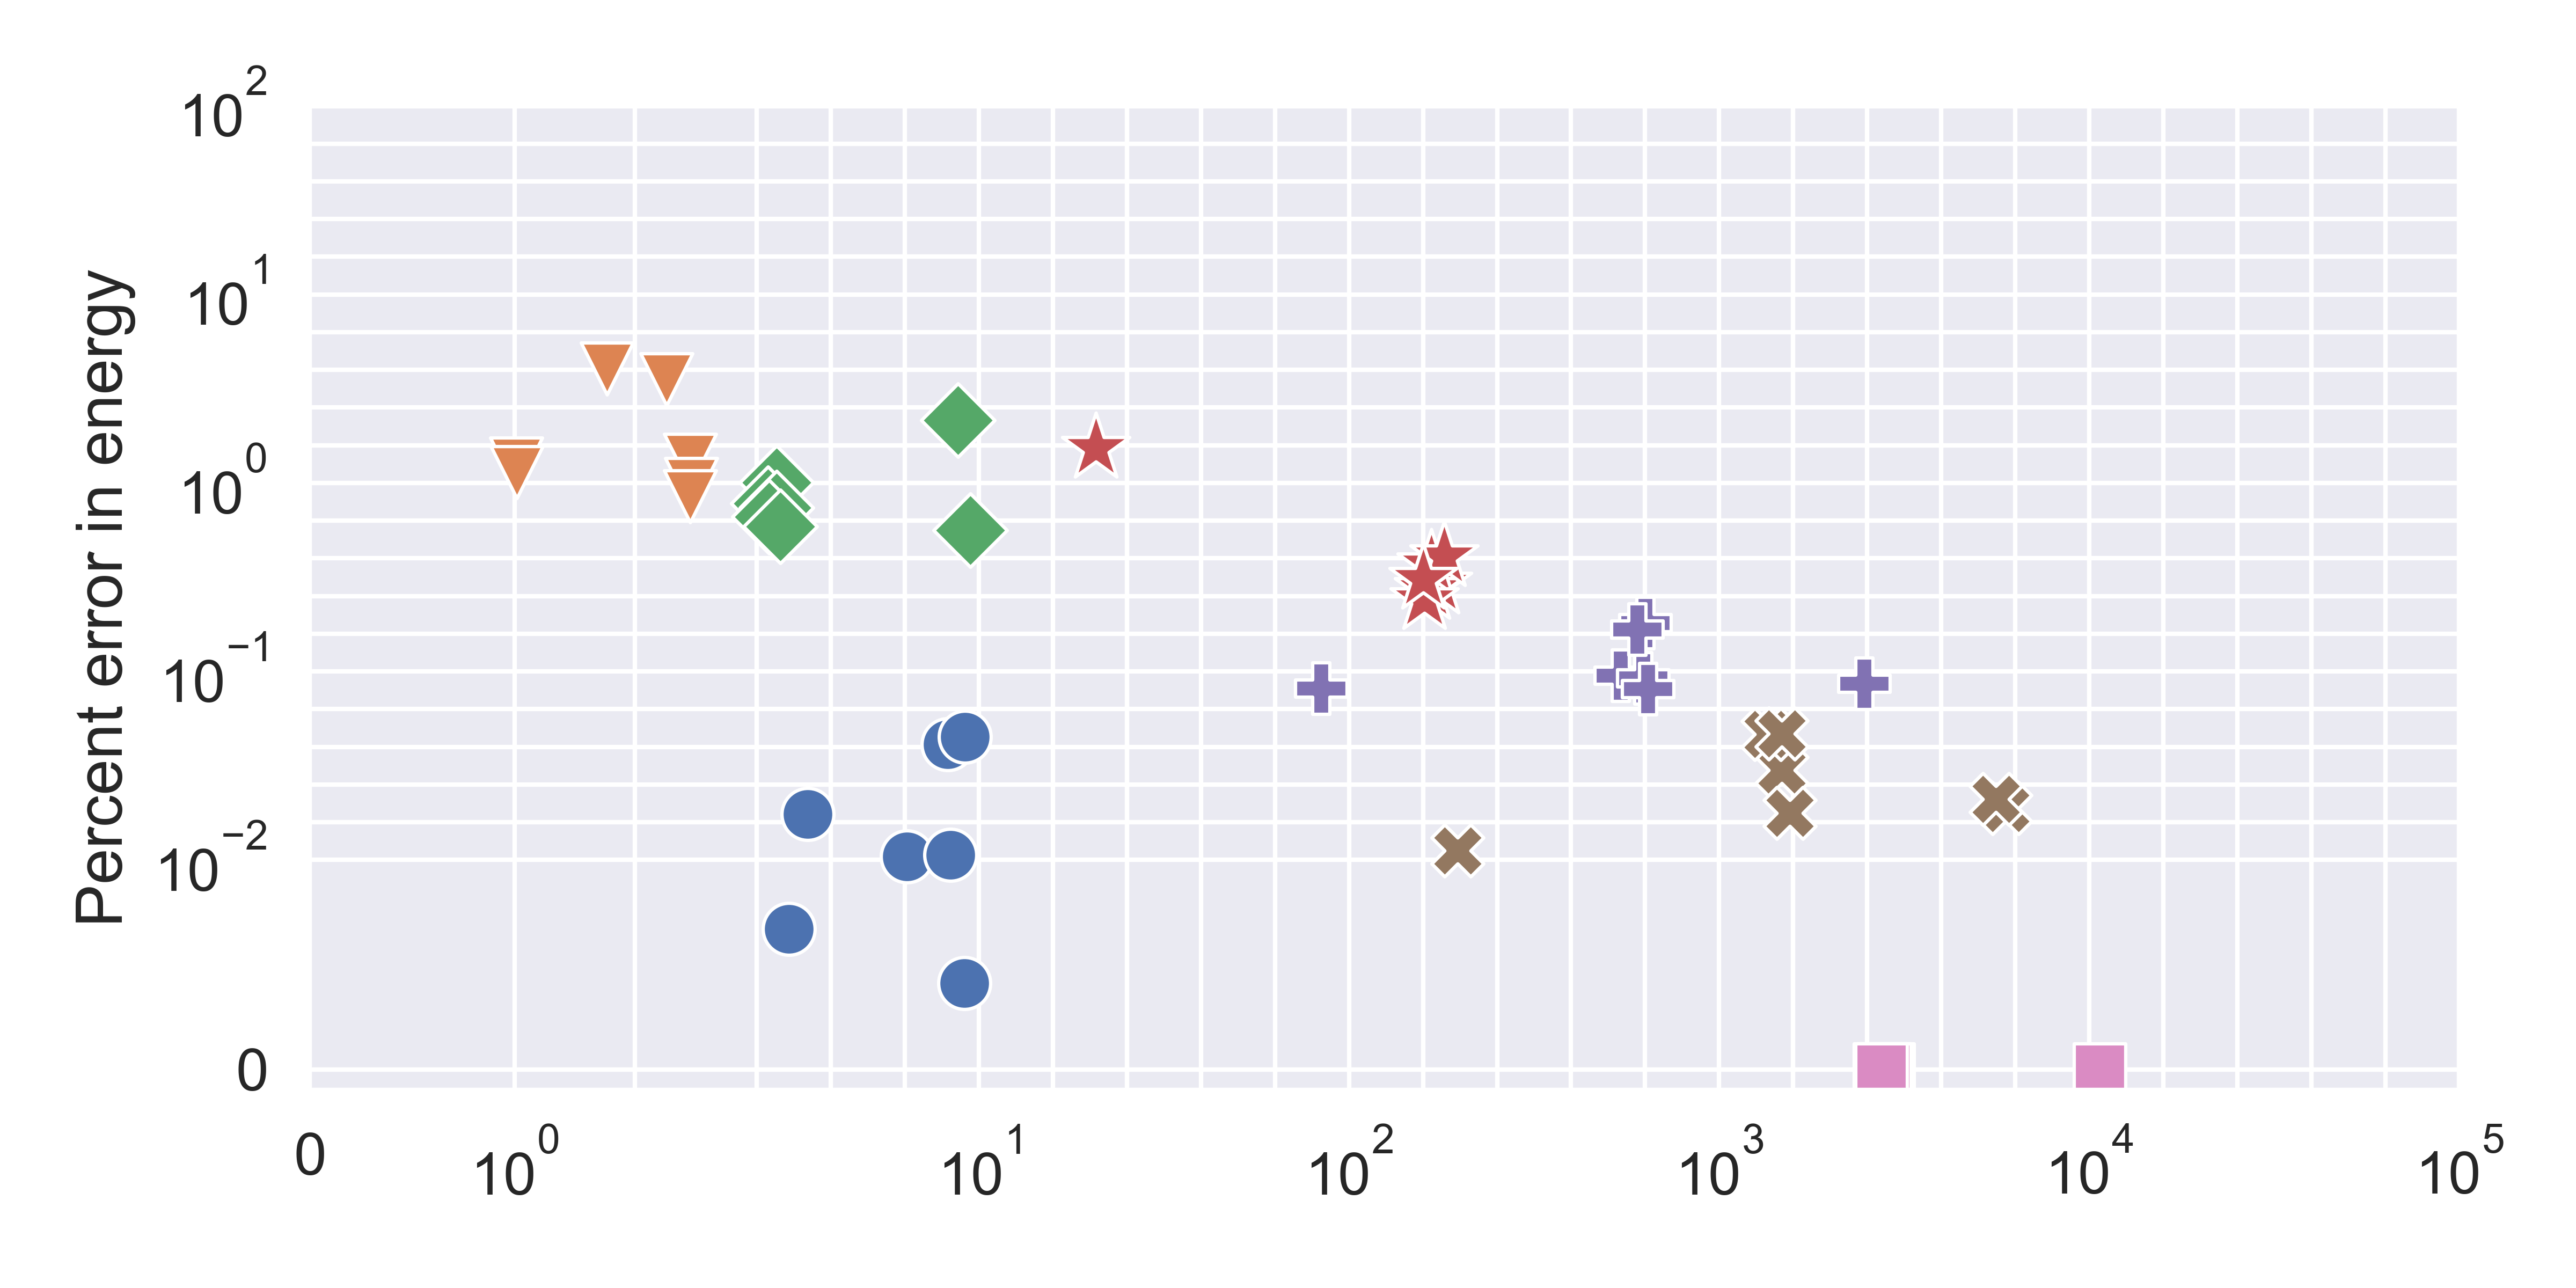
\includegraphics{lces/figures/compression_E.png}
	 \end{adjustbox}
	 }}&
	{\resizebox{0.45\textwidth}{!}{
 \begin{adjustbox}{clip, trim=.4cm .3cm .7cm .3cm}
	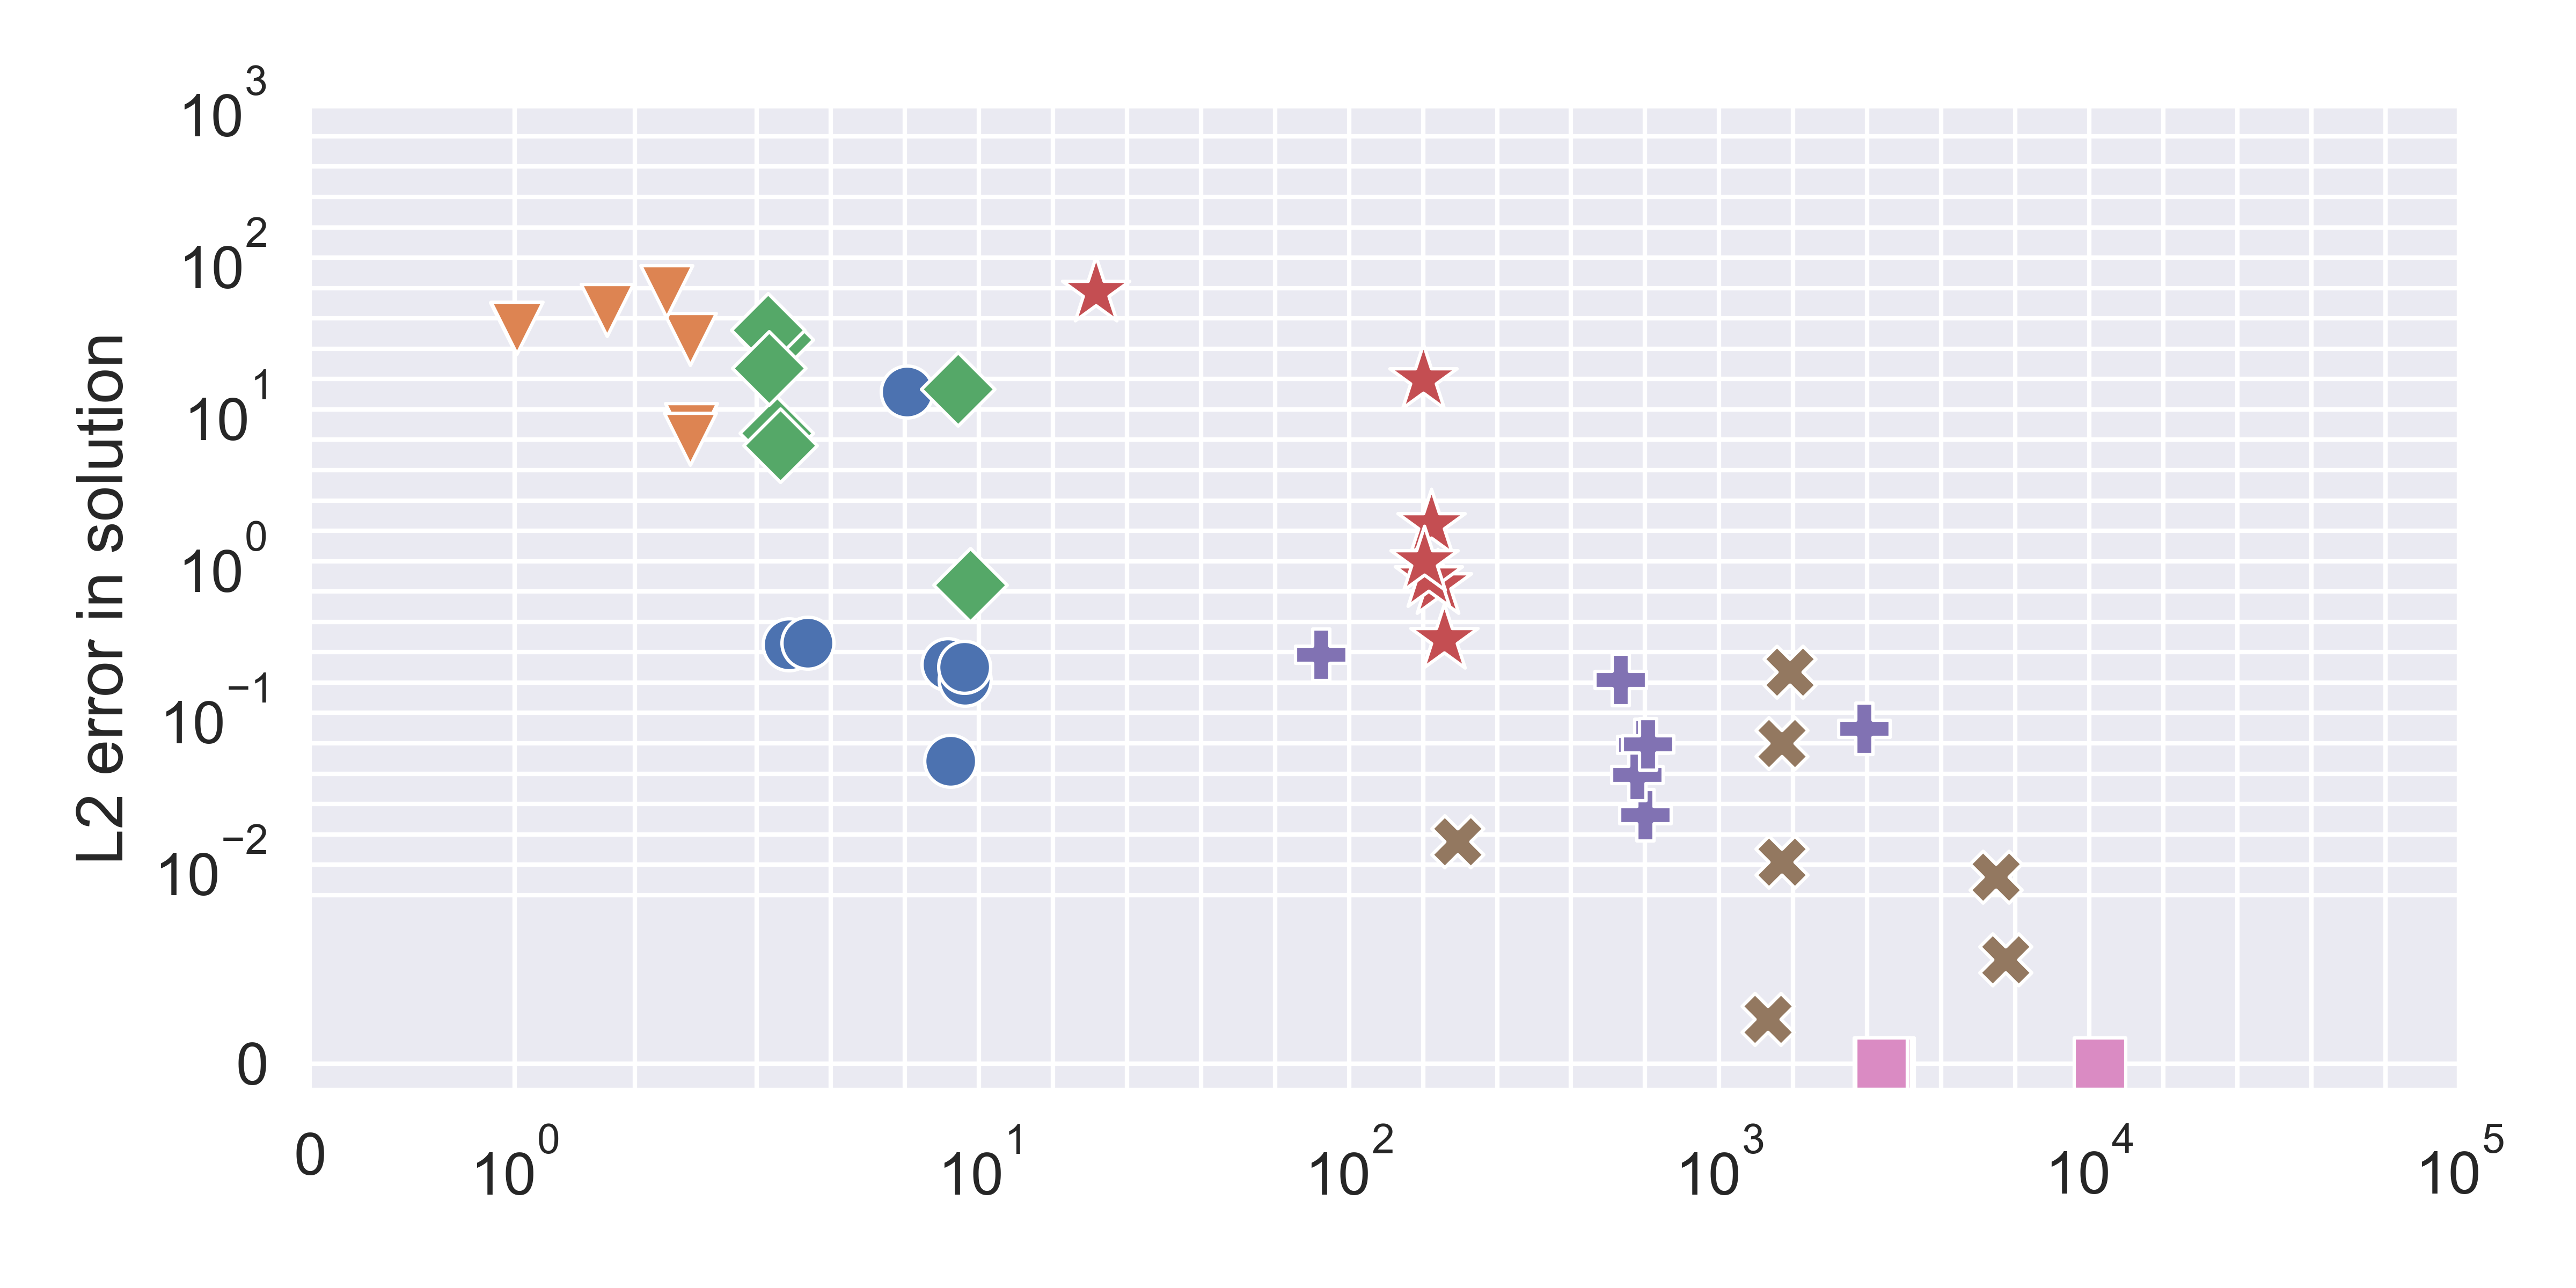
\includegraphics{lces/figures/compression_err.png}
	 \end{adjustbox}
	}}\\
%\rule{0pt}{13ex}
{\resizebox{0.45\textwidth}{!}{
 \begin{adjustbox}{clip, trim=.3cm 0cm .7cm .3cm}
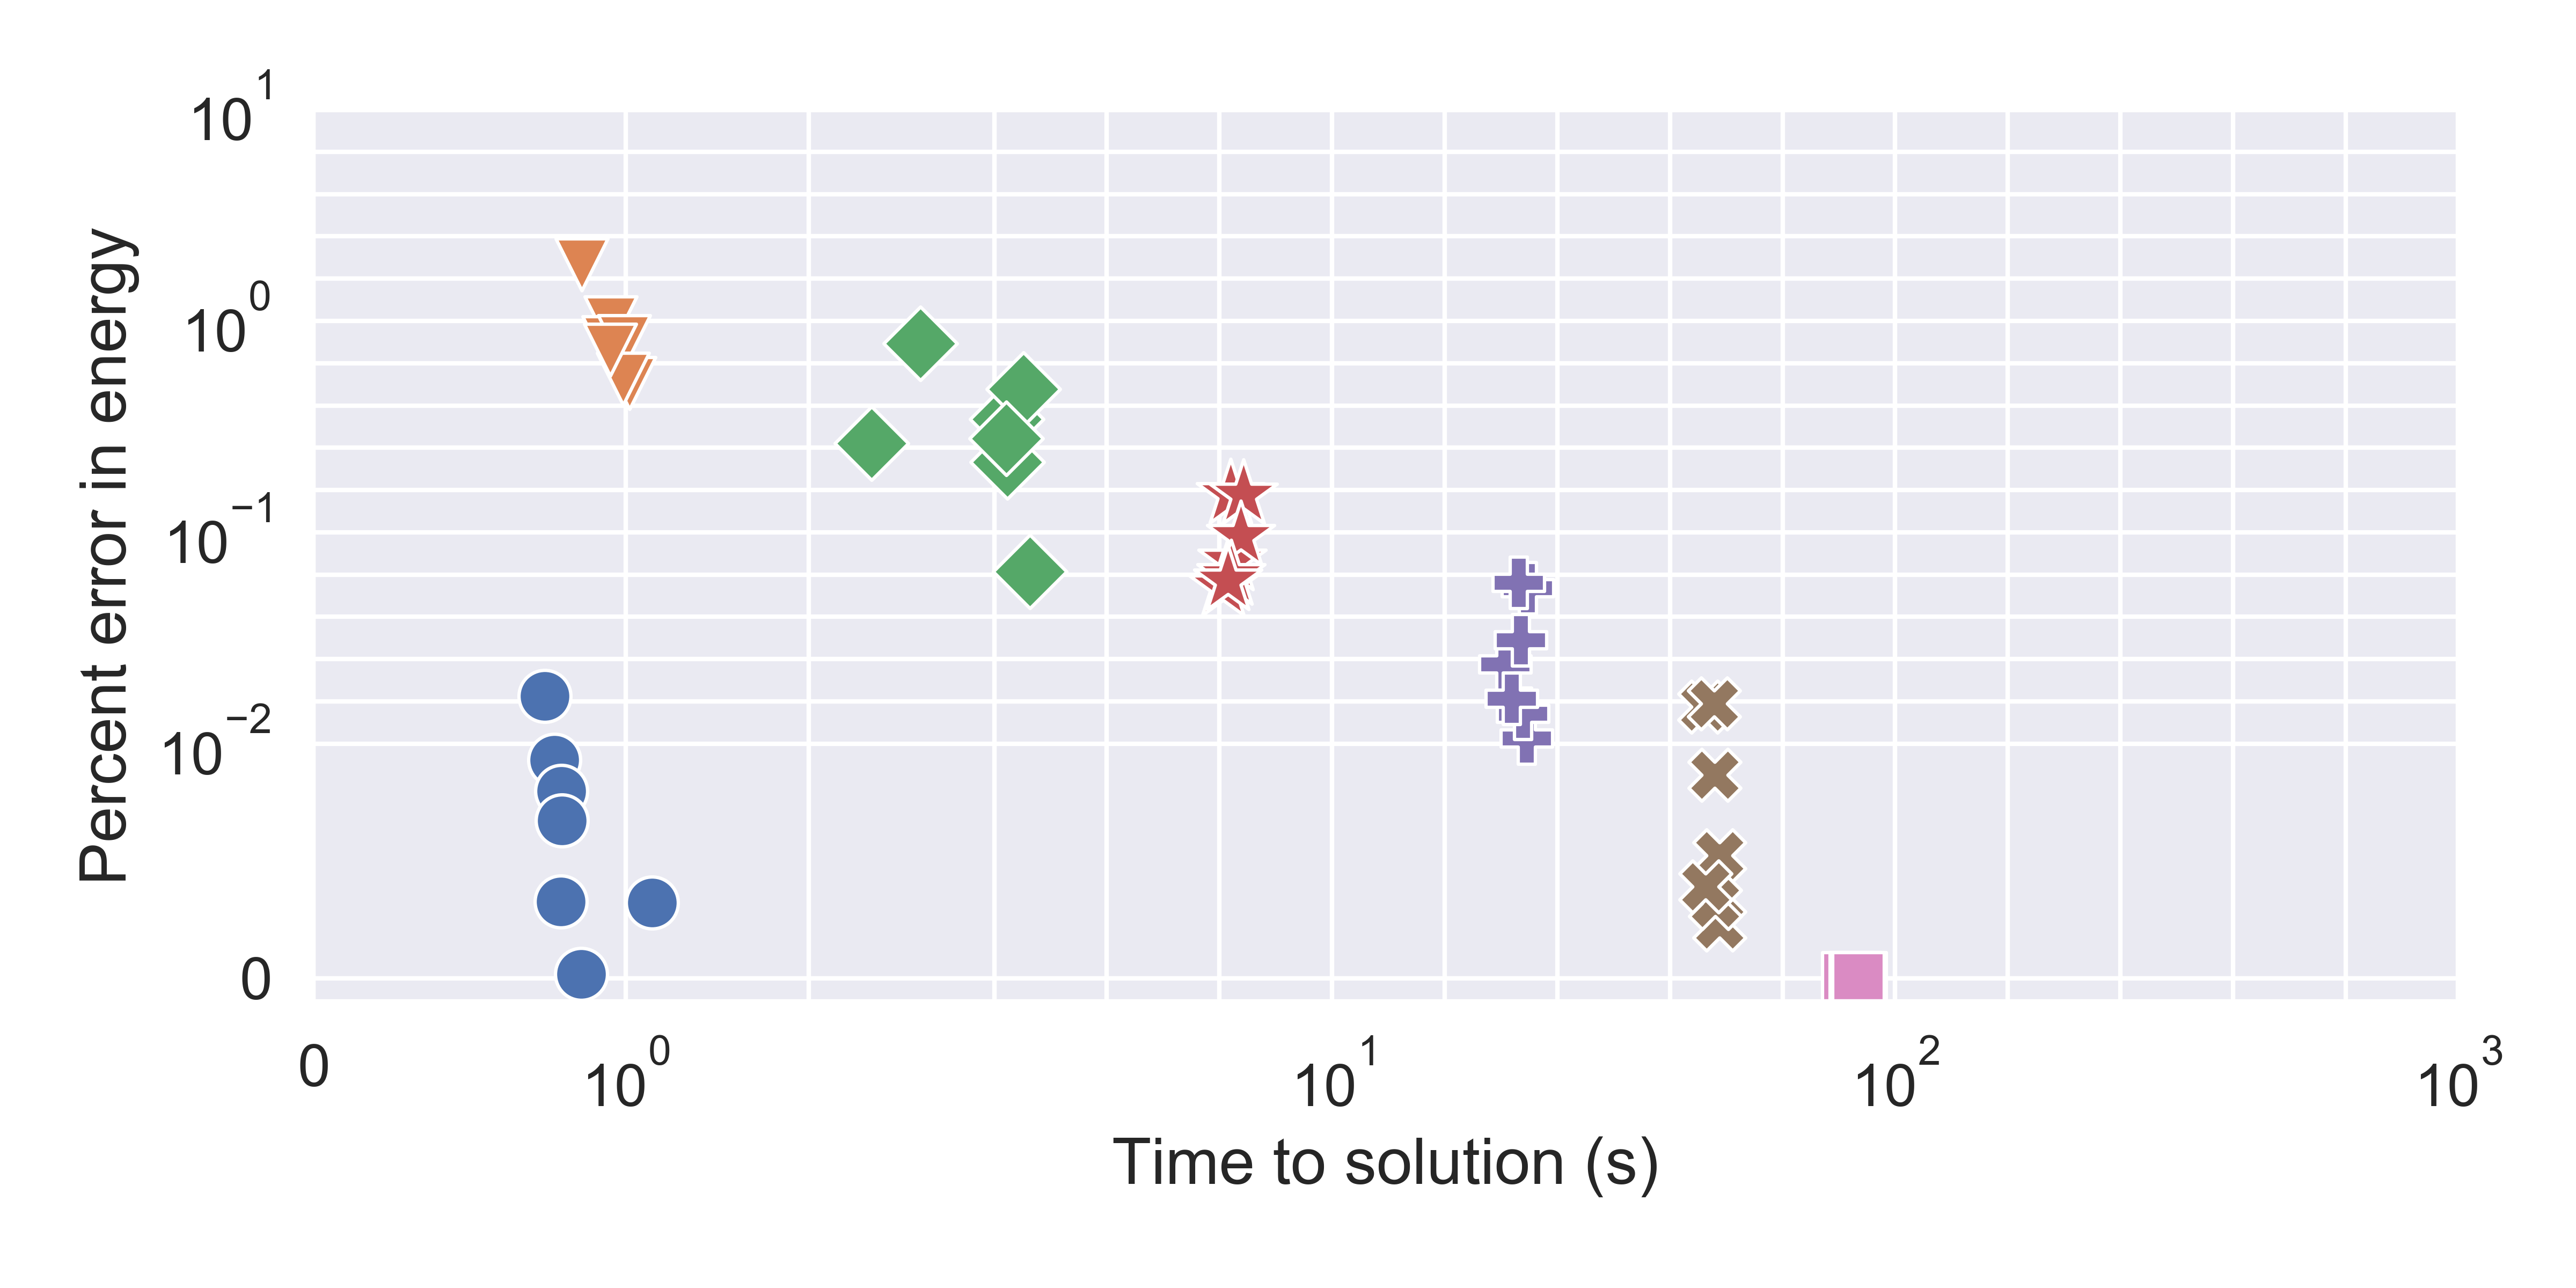
\includegraphics{lces/figures/tension_E.png}
 \end{adjustbox}
}}&%
	{\resizebox{0.45\textwidth}{!}{
 \begin{adjustbox}{clip, trim=.3cm 0cm .7cm .3cm}
	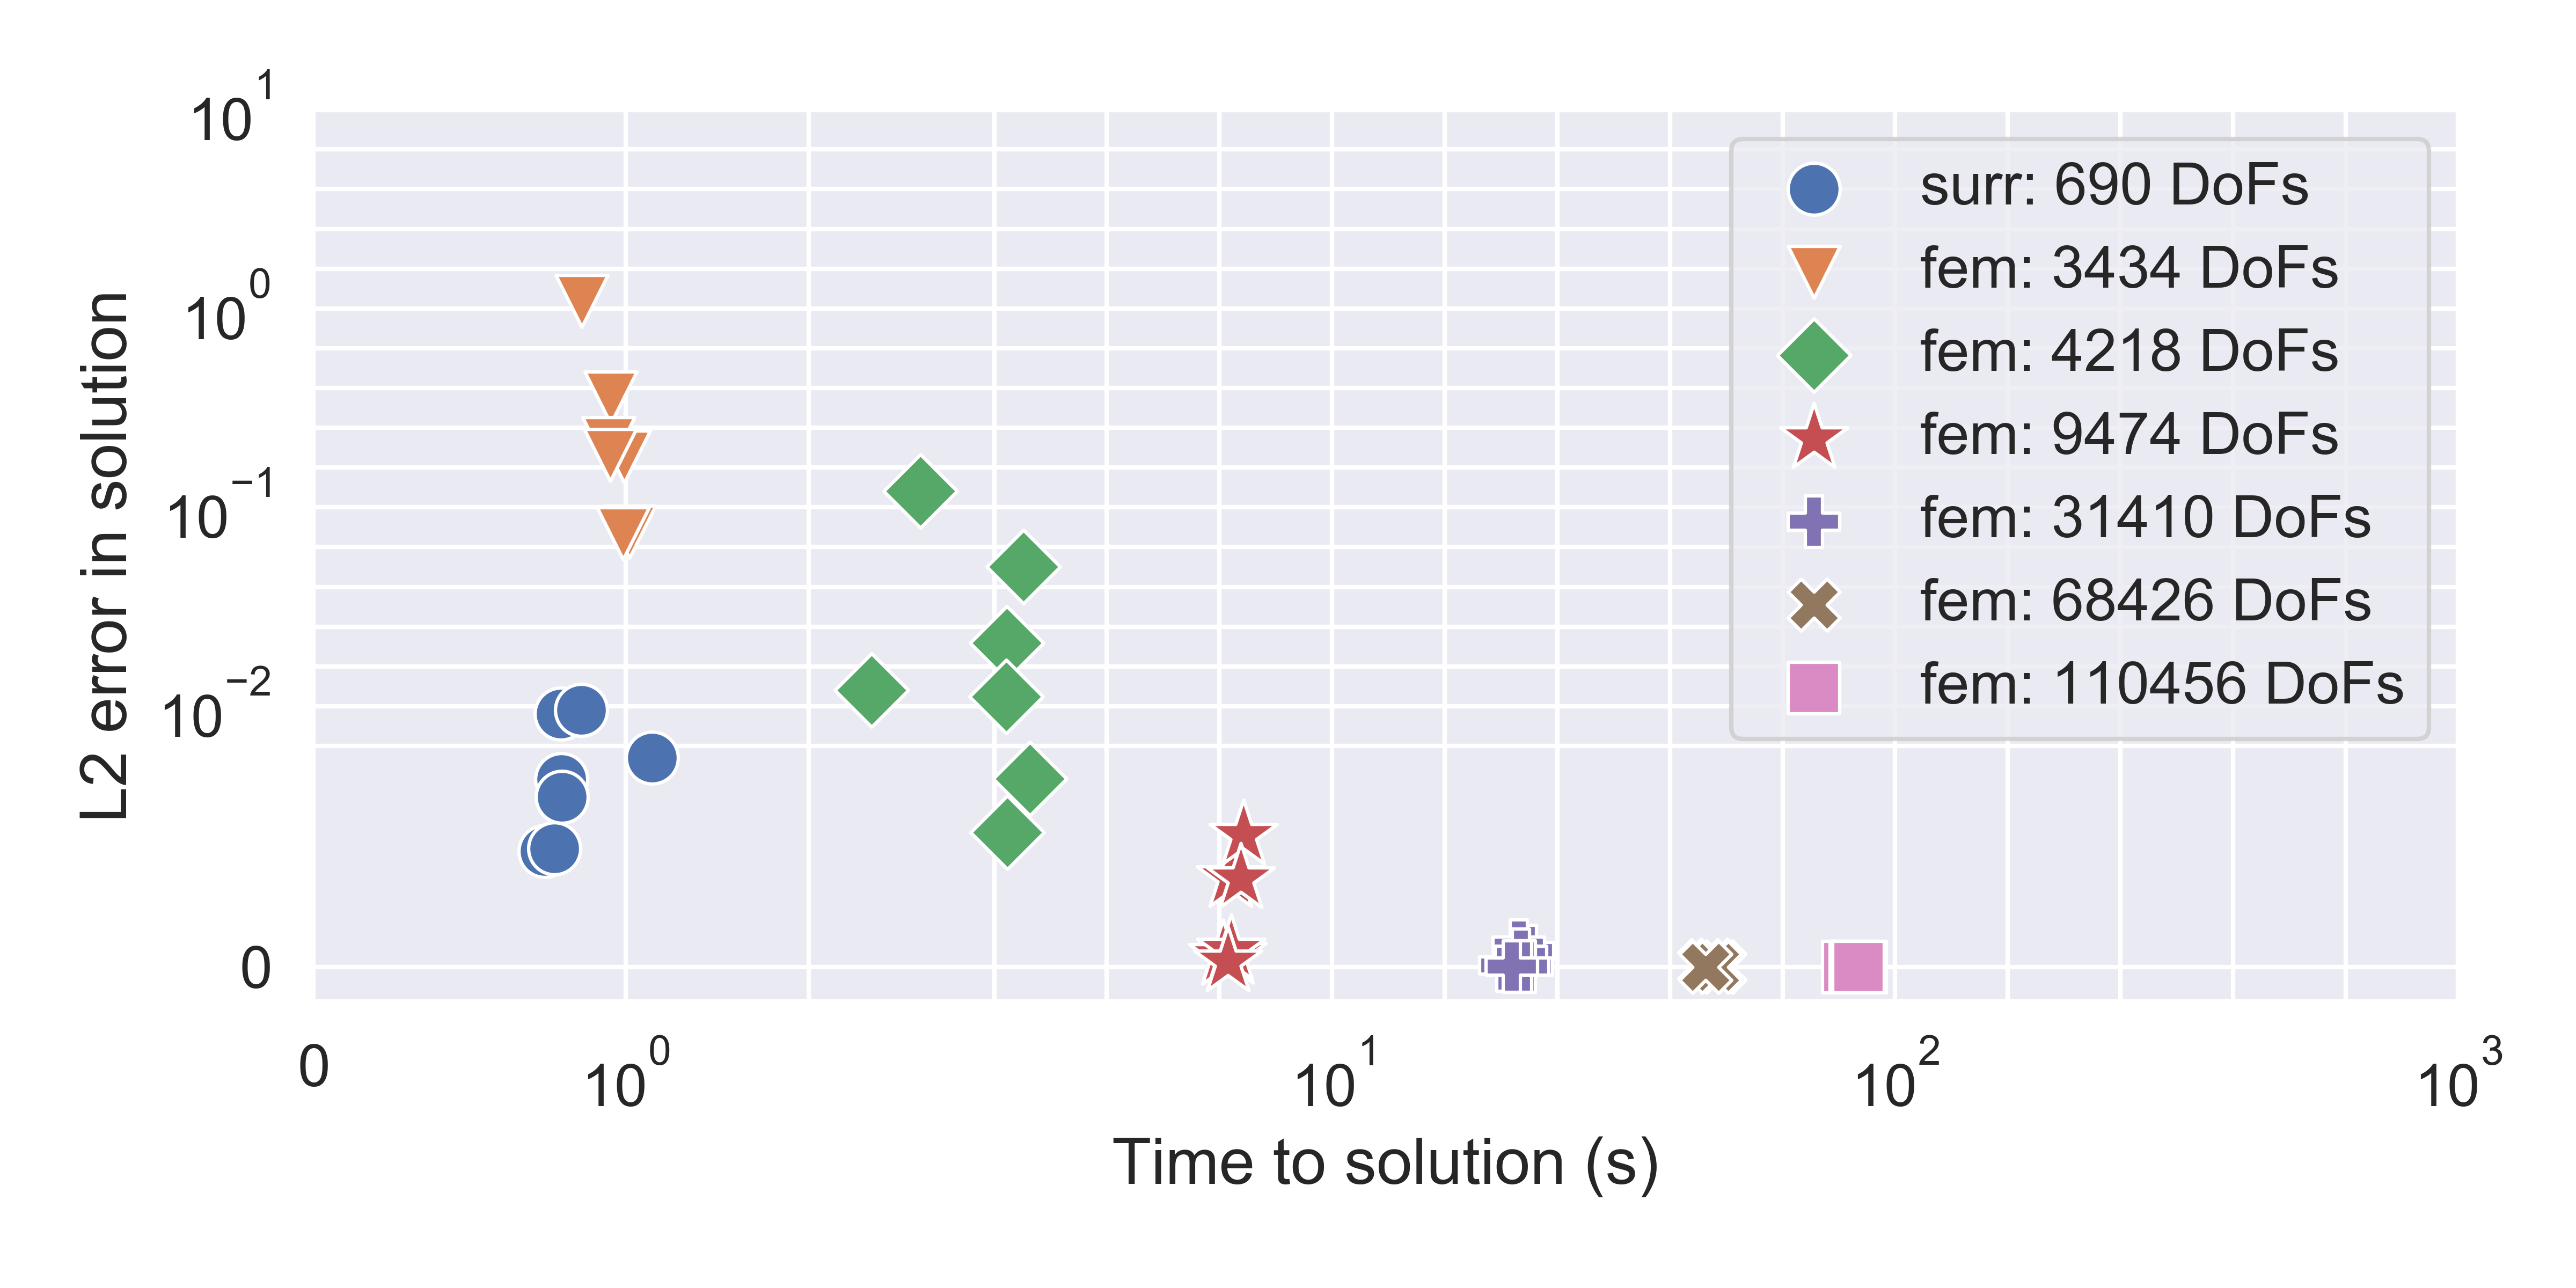
\includegraphics{lces/figures/tension_err.png}
	 \end{adjustbox}
	}}
\end{tabular}
	\vspace{-0.5cm}%
	\caption{\small Error in solution and in estimated energy vs solution wall clock time for the composed energy surrogate and for finite element models with varying mesh sizes. Top: axial compression. Bottom: axial tension.}%
	\label{fig:results}%
 \vspace{-0.3cm}
\end{figure*}

We use PyTorch's L-BFGS routine to minimize the composed surrogate energy, with step size $0.25$ and default criteria for checking convergence. We attempt to solve each finite element model with FEniCS' Newton method with $[1, 2, 5, 10, 20]$ load steps and relaxation parameters $[0.9, 0.7, 0.4, 0.1, 0.05]$, and record time taken for the \emph{fastest} convergent solve.
% We also tried the quasi-Newton method of PETSc \citep{petsc-web-page}, which often did not converge.
Under compression these solids exhibit nonlinear behavior, and only more conservative solves converge. Under tension they behave closer to a linear elastic model, and Newton's method converges quickly. Measurements are taken on an AWS M4.xlarge EC2 CPU instance. Using a GPU could provide further acceleration.
\begin{wrapfigure}[14]{r}{0.34\textwidth}
 \begin{tabular}{c|c}
	 {\resizebox{0.40\linewidth}{!}{
 \begin{adjustbox}{clip, trim=3.35cm 1.7cm 2.7cm 1.8cm}
	 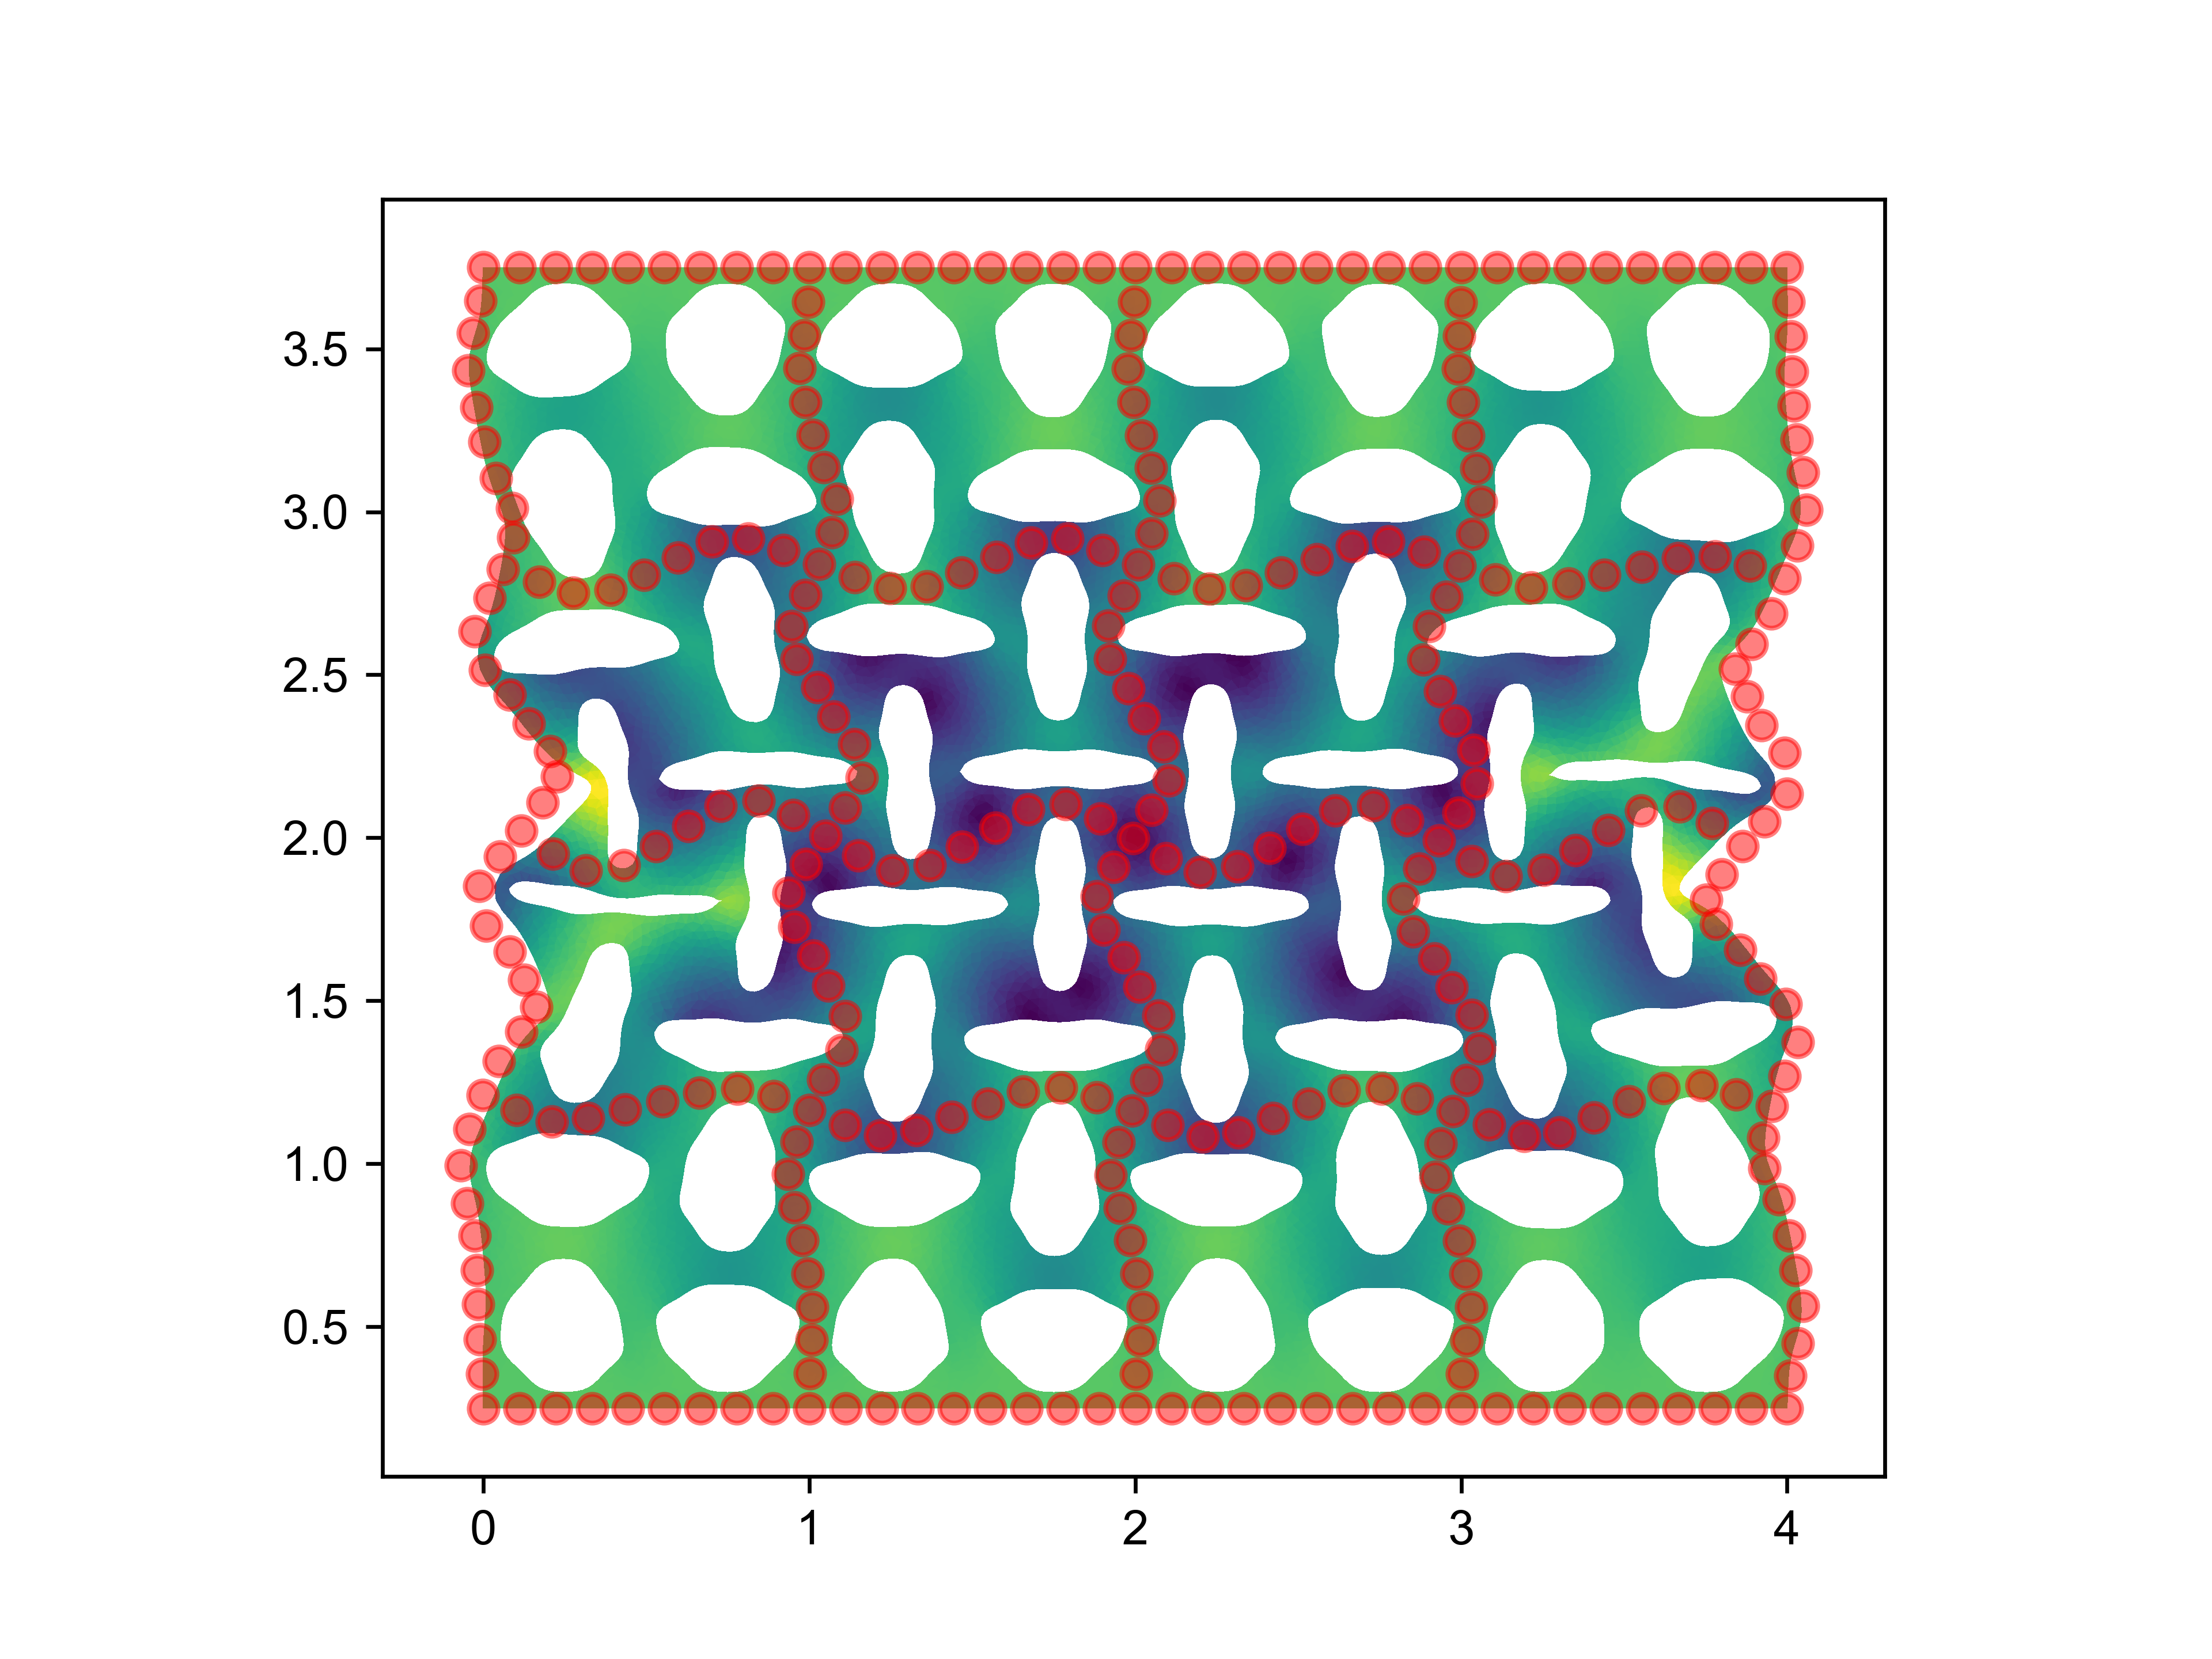
\includegraphics{lces/figures/compress_1.png}
	 \end{adjustbox}
	 }}&
	{\resizebox{0.45\linewidth}{!}{
 \begin{adjustbox}{clip, trim=2.2cm 1.7cm 2.3cm 1.8cm}
	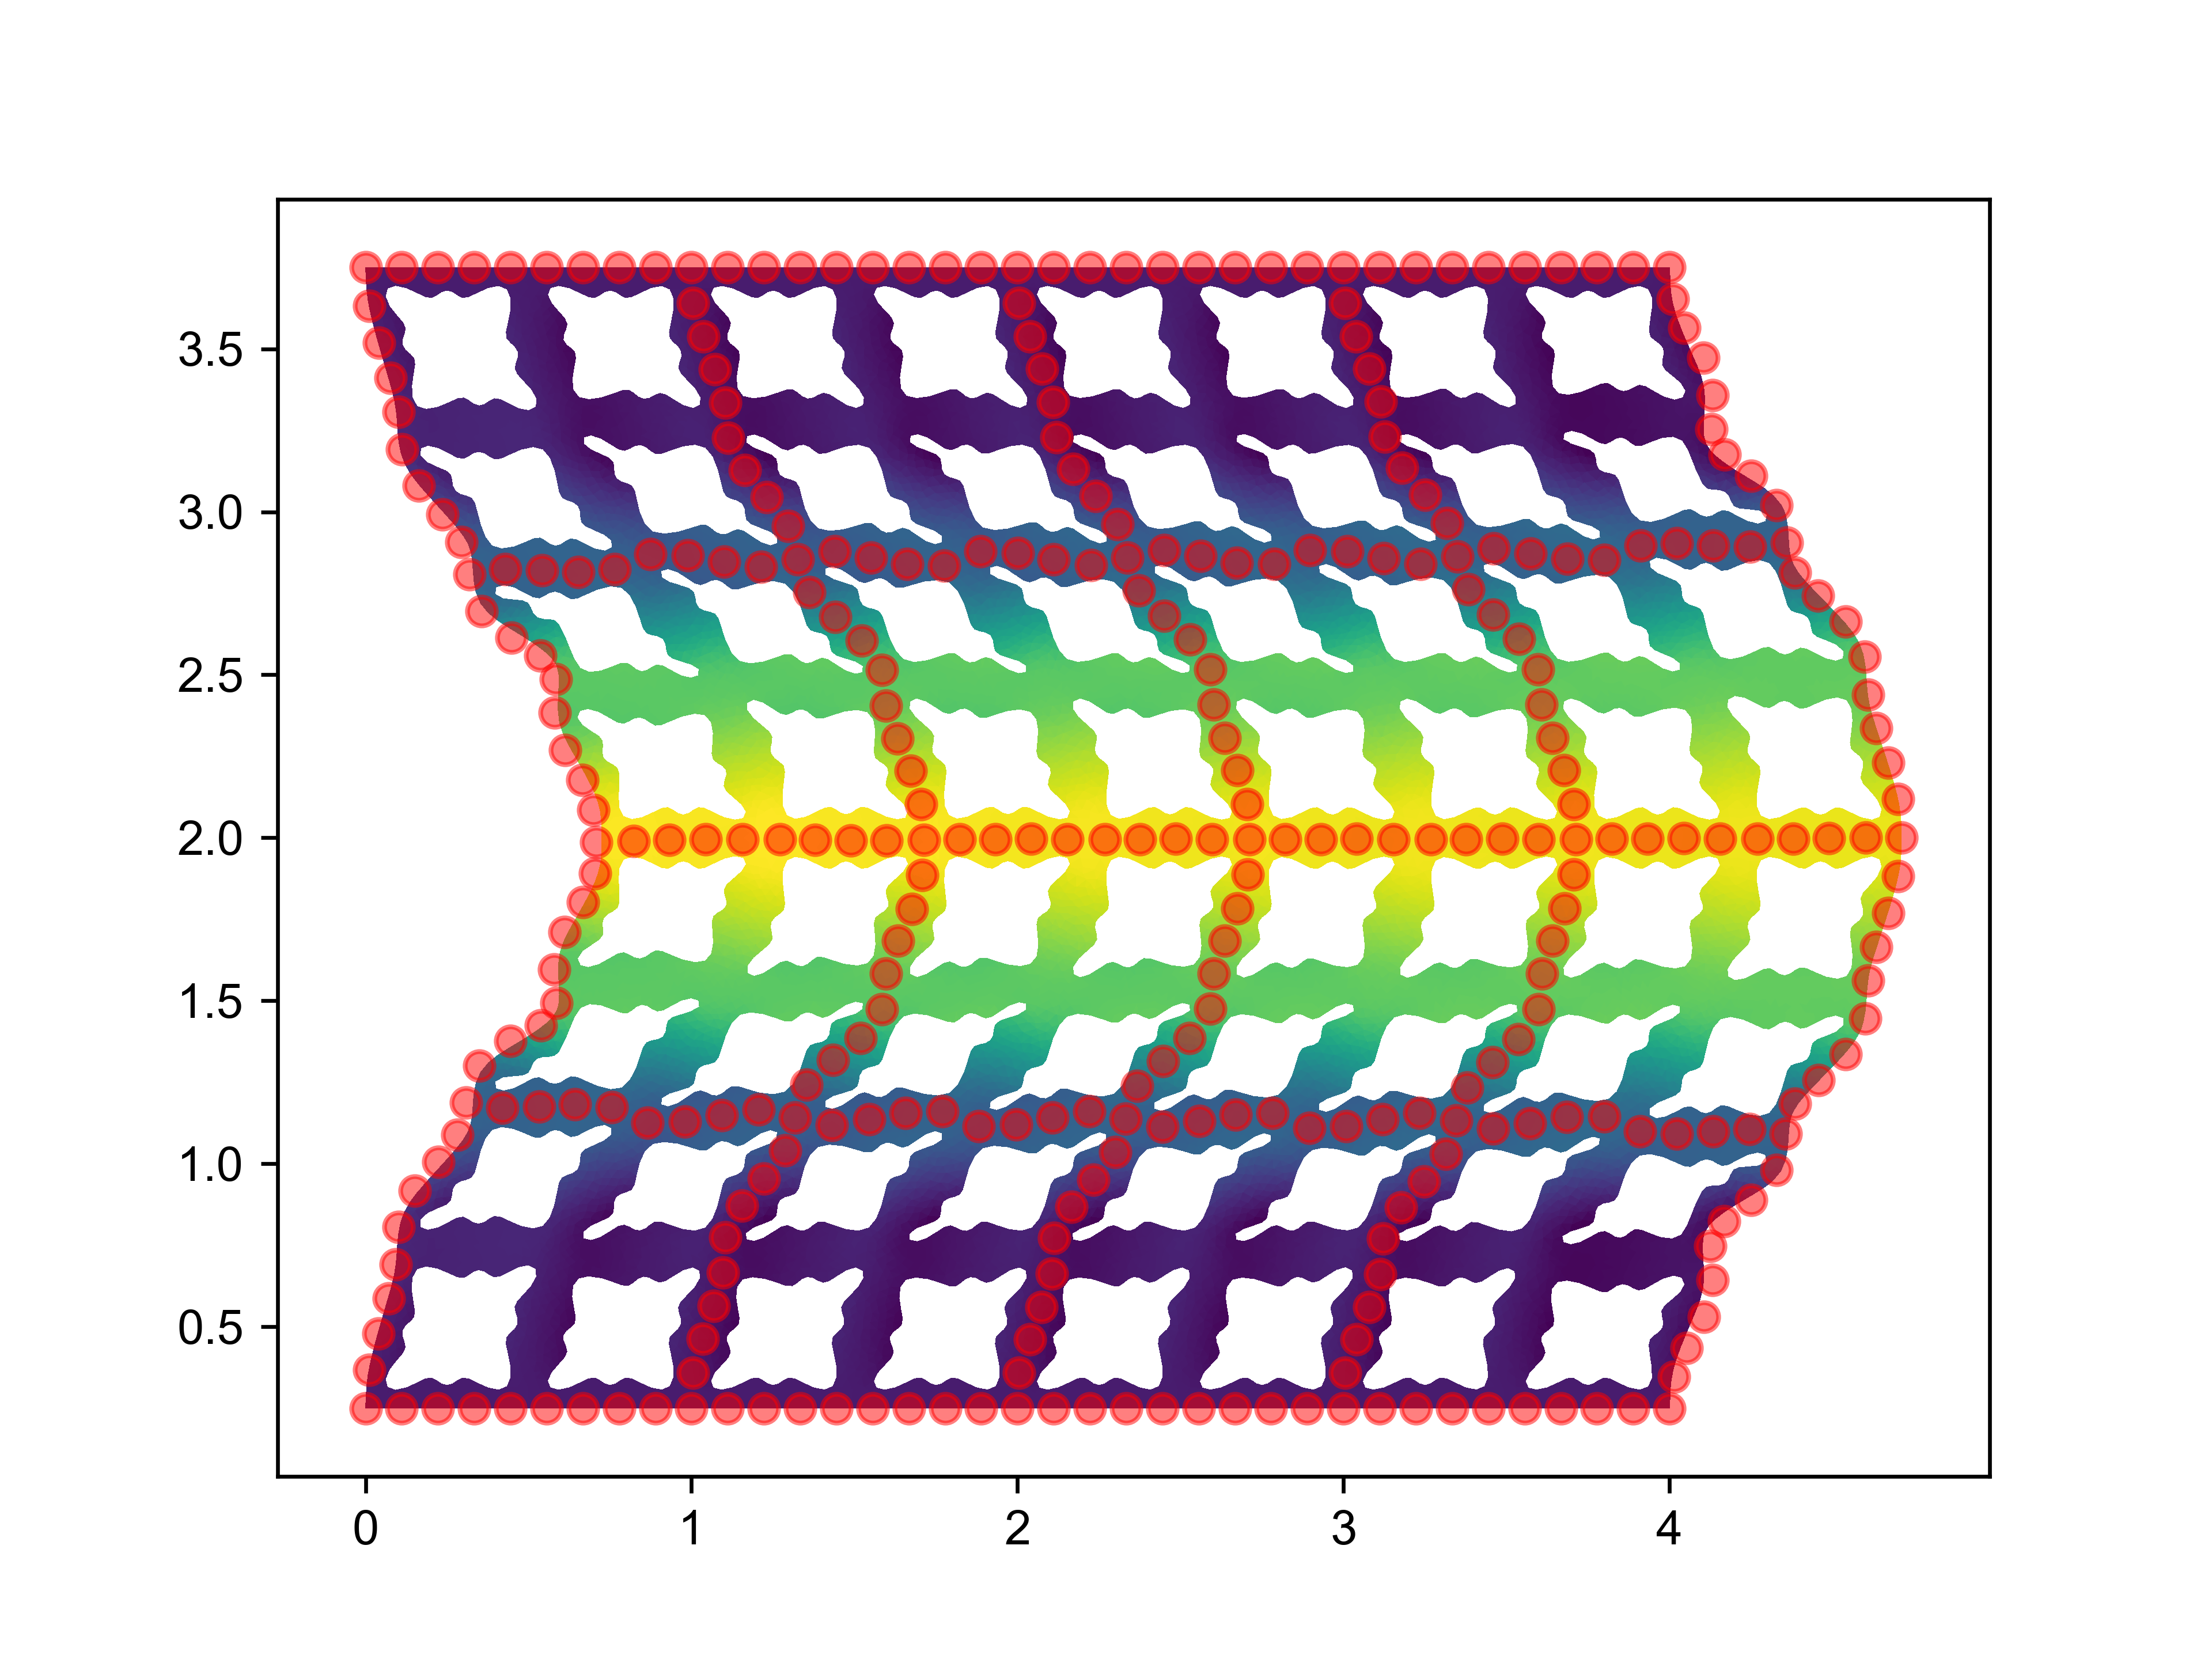
\includegraphics{lces/figures/compress_2.png}
	 \end{adjustbox}
	}}\\\hline
		\rule{0pt}{13ex}
	 {\resizebox{0.33\linewidth}{!}{
 \begin{adjustbox}{clip, trim=4.5cm 1.5cm 4.0cm 1.5cm}
	 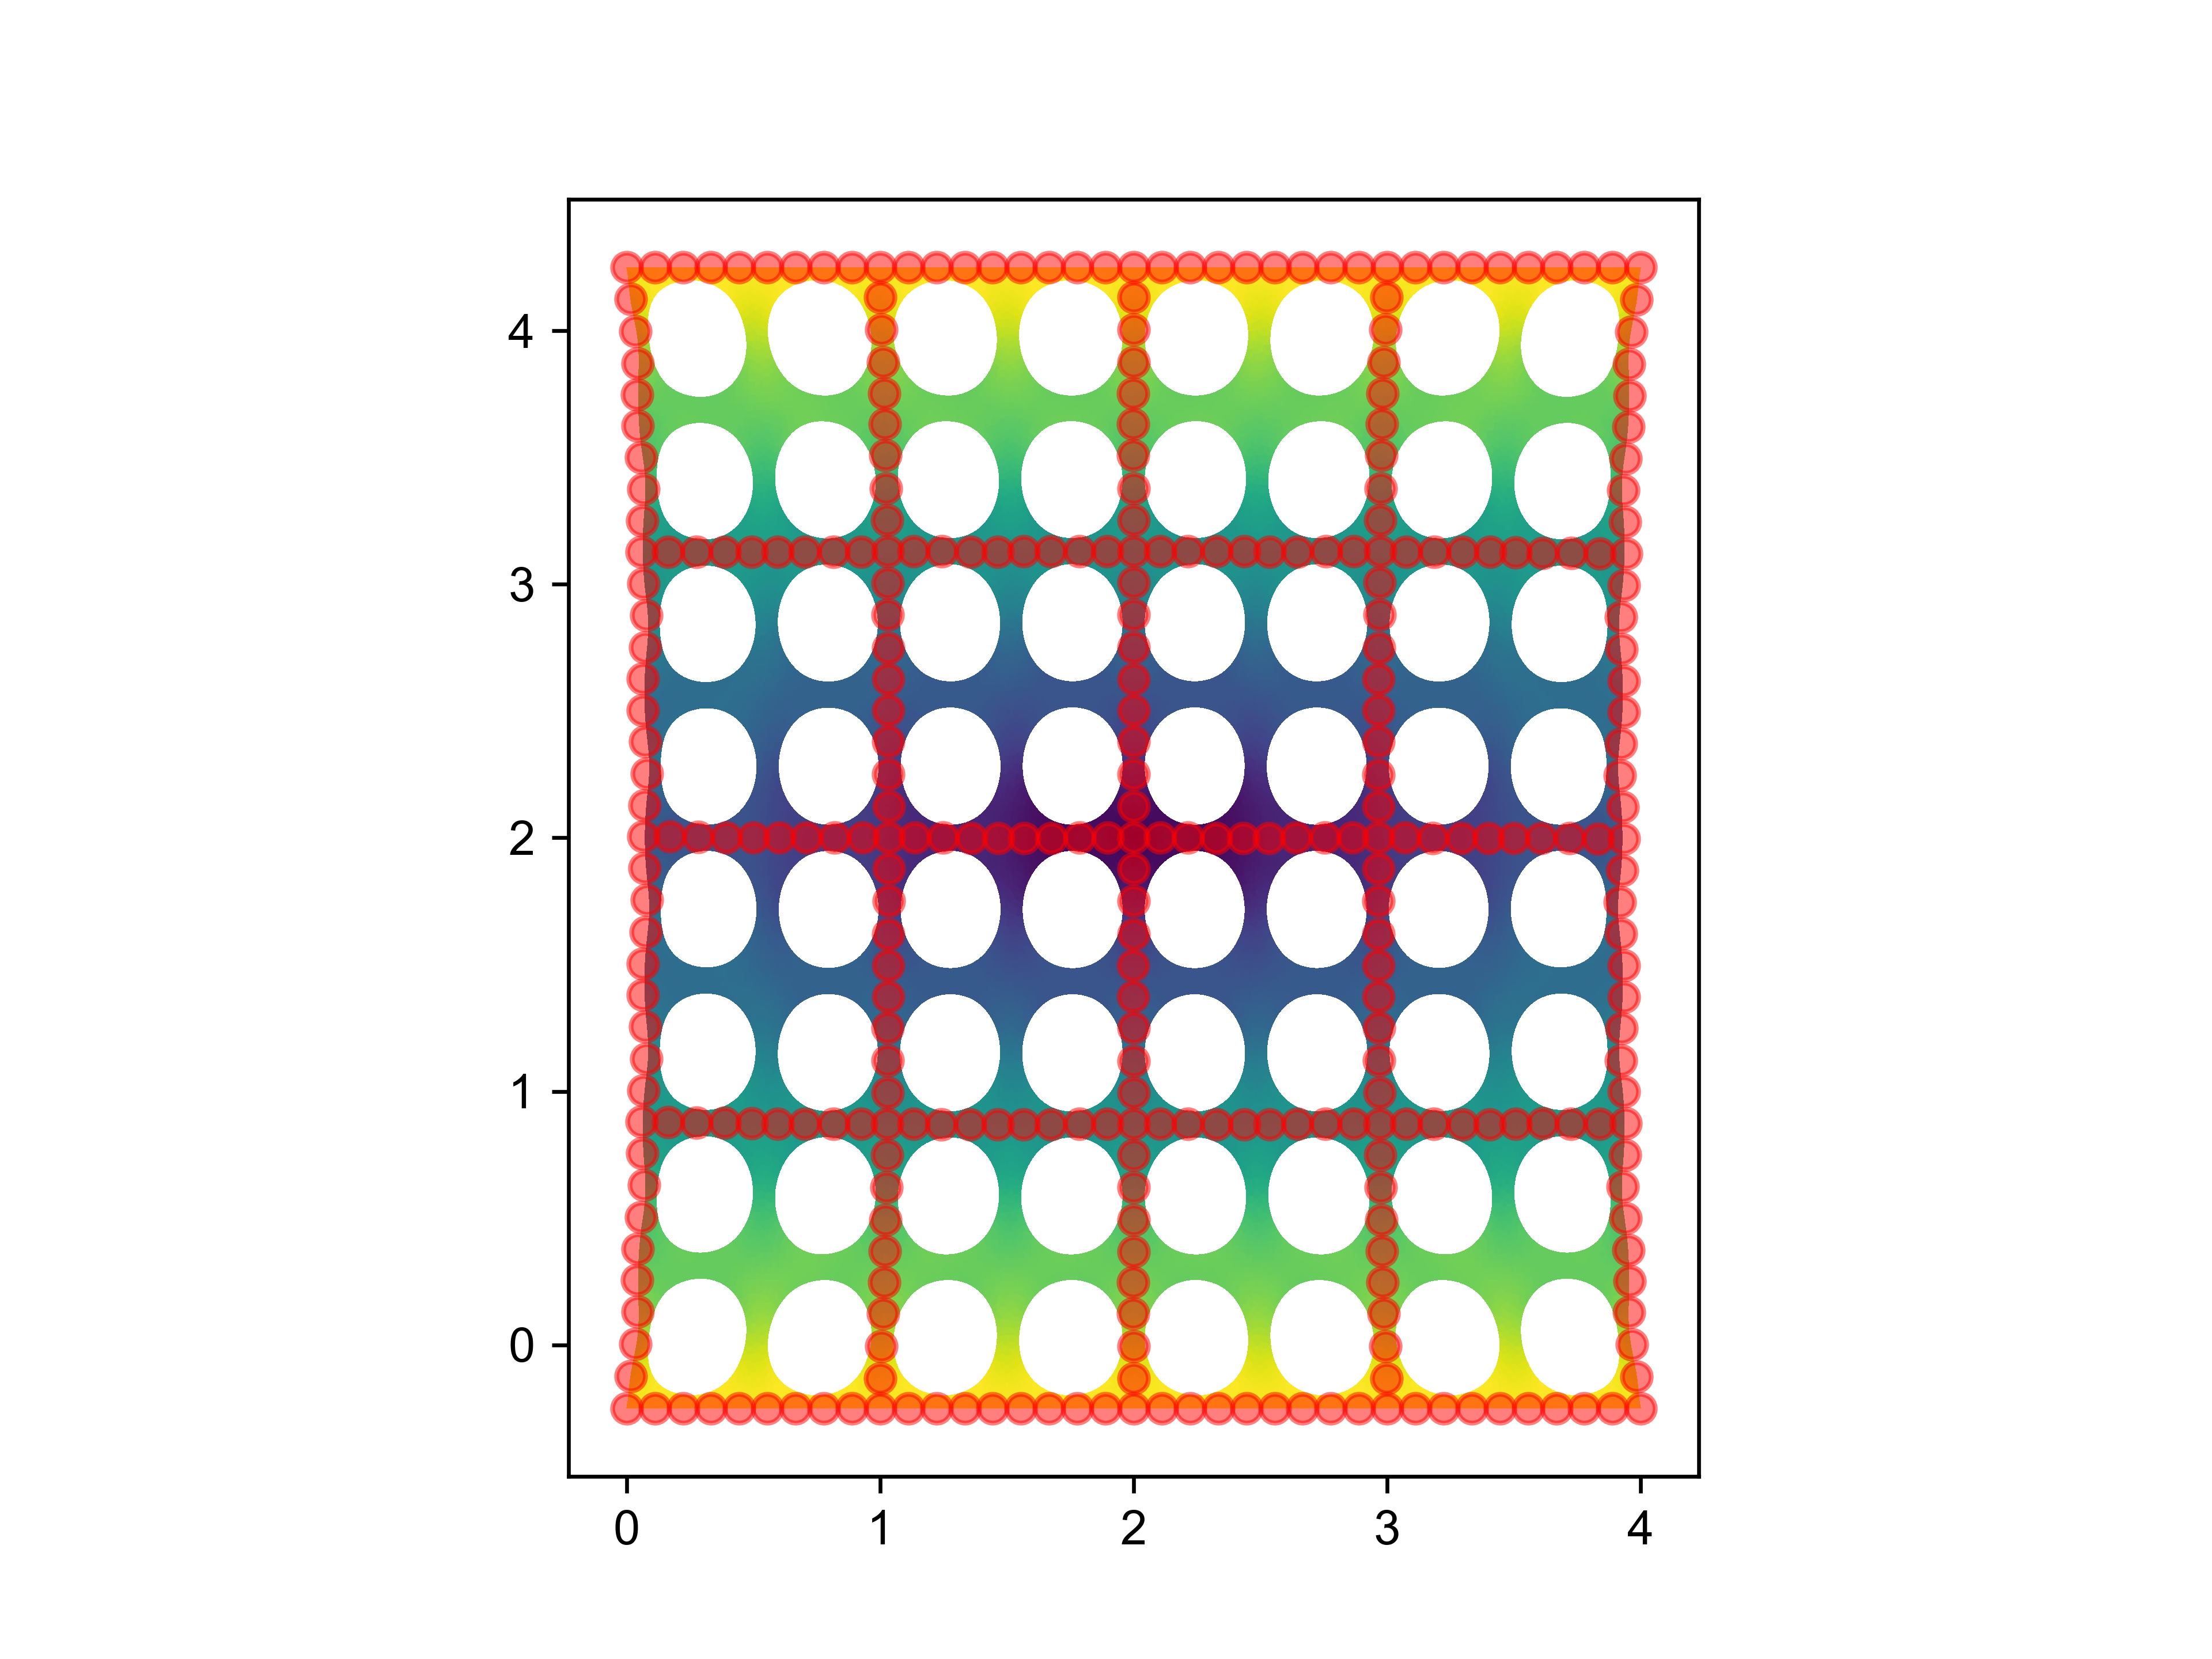
\includegraphics{lces/figures/tension_2.png}
	 \end{adjustbox}
	 }}&
	{\resizebox{0.33\linewidth}{!}{
 \begin{adjustbox}{clip, trim=4.5cm 1.5cm 4.0cm 1.5cm}
	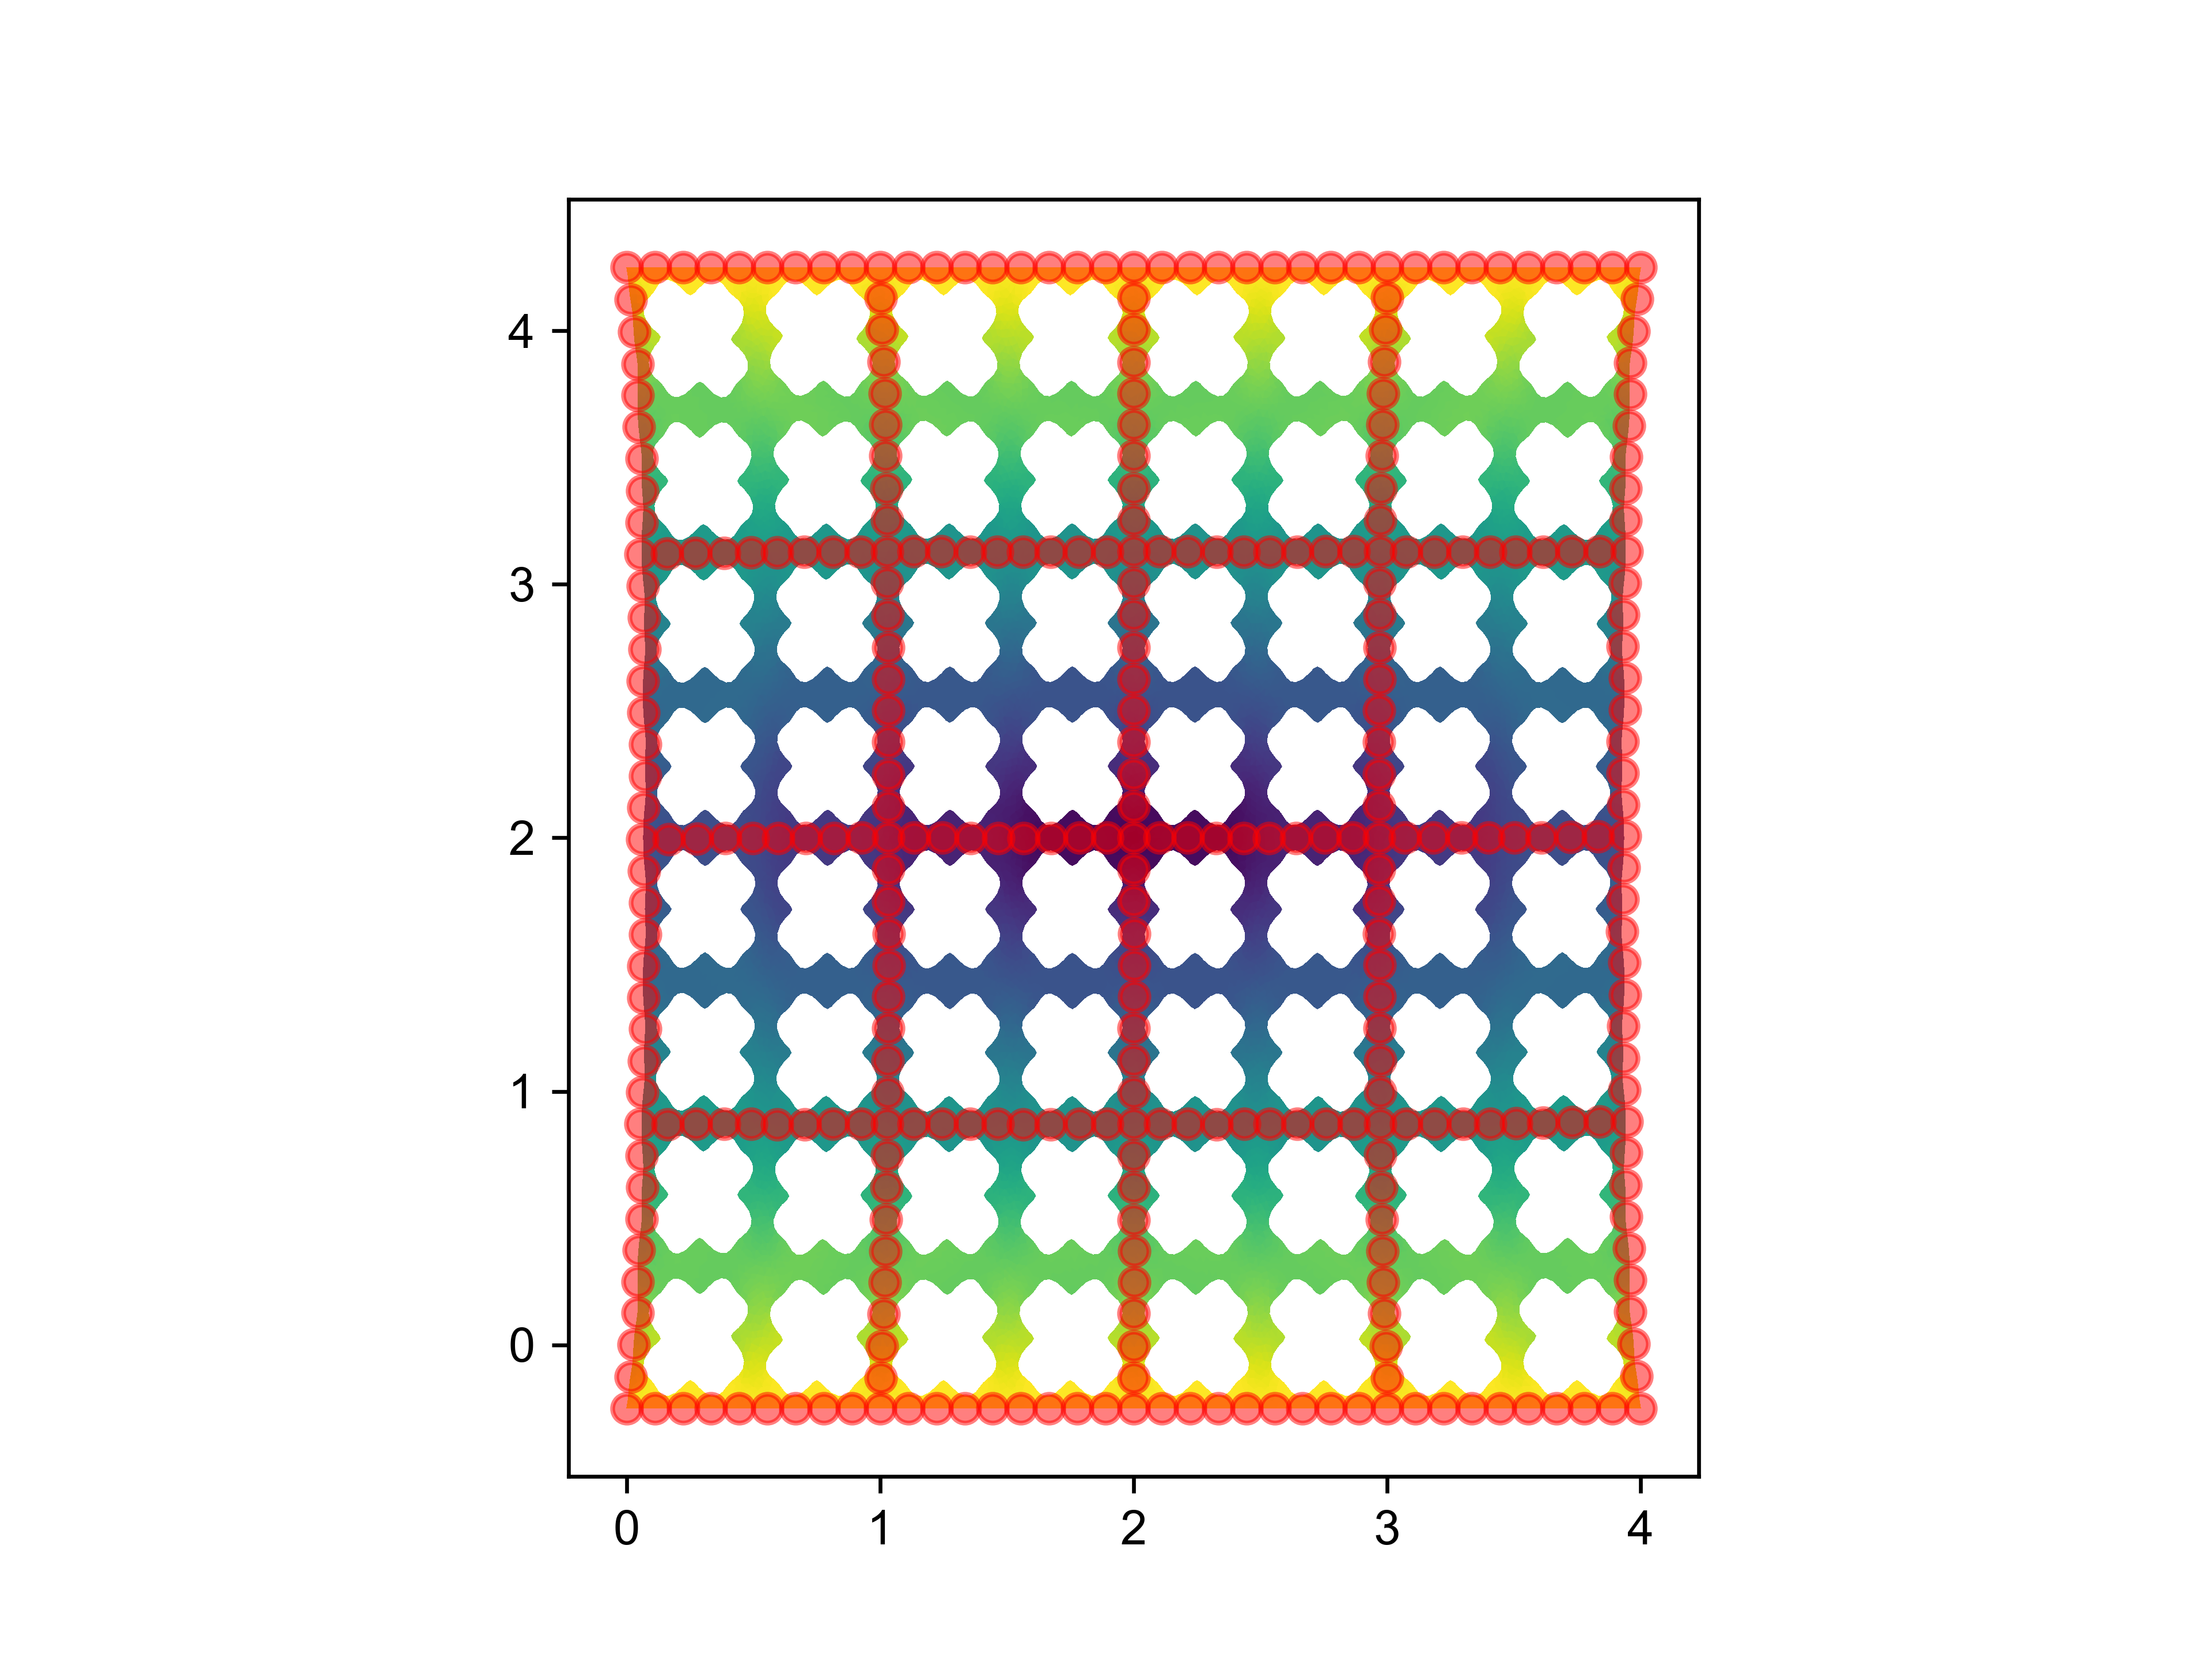
\includegraphics{lces/figures/tension_1.png}
	 \end{adjustbox}
	}}
\end{tabular}
\vspace{-0.3cm}
\caption{\small Meta-materials under compression (top) and tension (bottom), with solution found via CES shown in red at spline control points.}
\vspace{-0.8cm}
\label{fig:compress}
\end{wrapfigure}

We measure error in the solution and in the macroscopic energy. The former is~${||\hat{u}-u^*||_2^2}$, where $\hat{u}$ and $u^*$ are the approximation and ground-truth evaluated at spline control points. The latter is the relative error $\nicefrac{|\hat{E}(\hat{u}) - E^*(u^*)|}{E^*(u^*)}$, where $\hat{E}(\hat{u})$ is the approximated energy of the approximate solution, and $E^*(u^*)$ is the ground-truth energy of the ground-truth solution. As the energy function determines behavior, accuracy of energy is a potential indicator of ability to generalize to larger structures. The highest-fidelity finite element model is taken as ground truth, and thus has an error of zero on both metrics. Multiple minimizers exist as energy is preserved under rigid body transforms, so before comparing a solution~$\hat{u}$ to the ground-truth~$u^*$ we check each vertical and horizontal flip and use the flip which minimizes the solution error.
% \vspace{-0.2cm}

Figure \ref{fig:results} shows our evaluation. Composed energy surrogates are more efficient than high-fidelity FEA simulations yet more accurate than low-fidelity simulations. CES produces solutions with equivalent~$\ell^2$ error to FEA solutions which use an order of magnitude more variables or computation time, and with an order of magnitude less~$\ell^2$ error than FEM solutions requiring the same computation. This gap increases to several orders of magnitude when we consider percentage error in the predicted strain energy. We visualize the ground-truth and the CES approximation in Figure \ref{fig:compress}. See the appendix for visualization of FEM and CES solutions for the remaining structures.

\section{Limitations and opportunities}\label{sec:discussion}
\textbf{Use of \textsc{DAgger}}. We use \textsc{DAgger} to help CES match the ground-truth on the states encountered during the solution trajectory. This requires one to specify in advance the conditions under which the surrogate will be deployed. Investigating CES' ability to generalize to novel deployment conditions--and designing surrogates which can do so effectively--is an important direction for future work.

\textbf{Error estimation, refinement, and guarantees}. Finite element methods permit a straightforward way to estimate the error (compare to the solution in a more-refined basis) and control it (via refinement). CES currently lacks these properties.

\textbf{Finite element baseline}. There is an immense body of work on finite element methods and iterative solvers. We provide a representative baseline, but our work should not be taken as a comparison with the ``state-of-the-art''. We show that composable machine-learned energy surrogates enjoy advantages over a reasonable baseline, and hold promise for scalable amortization of solving modular PDEs.

\textbf{Hyperparameters}. Both our method and the finite element baseline rely on a multitude of hyperparameters: the size of the spline reduced basis; the size and learning rate of the neural network; the size and degree of the finite element approximation; and the specific variant of Newton's method to solve the finite element model. We do not attempt a formal, exhaustive search over these parameters.

\textbf{Known structure}. We leave much fruit on the vine in terms of engineering structure known from the  into our surrogate. For example, one could also use a more expressive normalizer than $||\rvu||_2^2$, e.g. the energy predicted by a coarse-grained linear elastic model, or exploit spatially local correlation, e.g. by using a 1-d convolutional network around the boundary of the cell.
\vspace{-0.2cm}

\section{Conclusion}
We present a framework for collapsing optimization problems with local bilevel structure by learning composable energy surrogates. This framework is applied to amortizing the solution of PDEs corresponding to mechanical meta-material behavior. Learned composable energy surrogates are more efficient than high-fidelity FEA yet more accurate than low-fidelity FEA, occupying a new point on the Pareto frontier. We believe that these surrogates could accelerate meta-material design, as well as design and identification of other systems described by PDEs with parametric modular structure.

\chapter{Efficient optimization of loops and limits with randomized telescoping sums}
We consider optimization problems in which the objective requires an inner loop with many steps or is the limit of a sequence of increasingly costly approximations.
Meta-learning, training recurrent neural networks, and optimization of the solutions to differential equations are all examples of optimization problems with this character.
In such problems, it can be expensive to compute the objective function value and its gradient, but truncating the loop or using less accurate approximations can induce biases that damage the overall solution.
We propose \emph{randomized telescope} (RT) gradient estimators, which represent the objective as the sum of a telescoping series and sample linear combinations of terms to provide cheap unbiased gradient estimates.
We identify conditions under which RT estimators achieve optimization convergence rates independent of the length of the loop or the required accuracy of the approximation.
We also derive a method for tuning RT estimators online to maximize a lower bound on the expected decrease in loss per unit of computation.
We evaluate our adaptive RT estimators on a range of applications including meta-optimization of learning rates, variational inference of ODE parameters, and training an LSTM to model long sequences.


\section{Introduction}
Many important optimization problems consist of objective functions that can only be computed iteratively or as the limit of an approximation.
Machine learning and scientific computing provide many important examples.
In meta-learning, evaluation of the objective typically requires the training of a model, a case of bi-level optimization.
When training a model on sequential data or to make decisions over time, each learning step requires looping over time steps.
More broadly, in many scientific and engineering applications one wishes to optimize an objective that is defined as the limit of a sequence of approximations with both fidelity and computational cost increasing according to a natural number~${n\geq 1}$.
Inner-loop examples include: integration by Monte Carlo or quadrature with~$n$ evaluation points; solving ordinary differential equations (ODEs) with an Euler or Runge Kutta method with~$n$ steps and~$\mathcal{O}(\frac{1}{n})$ step size;
and solving partial differential equations (PDEs) with a finite element basis with size or order increasing with~$n$.

Whether the task is fitting parameters to data, identifying the parameters of a natural system, or optimizing the design of a mechanical part, in this work we seek to more rapidly solve problems in which the objective function demands a tradeoff between computational cost and accuracy.
We formalize this by considering parameters~$\theta\in\mathbb{R}^D$ and a loss function~$\mathcal{L}(\theta)$ that is the uniform limit of a sequence~$\mathcal{L}_n(\theta)$:
\begin{align}
\min_\theta \mathcal{L}(\theta) &= \min_\theta\lim_{n\to\infty}\mathcal{L}_n(\theta)\,.
\label{eqn:opt-problem}
\end{align}
In some problems there may be a finite~${n=H}$ (horizon) that achieves the limit.
We also introduce a cost function~${C:\mathbb{N}_{+}\to\mathbb{R}}$ that is nondecreasing in~$n$ to represent the cost of computing $\mathcal{L}_n$ and its gradient.

A principal challenge of optimization problems with the form in Eq.\ref{eqn:opt-problem} is selecting a finite~$N$ such that the minimum of the surrogate~$\mathcal{L}_N$ is close to that of~$\mathcal{L}$, but without~$\mathcal{L}_N$ (or its gradients) being too expensive.
Choosing a large $N$ can be computationally prohibitive, while choosing a small $N$ may bias optimization.
Meta-optimizing learning rates with truncated horizons can choose wrong hyperparameters by orders of magnitude \cite{wu2018understanding}.
Truncating backpropogation through time for recurrent neural networks (RNNs) favors short term dependencies \cite{tallec2017unbiasing}.
Using too coarse a discretization to solve an ODE or PDE can cause error in the solution and bias outer-loop optimization.
These optimization problems thus experience a sharp trade off between efficient computation and bias.

We propose \emph{randomized telescope} (RT) gradient estimators, which provide cheap unbiased gradient estimates to allow efficient optimization of these objectives.
RT estimators represent the objective or its gradients as a telescoping series of differences between intermediate values, and draw weighted samples from this series to maintain unbiasedness while balancing variance and expected computation.

The paper proceeds as follows.
Section 2 introduces RT estimators and their history.
Section 3 formalizes using RT estimators for optimization, and discusses related work in optimization.
Section 4 proves RT estimators can achieve optimization guarantees for loops and limits.
Section 5 discusses designing RT estimators by maximizing a bound on expected improvement per unit of computation.
Section 6 describes practical considerations adapting RT estimators online.
Section 7 presents experimental results.
Section 8 discusses limitations and future work.
Appendix A presents algorithm pseudocode.
Appendix B presents proofs.

% save some of these refs to add back in
%An important subclass of such objectives is the output of programs with an
%inner loop. Here,
%$X_n$ is some output after unrolling the loop for $n$
%(or a monotonic function of $n$) steps.
%Examples include recurrent and sequence models,
%learning algorithms and meta-learners,
%the deployment of policies in an RL environment,
%models which include repeated application of an operator as part of
%their forward pass such as hypernetwork-CNNs \cite{ha2016hypernetworks}
%or neural ODEs \cite{chen2018neural},
%iterative solution of optimization problems,
%and iterative methods
%for solving systems of equations.

\section{Unbiased randomized truncation}
In this section, we discuss the general problem of estimating limits through randomized truncation.
The first subsection presents the randomized telescope family of unbiased estimators, while the second subsection describes their history (dating back to von Neumann and Ulam).
In the following sections, we will describe how this technique can be used to provide cheap unbiased gradient estimates and accelerate optimization for many problems.

\subsection{Randomized telescope estimators}
Consider estimating any quantity~${Y_H := \lim_{n \to H} Y_n}$ for~${n\in\mathbb{N}_{+}}$ where~${H\in\mathbb{N}_{+}\cup\{\infty\}}$.
Assume that we can compute $Y_n$ for any finite~${n\in\mathbb{N}_{+}}$, but since the cost is nondecreasing in~$n$ there is a point at which this becomes impractical.
Rather than truncating at some fixed value short of the limit, then, we may find it useful to construct an unbiased estimator of~$Y_H$ and take on some randomness in return for reduced computational cost.

Define the backward difference~$\Delta_n$ and represent the quantity of interest $Y_H$ with a telescoping series:
\begin{align*}
Y_H &= \sum_{n=1}^H \Delta_n & \text{where}\quad    \Delta_n &= \begin{cases}
    Y_n - Y_{n-1} & n > 1\\
    Y_1 & n = 1
    \end{cases}\,.
\end{align*}
We may sample from this telescoping series to provide unbiased estimates of~$Y_H$, introducing variance to our estimator in exchange for reducing expected computation.
We use the name \emph{randomized telescope} (RT) to refer to the family of estimators indexed by a distribution~$q$ over the integers~${1,\ldots,H}$ and a weight function $W(n, N)$:
\begin{align}\label{eq:rt_general}
\hat{Y}_H = \sum_{n=1}^N \Delta_n W(n, N) \quad \quad  N \in \{1,\ldots,H\} \sim q\,.
\end{align}

\begin{proposition}\label{prop:unbiased}
\textbf{Unbiasedness of RT estimators.}
The RT estimators in (\ref{eq:rt_general}) are unbiased estimators of
$Y_H$ as long as
\begin{align}
\mathbb{E}_{N\sim q} [W(n, N)] = \sum_{N=n}^H W(n, N)q(N) = 1 \quad \forall n\,.
\end{align}
\end{proposition}
%
See Appendix B for a short proof.
Although we are coining the term ``randomized telescope'' to refer to the family of estimators with the form of Eq.~\ref{eq:rt_general}, the underlying trick has a long history, discussed in the next section.
The literature we are aware of focusses on one or both of two special cases of Eq.~\ref{eq:rt_general}, defined by choice of weight function $W(n, N)$.
We will also focus on these two variants of RT estimators, but we observe that there is a larger family.

Most related work uses the ``Russian roulette'' estimator originally discovered and named by von Neumann and Ulam \cite{kahn1955use}, which we term \emph{RT-RR} and has the form
\begin{align}
W(n, N) = \frac{1}{1 - \sum_{n'=1}^{n-1}q(n')} \mathbbm{1}\{N \geq n\}\,.
\end{align}
It can be seen as unrolling and summing the iterates~$\Delta_n$ while flipping a biased coin at each new iterate $\Delta_n$.
With probability~$q(n)$, the series is truncated at term~$n$ and the unrolling stops.
With probability~${1 - q(n)}$, the process continues, and all future terms are upweighted by $\frac{1}{1-q(n)}$ to maintain unbiasedness.

The other important special case of Eq.~\ref{eq:rt_general} is the ``single sample'' estimator \emph{RT-SS}, referred to as ``single term weighted truncation'' in \citet{lyne2015russian}.
RT-SS takes
\begin{align}
W(n, N) &= \frac{1}{q(N)} \mathbbm{1} \{n = N\}\,.
\end{align}
This is directly importance sampling the differences~$\Delta_n$.

We will later prove conditions under which RT-SS and RT-RR should be preferred.
Of all estimators in the form of (\ref{eq:rt_general}) which obey proposition \ref{prop:unbiased} and for all $q$, RT-SS minimizes the worst-case variance across an adversarial choice of diagonal covariances $\Cov(\Delta_i, \Delta_j)$.
Within the same family, RT-RR achieves minimum variance when $\Delta_i$ and $\Delta_j$ are independent for all $i, j$.

\subsection{A brief history of unbiased randomized truncation}
\label{sec:history}
The essential trick---unbiased estimation of a quantity via randomized truncation of a series---dates back to unpublished work from John von Neumann and Stanislaw Ulam.
They are credited for using it to develop a Monte Carlo method for matrix inversion in \citet{forsythe1950matrix}, and for a method for particle diffusion in \citet{kahn1955use}.

It has been applied and rediscovered in a number of fields and applications.
The early work from von Neumann and Ulam led to its use in computational physics, in neutron transport problems \citep{spanier1969monte}, for studying lattice fermions \citep{kuti1982stochastic}, and to estimate functional integrals \citep{wagner1987unbiased}.
In computer graphics \citet{arvo1990particle} introduced its use for ray tracing; it is now widely used in rendering software.
In statistical estimation, it has been used for estimation of derivatives \citep{rychlik1990unbiased}, unbiased kernel density estimation \citep{rychlik1995class}, doubly-intractable Bayesian posterior distributions \citep{girolami2013playing, lyne2015russian, wei2016markov}, and unbiased MCMC \citep{jacob2017unbiased}.

The underlying trick has been rediscovered by \citet{fearnhead2008particle} for unbiased estimation in particle filtering, by \citet{mcleish2010general} for debiasing Monte Carlo estimates, by \citet{rhee2012new, rhee2015unbiased} for unbiased estimation in stochastic differential equations,
and by \citet{tallec2017unbiasing} to debias truncated backpropagation.
The latter also uses RT estimators for optimization; however, it only considers fixed ``Russian roulette''-style randomized telescope estimators and does not consider convergence rates or how to adapt the estimator online (our main contributions).

\section{Optimizing loops and limits}
In this paper, we consider optimizing functions defined as limits, where loops are an important special case.
Consider a problem where, given parameters~$\theta$ we can obtain a series of approximate losses $\mathcal{L}_n(\theta)$, which converges uniformly to some limit ${\lim_{n \to H} \mathcal{L}_n := \mathcal{L}}$, for ~${n\in\mathbb{N}_{+}}$ and~${H\in\mathbb{N}_{+}\cup\{\infty\}}$.
We assume the sequence of gradients with respect to~$\theta$, denoted ${G_n(\theta) := \nabla_\theta\mathcal{L}_n(\theta)}$ converge uniformly to a limit ~${G(\theta)}$.
Under this uniform convergence and assuming convergence of $\mathcal{L}_n$, we have ~${\lim_{n \to H} \nabla_{\theta}\mathcal{L}_n(\theta) = \nabla_{\theta}\lim_{n \to H}\mathcal{L}_n(\theta)}$ (see Theorem 7.17 in \citet{rudin1976principles}), and so ~${G(\theta)}$ is indeed the gradient of our objective ~${\mathcal{L}(\theta)}$.
We assume there is some computation cost $C(n)$ associated with evaluating~$\mathcal{L}_n$ or $G_n$, which is nondecreasing with $n$, and we wish to efficiently minimize $\mathcal{L}$ with respect to~$\theta$.
Loops are a special case of this framework, where $\mathcal{L}_n$ is the loss resulting from running the loop for some number of steps increasing in $n$.

\subsection{Randomized telescopes for optimization}
We propose using randomized telescopes to provide a stochastic gradient estimator for such optimization problems.
Our aim is to accelerate optimization in much the same manner as minibatch stochastic gradient descent accelerates optimization for large datasets: using sampling to decrease the expected computation cost of each optimization step, at the price of increasing variance in the gradient estimates, without introducing bias.

Consider the gradient~${G(\theta) = \lim_{n \to H} G_n(\theta)}$, and the backward difference ${\Delta_n(\theta) = G_n(\theta) - G_{n-1}(\theta)}$, where~${G_0(\theta) = 0}$, so that~${G(\theta) = \sum_{n=1}^H \Delta_n(\theta)}$.
We use the randomized telescope estimator
\begin{align}
\hat{G}(\theta) &= G_N(\theta) = \sum_{n=1}^N\Delta_n(\theta) W(n,N)
\end{align}
where ${N \in \{1,2,\ldots,H\}}$ is drawn according to a proposal distribution~$q$, and together~$W$ and~$q$ satisfy proposition~\ref{prop:unbiased}.

Note that due to linearity of differentiation, and letting ${\mathcal{L}_0(\theta) := 0}$, we have
\begin{align*}
\sum_{n=1}^N\! \Delta_n(\theta) W(n, N) =
\nabla_\theta\!\! \sum_{n=1}^N\!
(\mathcal{L}_n(\theta)\! -\! \mathcal{L}_{n-1}(\theta))  W(n, N)\,.
\end{align*}
Thus, when computing $\mathcal{L}_n(\theta)$ can reuse most of the computation performed for computing $\mathcal{L}_{n-1}(\theta)$, we can evaluate~$\hat{G}_N(\theta)$ via forward or backward automatic differentiation with cost approximately equal to computing~$G_N(\theta)$, i.e.,~$\hat{G}_N(\theta)$ has computation cost $\approx C(N)$.
This most often occurs when evaluating $\mathcal{L}_n(\theta)$ involves an inner loop and the step size used for the inner loop does not change with~$n$, such as in meta-learning and training RNNs.
When computing $\mathcal{L}_n(\theta)$ does not reuse computation, e.g., when solving an ODE or PDE where~$n$ describes how fine a discretization to use, evaluating $\hat{G}_N(\theta)$ requires separately computing $\mathcal{L}_n(\theta)$ for all~${n \leq N}$ for which~${W(n, N) \neq 0}$, i.e.,~$\hat{G}_N(\theta)$ has computation cost~${\sum_{n=1}^N C(n) \mathbbm{1} \{W(n, N) \neq 0\}}$.

\subsection{Related work in optimization}
Gradient-based bilevel optimization has seen extensive work in literature.
See \citet{jameson1988aerodynamic} for an early example of optimizing implicit functions, \citet{christianson1998reverse} for a mathematical treatment, and \citet{maclaurin2015gradient, franceschi2017forward} for recent treatments in machine learning.
\citet{shaban2018truncated} propose truncating only the backward pass by only backpropagating through the final few optimization steps to reduce memory requirements.
\citet{metz2018learned} propose linearly increasing the number of inner steps over the course of the outer optimization.

An important case of bi-level optimization is optimization of architectures and hyperparameters.
Truncation causes bias, as shown by \citet{wu2018understanding} for learning rates and by \citet{metz2018learned} for neural optimizers.

Bi-level optimization is also used for meta-learning across related tasks \citep{schmidhuber1987evolutionary, bengio1992optimization}.
\citet{ravi2016optimization} train an initialization and optimizer, and \citet{finn2017model} only an initialization, to minimize validation loss.
The latter paper shows increasing performance with the number of steps used in the inner optimization.
However, in practice the number of inner loop steps must be kept small to allow training over many tasks.

Bi-level optimization can be accelerated by amortization.
Variational inference can be seen as bi-level optimization; variational autoencoders \citep{kingma2013auto} amortize the inner optimization with a predictive model of the solution to the inner objective.
Recent work such as \citet{brock2018smash, lorraine2018stochastic} amortizes hyperparameter optimization in a similar fashion.

However, amortizing the inner loop induces bias.
\citet{cremer2018inference} demonstrate this in VAEs, while \citet{kim2018semi} show that in VAEs, combining amortization with truncation by taking several gradient steps on the output of the encoder can reduce this bias.
This shows these techniques are orthogonal to our contributions: while fully amortizing the inner optimization causes bias, predictive models of the limit can accelerate convergence of $\mathcal{L}_n$ to $\mathcal{L}$.

Our work is also related to work on training sequence models.
\citet{tallec2017unbiasing} use the Russian roulette estimator to debias truncated backpropagation through time.
They use a fixed geometrically decaying~$q(N)$, and show that this improves validation loss for Penn Treebank.
They do not consider efficiency of optimization, or methods to automatically set or adapt the hyperparameters of the randomized telescope.
\citet{trinh2018learning} learn long term dependencies with auxiliary losses.
Other work accelerates optimization of sequence models by replacing recurrent models which require backpropagation through time with models which use convolution or attention \citep{vaswani2017attention}, which can be trained more efficiently.

\section{Convergence rates with fixed RT estimators}
Before considering more complex large-scale problems, we examine the simple RT estimator for stochastic gradient descent on convex problems.
We assume that the sequence ~$\mathcal{L}_n(\theta)$ and units for $C$ are chosen such that~$C(n) = n$.
We study RT-SS, with ~$q(n)$ fixed \emph{a priori}.
We consider optimizing parameters~${\theta \in \mathcal{K}}$, where~${\mathcal{K} \subset \mathcal{R}^d}$ is a bounded, convex and compact set with diameter bounded by $D$.
We assume~$\mathcal{L}(\theta)$ is convex in~$\theta$, and ~$G_n(\theta)$ converge according to~${||\Delta_n||_2 \leq \psi_n}$, where~$\psi_n$ converges polynomially or geometrically.
The quantity of interest is the instantaneous regret,~${R_t = \mathcal{L}(\theta_t) - \min_{\theta} \mathcal{L} (\theta)}$, where~$\theta_t$ is the parameter after~$t$ steps of SGD.

In this setting, any fixed truncation scheme using~$\mathcal{L}_N$ as a surrogate for~$\mathcal{L}$, with fixed ${N < H}$, cannot achieve~${\lim_{t \to \infty} R_t = 0}$.
Meanwhile, the fully unrolled estimator has computation cost which scales with~$H$.
In the many situations where~${H \to \infty}$, it is impossible to take even a single gradient step with this estimator.

The randomized telescope estimator overcomes these drawbacks by exploiting the fact that~$G_n$ converges according to~$||\Delta_n||_2 \leq \psi_n$.
As long as~$q$ is chosen to have tails no lighter than~$\psi_n$, for sufficiently fast convergence, the resulting RT-SS gradient estimator achieves asymptotic regret bounds invariant to~$H$ in terms of convergence rate.

All proofs are deferred to Appendix B.
We begin by proving bounds on the variance and expected computation for polynomially decaying~$q(n)$ and~$\psi_n$.
\begin{theorem}\label{thm:poly}
\textbf{Bounded variance and compute with polynomial convergence of $\psi$}.
Assume~$\psi$ converges according to~$\psi_n \leq \frac{c_\psi}{(n)^p}$ or faster, for constants ${p > 0}$ and~$c_\psi > 0$.
Choose the RT-SS estimator with ${q(n) \propto 1/((n)^{p + 1/2})}$.
The resulting estimator~$\hat{G}$ achieves expected compute~${C \leq (\mathcal{H}_{H}^{p-\frac{1}{2}})^2}$, where~$\mathcal{H}_H^i$ is the~$H$th generalized harmonic number of order~$i$, and expected squared norm $\mathbb{E}[ ||\hat{G}||_2^2 ] \leq c_{\psi}^2 (\mathcal{H}_H^{p-\frac{1}{2}})^2 := \tilde{G}^2$.
The limit~${\lim_{H \to \infty} \mathcal{H}_H^{p - \frac{1}{2}}}$ is finite iff~${p > \frac{3}{2}}$, in which case it is given by the Riemannian zeta function,~${\lim_{H \to \infty} \mathcal{H}_H^{p - \frac{1}{2}} = \zeta(p - \frac{1}{2})}$.
Accordingly, the estimator achieves horizon-agnostic variance and expected compute bounds iff~${p > \frac{3}{2}}$.
\end{theorem}

The corresponding bounds for geometrically decaying $q(n)$ and $\psi_n$ follow.

\begin{theorem}\label{thm:geom}
\textbf{Bounded variance and compute with geometric convergence of $\psi$}.
Assume~$\psi_n$ converges according to~${\psi_n \leq c_\psi p^n}$, or faster, for~${0 < p < 1}$.
Choose RT-SS and with~${q(n) \propto p^n}$.
The resulting estimator ~$\hat{G}$ achieves expected compute~${C \leq (1-p)^{-2}}$ and expected squared norm~${||\hat{G}||_2^2 \leq \frac{c_\psi}{(1-p)^2} := \tilde{G}^2}$.
Thus, the estimator achieves horizon-agnostic variance and expected compute bounds for all~${0 < p < 1}$.
\end{theorem}
Given a setting and estimator~$\hat{G}$ from either \ref{thm:poly} or \ref{thm:geom}, with corresponding expected compute cost~$C$ and upper bound on expected squared norm~$\tilde{G}^2$, the following theorem considers regret guarantees when using this estimator to perform stochastic gradient descent.

\begin{theorem}\label{thm:infopt}
\textbf{Asymptotic regret bounds for optimizing infinite-horizon programs}.
Assume the setting from \ref{thm:poly} or \ref{thm:geom}, and the corresponding~$C$ and~$\tilde{G}$ from those theorems.
Let~$R_t$ be the instantaneous regret at the~$t$th step of optimization,~${R_t = \mathcal{L}(\theta_t) - \min_\theta \mathcal{L} (\theta)}$.
Let~$t(B)$ be the greatest~$t$ such that a computational budget~$B$ is not exceeded.
Use online gradient descent with step size~${\eta_t = \frac{D}{\sqrt{t} \mathbb{E}[||\hat{G}||_2^2]}}$.
As~${B \to \infty}$, the asymptotic instantaneous regret is bounded by~${R_{t(B)} \leq \mathcal{O} (\tilde{G} D \sqrt{\frac{C}{B}})}$, independent of~$H$.
\end{theorem}

Theorem \ref{thm:infopt} indicates that if~$G_n$ converges sufficiently fast and~$\mathcal{L}_n$ is convex, the RT estimator provably optimizes the limit.


\section{Adaptive RT estimators}
In practice, the estimator considered in the previous section may have high variance.
This section develops an objective for designing such estimators, and derives closed-form~$W(n, N)$ and~$q$ which maximize this objective given estimates of~$\mathbb{E}[||\Delta_i||_2^2]$ and assumptions on~$\Cov(\Delta_i, \Delta_j)$.

\subsection{Choosing between unbiased estimators}
We propose choosing an estimator which achieves the best lower bound on on the expected improvement per compute unit spent, given smoothness assumptions on the loss.
Our analysis builds on that of \citet{balles2016coupling}: they adaptively choose a batch size using batch covariance information, while we choose between between arbitrary unbiased gradient estimators using knowledge of those estimators' expected squared norms and computation cost.

Here we assume that the true gradient of the objective~$\nabla_\theta \mathbb{E}[ \mathcal{L}(\theta)] := \nabla_\theta$ (for compactness of notation) is smooth in~$\theta$.
We do not assume convexity.
Note that ~$\nabla_\theta$ is not necessarily equal to~$G(\theta)$, as the loss~$\mathcal{L}(\theta)$ and its gradient~$G(\theta)$ may be random variables due to sampling of data and/or latent variables.

We assume that~$\mathcal{L}$ is~$L$-smooth (the gradients of~$\mathcal{L}(\theta)$ are $L$-Lipschitz), i.e., there exists a constant~${L > 0}$ such that ${\nabla_{\theta_b}\! -\! \nabla_{\theta_a}\! \leq\! L || \theta_b\! -\! \theta_a||_2 \quad \forall \theta_a, \theta_b \in \mathbb{R}^d}$.
It follows \citep{balles2016coupling, bottou2018optimization} that, when performing SGD with an unbiased stochastic gradient estimator~$\hat{G}_t$,
\begin{multline}
\mathbb{E}[\mathcal{L}_H(\theta_t)] - \mathbb{E}[\mathcal{L}_H (\theta_{t+1})] \\ \geq
\mathbb{E}[\eta_t \nabla_{\theta_t}^T \hat{G}_t(\theta_{t})] - \mathbb{E}[\frac{L\eta_t^2}{2} ||\hat{G}_t(\theta_{t})||_2^2]\,.
\end{multline}
Unbiasedness of $\hat{G}$ implies
$\mathbb{E}[\nabla_{\theta_t}^T \hat{G}_t(\theta_t)] = ||\nabla_{\theta_t}^T||_2^2$,
thus:
\[
\mathbb{E}[\mathcal{L}_H(\theta_t)] - \mathbb{E}[\mathcal{L}_H (\theta_{t+1})] \geq
\mathbb{E}[\eta_t ||\nabla_\theta||_2^2] - \mathbb{E}[\frac{L\eta_t^2}{2} ||\hat{G}_t(\theta_{t})||_2^2]
:= J\,.
\]
Above, $J$ is a lower bound on the expected improvement in the loss from one optimization step.
Given a fixed choice of~$\hat{G}_t(\theta_t)$, how should one pick the learning rate~$\eta_t$ to maximize~$J$ and what is the corresponding lower bound on expected improvement?

Optimizing~$\eta_t$ by finding~$\eta_t^\star$ s.t.~${\frac{dJ}{d\eta_t^\star} = 0}$ yields
\begin{align}
\eta_t^\star &= \frac{||\nabla_\theta||_2^2}{L \mathbb{E}[||\hat{G}_t(\theta_{t})||_2^2]} \propto \frac{1}{\mathbb{E}[||\hat{G}_t(\theta_{t})||_2^2]}\\
J^\star &= \frac{||\nabla_\theta||^4}{2 L \mathbb{E}[||\hat{G}_t(\theta_{t})||_2^2]} \propto \frac{1}{\mathbb{E}[||\hat{G}_t(\theta_{t})||_2^2]}
\end{align}
This tells us how to choose~$\eta_t$ if we know~$L$,~$||\hat{G}||_2^2$, etc.
In practice, it is unlikely we know~$L$ or even~$||\nabla_{\theta_t}||_2$.
We might assume we have access to some ``reference'' learning rate~$\bar{\eta_t}$, which has been optimized for use with a ``reference'' gradient estimator~$\bar{G}_t$, with known~$\mathbb{E}[||\bar{G}_t||_2^2]$. For example, when using
RT estimators, we may have access to learning rates which have been optimized for use with the un-truncated estimator, or can find them via grid search.
Instead of directly maximizing~$J$, we choose~$\eta_t$ for~$\hat{G}$ by maximizing \textit{improvement relative to the reference estimator} in terms of~$J$, the lower bound on expected improvement.

Assume that~$\bar{\eta}_t$ has been set optimally for a problem and reference estimator~$\bar{G}$ up to some constant~$k$, i.e.,
\begin{align}
\bar{\eta}_t &= k \frac{||\nabla_{\theta_t}||_2^2}{L \mathbb{E}[||\bar{G}_t(\theta_{t})||_2^2]}\,.
\end{align}
\vspace{-1.25\baselineskip}

Then the expected improvement~$\bar{J}$ obtained by the reference estimator~$\bar{G}$ is:
\vspace{-1.75\baselineskip}

\begin{align}
\bar{J} &= (k - \frac{k^2}{2}) \frac{||\nabla_{\theta_t}||^4}{2 L \mathbb{E}[||\bar{G}_t(\theta_{t})||_2^2]}
\end{align}
\vspace{-1.25\baselineskip}


We assume that~${0 < k < 2}$, such that~$\bar{J}$ is positive and the reference has guaranteed expected improvement.
Now set the learning rate according to
\vspace{-1.75\baselineskip}

\begin{align}
\label{eq:rel-lr}
\eta_t &=
\bar{\eta_t} \frac{\mathbb{E}[||\hat{G}_t||_2^2]}{\mathbb{E}[||\bar{G}_t||_2^2]}\,.
\end{align}
\vspace{-1.25\baselineskip}

It follows that the expected improvement~$\hat{J}$ obtained by the estimator~$\hat{G}$ is
\vspace{-1.75\baselineskip}

\begin{align}
\hat{J} &= \frac{\mathbb{E}[||\bar{G}_t(\theta_{t})||_2^2]}{\mathbb{E}[||\hat{G}_t(\theta_{t})||_2^2]} \bar{J}
\end{align}
\vspace{-1.25\baselineskip}

Let the expected computation cost of evaluating~$\hat{G}$ be~$\hat{C}$.
We want to maximize~$\hat{J}/\hat{C}$.
If we use the above method to choose~$\eta_t$, we have~${\frac{\hat{J}}{\hat{C}} \propto \big(\hat{C} \mathbb{E} ||\hat{G}_t(\theta_{t})||_2^2 \big)^{-1}}$.
We call ${\big(\hat{C} \mathbb{E} ||\hat{G}_t(\theta_{t})||_2^2\big)^{-1}}$ the \textit{relative optimization efficiency}, or ROE.
We decide between gradient estimators~$\hat{G}$ by choosing the one which maximizes the ROE.
Once an estimator is chosen, one should choose a learning rate according to (\ref{eq:rel-lr}) relative to a reference learning rate~$\bar{\eta}$ and estimator~$\bar{G}$.

\subsection{Optimal weighted sampling for RT estimators}
Now that we have an objective for choosing between unbiased stochastic gradient estimators with varying computation, we can consider designing randomized telescope estimators which optimize the ROE.
For the classes of single sample and Russian roulette estimators, we prove conditions under which that class maximizes the ROE across an arbitrary choice of RT estimators.
We also derive closed-form expressions for the optimal sampling distribution~$q$ for each class, under the conditions where that class is optimal.

In this section, we assume that computation can be reused and evaluating~${\hat{G}_H = \sum_{n=1}^N \Delta_n W(n, N)}$ has computation cost~$C(N)$.
As described in Section 3.1, this is approximately true for many objectives.
When it is not, the cost of computing $\sum_{n=1}^N \Delta_n W(n, N)$ is $\sum_{n=1}^N C(n) \mathbbm{1}\{(W(n, N) \neq 0) \text{ or } (W(n+1, N) \neq 0) \}$.
This would penalize the ROE of dense ~$W(n, N)$ and favor sparse~$W(n, N)$, possibly impacting the optimality conditions for RT-RR.
We mitigate this inaccuracy by subsequence selection (described in the following subsection), which allows construction of sparse sampling strategies.

We begin with the RT-SS estimator, showing this is minimax-optimal with regards to an adversarial choice of diagonal covariances $\Cov(\Delta_i, \Delta_j)$, and deriving the optimal sampling distribution $q(N)$.
\begin{theorem}\label{thm:advcorr-w} \textbf{Optimality of RT-SS under adversarial correlation.}
Consider the family of estimators presented in Equation  \ref{eq:rt_general}.
Assume $\theta$, $\nabla_\theta$, and $G$ are univariate.
For any fixed sampling distribution $q$, the single-sample RT estimator RT-SS minimizes the worst-case variance of $\hat{G}$ across an adversarial choice of covariances~${\Cov(\Delta_i, \Delta_j) \leq \sqrt{\Var(\Delta_i)} \sqrt{\Var(\Delta_j)}}$.
\end{theorem}

\begin{theorem}\label{thm:advcorr-q} \textbf{Optimal q under adversarial correlation.}
Consider the family of estimators presented in Equation  \ref{eq:rt_general}.
Assume $\Cov(\Delta_i, \Delta_i)$ and $\Cov(\Delta_i, \Delta_j)$ are diagonal.
The RT-SS estimator with~${q_n \propto \sqrt{\frac{\mathbb{E}[||\Delta_n||_2^2}{C(n)}}}$ maximizes the ROE across an adversarial choice of diagonal covariance matrices~${\Cov(\Delta_i, \Delta_j)_{kk} \leq \sqrt{\Cov(\Delta_i, \Delta_i)_{kk} \Cov(\Delta_j, \Delta_j)_{kk}}}$.
\end{theorem}
We continue with the RT-RR estimator, showing this is optimal when~$\Cov(\Delta_i, \Delta_i)$ is diagonal and~$\Delta_i$ and~$\Delta_j$ are independent for~${j \neq i}$, and deriving the optimal sampling distribution~$q(N)$.

\begin{theorem}\label{thm:nocorr-w} \textbf{Optimality of RT-RR under independence}.
Consider the family of estimators presented in Eq.~\ref{eq:rt_general}.
Assume the $\Delta_j$ are univariate.
When the~$\Delta_j$ are uncorrelated, for any importance sampling distribution~$q$, the Russian roulette estimator achieves the minimum variance in this family and thus maximizes the optimization efficiency lower bound.
\end{theorem}
\begin{theorem}\label{thm:nocorr-q} \textbf{Optimal q under independence}.
Consider the family of estimators presented in Equation  \ref{eq:rt_general}.
Assume $\Cov(\Delta_i, \Delta_i)$ is diagonal and~$\Delta_i$ and~$\Delta_j$ are independent.
The RT-RR estimator with
$Q(i) \propto \sqrt{\frac{\mathbb{E} [||\Delta_i||_2^2}{C(i) - C(i-1)}]}$,
where $Q(i) = \Pr(n \geq i) = \sum_{j=i}^H q(i)$,
maximizes the ROE.
\end{theorem}


\subsection{Subsequence selection}
The scheme for designing RT estimators given in the previous subsection
contains assumptions which will often not hold in practice. To partially
alleviate these concerns, we can design the \textit{sequence of iterates over
which we apply the RT estimator} to maximize the ROE.

Some sequences may result in more efficient estimators than others, depending on how the intermediate iterates $G_n$ converge to $G$.
For example, solving an ODE with a number of steps for which the solution is unstable is unlikely to produce gradients which correlate well with the true gradient.
The variance of the estimator, and the ROE, will be reduced if we choose a sequence $\mathcal{L}_n$ such that $G_n$ is positively correlated with $G$ for all $n$.

We begin with a reference sequence $\bar{\mathcal{L}}_i$, $\bar{G}_i$, with cost function $\bar{C}$, where $i, j \in \mathcal{N}$ and $i, j \leq \bar{H}$,
and where $\bar{G}_i$ has cost $\bar{c}_i$.
We assume knowledge of $\mathbb{E}[||\bar{G}_i \!-\! \bar{G}_j||_2^2]$.
We aim to find a subsequence $S \in \mathcal{S}$, where $\mathcal{S}$ is the
set of subsequences over the integers $1 ... \bar{H}$ which have final element
$S_{-1} = \bar{H}$. Given $S$, we take $\mathcal{L}_n = \bar{\mathcal{L}}_{S_n}$,
$G_n = \bar{G}_{S_n}$, $C(n) = \bar{C}(S_n)$, $H = |S|$, and
$\Delta_n = G_n - G_{n-1}$, where $G_0 := 0$.

In practice, we greedily construct $S$ by adding
indexes $i$ to the sequence $[\bar{H}]$ or removing indexes $i$ from the
sequence $[1, 2, ..., \bar{H}]$. As this step requires minimal computation, we
perform both greedy adding and greedy removal and return the $S$ with the best
ROE. The minimal subsequence $S = [\bar{H}]$ is always considered,
allowing RT estimators to fall back on the original full-horizon estimator.

\section{Practical implementation}
\subsection{Tuning the estimator}
We estimate the expected squared distances
$\mathbb{E}[||\bar{G}_i - \bar{G}_j||_2^2]$ by
maintaining exponential moving averages. We keep track of the computational
budget $B$ used so far by the RT estimator, and "tune" the estimator
every $K \bar{C}(\bar{H})$ units of computation, where
$\bar{C}(\bar{H})$ is the compute required to
evaluate $\bar{G}_{\bar{H}}$, and $K$ is a "tuning frequency" hyperparameter.
During tuning, the gradients $G_i$ are computed, the squared norms
$||\bar{G}_i - \bar{G}_j||_2^2$ are computed, and the exponential moving averages
are updated. At the end of tuning, the estimator is updated using the
expected squared norms; i.e. a subsequence is selected, $q$ is set according
to section 5.2 with choice of RT-RR or RT-SS left as a hyperparameter, and
the learning rate is adapted according to section 5.1

\subsection{Controlling sequence length}
Tuning and subsequence selection require computation. Consider using RT
to optimize an objective with an inner loop of size $M$.
If we let $\bar{G}_i$
be the gradient of the loss after $i$ inner steps,
we must maintain $M^2 - M$ exponential moving
averages $\mathbb{E}||\bar{G}_i - \bar{G}_j||_2^2$, and
compute $M$ gradients $\bar{G}_i$ each time we tune the estimator.
The computational cost of the tuning step under this
scheme is $\mathcal{O}(M^2)$.
This is unacceptable if we wish our method to scale well
with the size of loops we might wish to optimize.

To circumvent this, we choose base subsequences such that
$\bar{C}_i \propto 2^i$. This ensures that
$\bar{H} = \mathcal{O}(\log_2 M)$, where $M$ is the maximum number of steps we
wish to unroll. We must maintain $\mathcal{O} (\log_2^2 M)$ exponential moving
averages. Computing the gradients $\bar{G}_i$ during each tuning step
requires compute $C_{\text{tune}} = \sum_{i=1}^{\bar{H}} k * 2^i$. Noting
that $\bar{C}_{\bar{H}} = k * 2^{\bar{H}}$ and that
$\sum_{i=1}^N 2^i < 2^{N+1} \forall N$ yields
$C_{\text{tune}} < 2 \bar{C}_{\bar{H}} = 2 M$.


\section{Experiments}
For all experiments, we tune learning rates for the full-horizon un-truncated estimator via grid search over all ${a \times 10^b}$, for ${a \in \{1.0, 2.2, 5.5\}}$ and ${b \in \{0.0, 1.0, 2.0, 3.0, 5.0\}}$.
The same learning rates are used for the truncated estimators and (as reference learning rates) for the RT estimators.
For simplicity, we do not decay the learning rate in any experiments.

We use the same hyperparameters for our online tuning procedure for all experiments: the tuning frequency $K$ is set to $5$, and the exponential moving average weight $\alpha$ is set to $0.9$.
These hyperparameters were not extensively tuned.
For each problem, we compare deterministic truncations with RT-SS and RT-RR estimators, each with different truncations.

\subsection{Lotka-Volterra ODE}
We first experiment with variational inference of parameters of a Lotka-Volterra (LV) ODE. LV ODEs are defined by the predator-prey equations:
\vspace{-1.5\baselineskip}

\begin{align*}
\frac{du_1}{dt} &= A u_1 - B u_1 u_2 &
\frac{du_2}{dt} &= C u_1 u_2 - D u_2
\end{align*}
\vspace{-1.5\baselineskip}

$u_2$ is the predator population, and $u_1$ is the prey population.

We aim to infer the parameters $\lambda = [u_1(t=0), u_2(t=0), A, B, C, D]$.
The true parameters are drawn from $\mathcal{U}([1.0, 0.4, 0.8, 0.4, 1.5, 0.4], [1.5, 0.6, 1.2, 0.6, 2.0, 0.6])$, chosen empirically to ensure stability solving the equations.
We generate ground-truth data by solving the equations using RK4 (a common 4th-order Runge Kutta method) from $t = 0$ to $t = 5$ with $10000$ steps.
The learner is given access to five equally spaced noisy observations $y(t)$, generated according to $y(t) = u(t) + \mathcal{N}(0, 0.1)$.

We place a diagonal Gaussian prior on $\theta$ with the same mean and standard deviation as the data-generating distribution.
The variational posterior is a diagonal Gaussian $q(\lambda)$ with mean $\mu$ and standard deviation $\sigma$.
The parameters optimized are $\theta = [\tilde{\mu}, \tilde{\sigma}]$.
We let $\mu = g(\tilde{\mu})$ and $\sigma = g(\tilde{\sigma})$, where $g(x) = \log(1+e^{\tilde{x}})$, to ensure positivity.
We use a reflecting boundary to ensure positivity of parameter samples from $q$.
The variational posterior is initialized to have mean equal to the prior and standard deviation 0.1.

The loss considered is the negative evidence lower bound (negative ELBO). The ELBO is:
\begin{align*}
\text{ELBO}(q(\theta))\!&=\! \mathbb{E}_{q(\theta)}\! \sum_{t}\! \log p(y(t) | u_\theta(t))\! +\! D_{\sf{KL}}\big(q(\theta) || p(\theta) \big)
\end{align*}
Above, $u_\theta(t)$ is the value of the solution $u_\theta$ to the LV ODE with parameters $\theta$, evaluated at time $t$.
We consider a sequence $\mathcal{L}_n(\theta)$, where in computing the ELBO, $u_\theta(t)$ is approximated by solving the ODE using RK4 with $2^n + 1$ steps,
and linearly interpolating the solution to the $5$ observation times.
The outer-loop optimization is performed with a batch size of $64$ (i.e., $64$ samples of $\theta$ are performed at each step) and a learning rate of $0.01$.
Evaluation is performed with a batch size of $512$.

\begin{figure}
\vspace{-0.3cm}
\small
\begin{tabular}{c c}
\rotatebox{90}{\qquad\qquad$\text{Negative ELBO}$}&
\hspace{-2mm}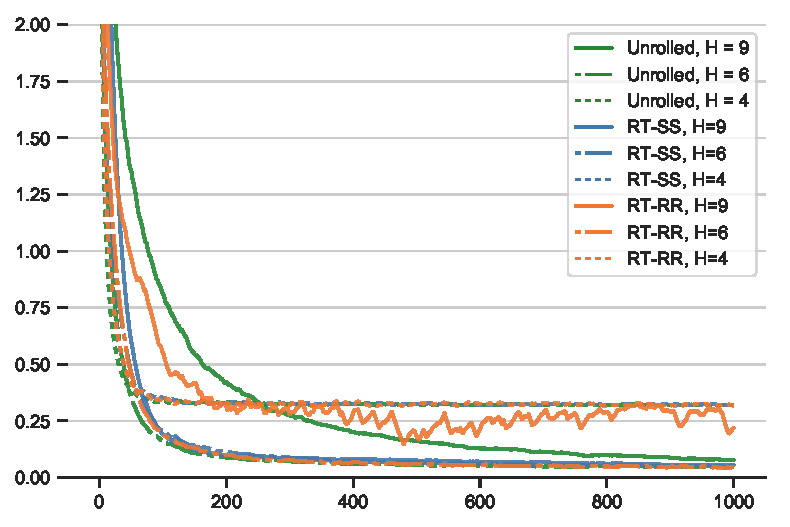
\includegraphics[width=0.9\linewidth, clip, trim=2mm 2mm 0cm 0cm]{rt/plots/lv_sgd_new/test_horizon_loss.pdf} \vspace{-1mm} \\
& \vspace{-2mm} Gradient evaluations (000s)
\label{fig:lv_loss}
\end{tabular}
\caption{Lotka-Volterra parameter inference}
\vspace{-0.5cm}
\end{figure}

Figure \ref{fig:lv_loss} shows the loss of the different estimators over the course of training.
RT-SS estimators outperform the un-truncated estimator without inducing bias.
They are competitive with the truncation~${H = 6}$, while avoiding the bias present with the truncation~${H = 4}$.
By contrast, some RT-RR estimators experience issues with optimization, falling into the same local minimum as the $H = 4$ truncation.

\subsection{MNIST learning rate}
We next experiment with meta-optimization of a learning rate on MNIST.
We largely follow the procedure used by \cite{wu2018understanding}.
We use a feedforward network with two hidden layers of 100 units, with weights initialized from a Gaussian with standard deviation 0.1, and biases initialized to zero.
Optimization is performed with a batch size of 100.

The neural network is trained by SGD with momentum using Polyak averaging, with the momentum parameter fixed to $0.9$.
We aim to learn a learning rate $\eta_0$ and decay $\lambda$ for the inner-loop optimization.
These are initialized to $0.01$ and $0.1$ respectively.
The learning rate for the inner optimization at an inner optimization step $t$ is~$
{\eta_t = \eta_0(1 + \frac{t}{5000})^{-\lambda}}$.

As in \cite{wu2018understanding}, we pretrain the net for 50 steps with a learning rate of $0.1$.
$\mathcal{L}_n$ is the evaluation loss after $2^n + 1$ training steps with a batch size of $100$.
The evaluation loss is measured over $2^n + 1$ validation batches or the entire validation set, whichever is smaller.
The outer optimization is performed with a learning rate of $0.01$.

RT estimators with $H = 9$ or $H = 5$ achieve faster convergence than the fixed-truncation estimators.
RT-SS outperforms RT-RR.
All estimators with $H = 5$ appear to suffer from some bias.
The un-truncated estimator achieves a slightly better loss than the RT estimators, but takes significantly longer to converge.

\begin{figure}
\vspace{-0.3cm}
\small
\begin{tabular}{c c}
\rotatebox{90}{\qquad\qquad$\text{Evaluation loss}$}&
\hspace{-2mm}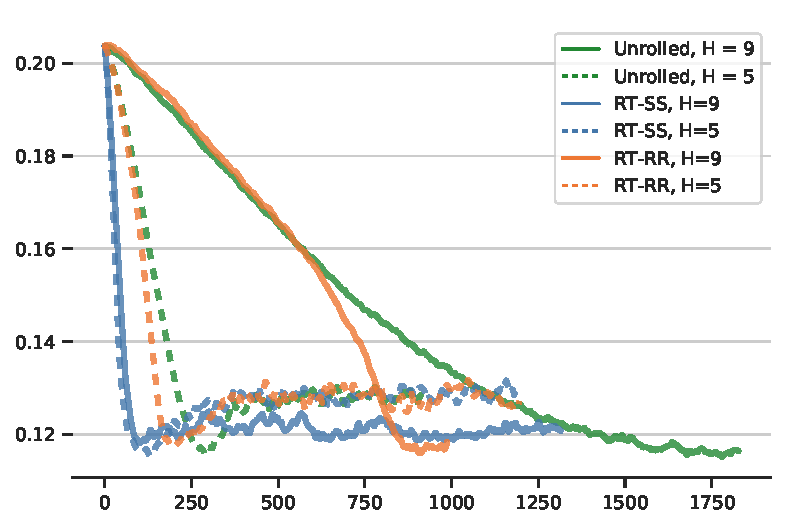
\includegraphics[width=0.9\linewidth, clip, trim=2mm 2mm 0cm 0cm]{rt/plots/mnist_sgd/fullhorizon_eval_cross_entropy.pdf} \vspace{-1mm} \\
& \vspace{-2mm} Neural network evaluations (000s)
\label{fig:mnist_loss}
\end{tabular}
\caption{MNIST learning rate meta-optimization}
\vspace{-0.1cm}
\end{figure}

\subsection{\texttt{enwik8} LSTM}
Finally, we study a high-dimensional optimization problem:
training an LSTM to model sequences on $\texttt{enwik8}$.
These data are the first 100M bytes of a Wikipedia XML dump.
There are 205 unique tokens. We use the first 90M,
5M, and 5M characters as the training, evaluation, and test sets.

We build on code from
\cite{merity2017regularizing, merity2018analysis} found at
https://github.com/salesforce/awd-lstm-lm. We train
an LSTM with 1000 hidden units and 400-dimensional input and output
embeddings. The model has 5.9M parameters. The only regularization is
an $\ell_2$ penalty on the weights with magnitude $10^{-6}$.
Gradients are clipped to magnitude $1.0$ before each optimization step.
The optimization is performed with a learning rate of $2.2$.
This model is not state-of-the-art: our aim to investigate performance of
RT estimators for optimizing high-dimensional neural networks, rather than to
maximize performance at a language modeling task.

We choose $\mathcal{L}_n$ to be the mean
cross-entropy after unrolling the LSTM training for $6 * 2^n + 1$ steps.
We choose the horizon $H = 5$, such that
the un-truncated loop has 193 steps, chosen to be approximately equal to the
200-length training sequences used by \cite{merity2018analysis}.

Figure \ref{fig:enwik} shows the training bits-per-character (proportional to the training cross-entropy loss).
All RT estimators provide some acceleration over the un-truncated~${H=5}$ estimator early in training.
RT-SS underperforms relative to RT-RR.
Within the first 100k cell evaluations, the RT estimators fall back on the un-truncated estimator,
subsequently progressing slightly more slowly due to computational cost of tuning.
We conjecture that the covariance assumptions in Section 5 are often unsuited to high-dimensional problems, and lead to overly conservative estimators.

\begin{figure}
\vspace{-0.3cm}
\small
\begin{tabular}{c c}
\rotatebox{90}{\qquad$\text{Training bits-per-character}$}&
\hspace{-2mm}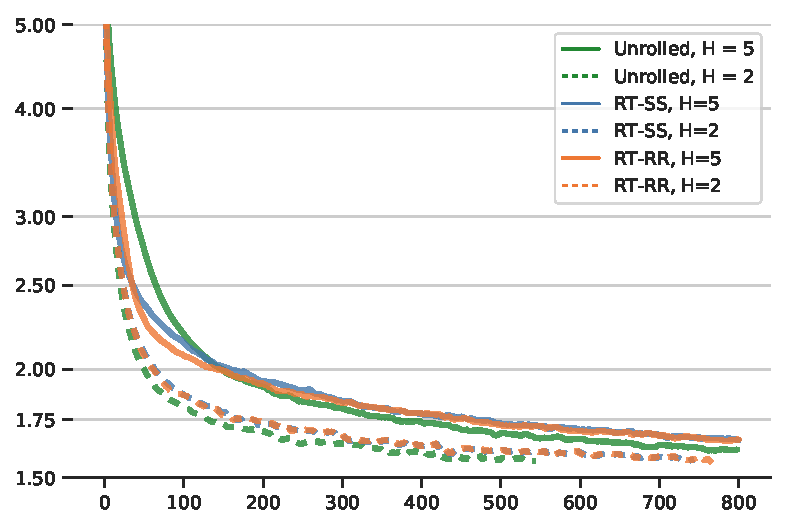
\includegraphics[width=0.9\linewidth, clip, trim=2mm 2mm 0cm 0cm]
{rt/plots/enwik_sgd/train_bpc.pdf} \vspace{-1mm} \\
& \vspace{-2mm} LSTM cell evaluations (000s)
\label{fig:enwik}
\end{tabular}
\caption{LSTM training on \texttt{enwik8}}
\vspace{-0.1cm}
\end{figure}


\section{Limitations and future work}
\textbf{Other optimizers}.
We develop the lower bound on expected improvement for SGD.
Important future directions would investigate adaptive and momentum-based SGD methods such as Adam \citep{kingma2014adam}.

\textbf{Tuning step}.
Our method includes a tuning step which requires computation.
It might be possible to remove this tuning step by estimating covariance structure online using just the values of $\hat{G}$ observed during each optimization step.

\textbf{RT estimators beyond RT-SS and RT-RR}.
There is a rich family defined by choices of $q$ and $W(n, N)$.
The optimal member depends on covariance structure between the $G_i$.
We explore RT-SS and RT-RR under strict covariance assumptions.
Could we relax these assumptions and derive or optimize approximately optimal estimators across the wider family?
This could improve adaptive estimator performance for high-dimensional problems such as training RNNs.

\textbf{Predictive models of the sequence limit}.
Using any sequence $G_n$ with RT yields an unbiased estimator as long as the sequence is consistent, i.e. its limit $G$ is the true gradient.
Combining randomized telescopes with predictive models of the gradients \citep{jaderberg2017decoupled, weber2019credit} might yield a fast-converging sequence, leading to estimators with low computation and variance.


\section{Conclusion}
We investigated the use of randomly truncated unbiased gradient estimators for
optimizing objectives which involve loops and limits.
We proved these estimators can achieve
horizon-independent convergence rates for optimizing loops and limits.
We derived adaptive variants which can be tuned online
to maximize a lower bound on expected improvement per unit
computation. Experimental results matched theoretical intuitions that the
single sample estimator is more robust than Russian roulette for optimization.
The adaptive RT-SS estimator often significantly accelerates
optimization, and can otherwise fall back on the un-truncated estimator.


\chapter{Meta-PDE: Learning to solve PDEs quickly without a mesh}

\section{Abstract}
Partial differential equations allow us to
model and design a wide variety of systems.
Solving PDEs with finite element methods
can be computationally prohibitive,
and when optimizing a design or fitting a PDE model to data,
the PDE must be solved for many different values of parameters controlling governing equations, boundary conditions, or geometric domains,
as is often the case when solving time-stepping dynamics problems or optimization problems.
Surrogate models allow fast approximate PDE solving, but existing surrogates
require fixing a vector representation for the PDE's factors of variation
(including governing equations, geometry, and boundary conditions) and for its
solution.
This makes it difficult to use surrogates
where the PDEs we encounter may have complex and varying geometry,
often requiring different meshes and representations for each problem.
Meanwhile, neural networks have drawn interest as a basis to solve PDEs
as they do not require a mesh and allow conditioning on observed data or measurements
via combining a governing equation loss with a supervised loss,
but they take far too long to optimize to be competitive with finite-element methods.

We use meta-learning to allow an alternative API for surrogate modeling.
Our model, Meta-PDE, takes as input a sampler for points in the PDE domain and
a variational energy density which measures deviation of a
given solution from the governing equations at a given point.
We use a neural network to represent the solution field, and train an initialization such that
it can quickly minimize the variational energy after a few stochastic gradient steps.
This functional API does not require fixing a parametric basis for the geometry or
governing equations.
It also does not require generating supervised data by
querying expensive finite element solvers.
We demonstrate Meta-PDE on a nonlinear Poisson problem and a nonlinear stokes
fluid-flow equation, and show it can amortize PDE solving
across different boundary conditions, governing equations,
and problem geometries.
The resulting meta-models can solve these PDEs faster than FEA,
and many orders of magnitude faster than by
training a neural network for a single PDE.

% Feedback
% \begin{itemize}
 % \item abstract higher level
%  \item mention dynamics problems as motivation
%  \item mention meshfree methods in intro
%  \item collocation methods -- meshfree
%  \item show point sampling for different domains
%  \item monte carlo variance vs geometric error
%  \item geometries not represented by vectors --
%  varying topology;
%  shape-as-program;
%  \item sampling points on boundary: programmatic
%\end{itemize}
\section{Introduction}
\label{sec:metapde-intro}
Partial differential equations (PDEs) can be used to model many
physical, biological, and mathematical systems, including those governing
thermodynamics, continuum mechanics, and electromagnetism, and have applications
outside physics in areas such as modeling populations, traffic,
optimality of continuous control, and financial markets.
Analytical solutions are rarely available for PDEs of practical importance;
thus, computational methods to approximate PDE solutions are critical for many problems in science and engineering.
One of the most widely used is finite element analysis (FEA).
In FEA, the continuous problem is discretized, with the solution represented by a
piecewise polynomial on a mesh.

Solving PDEs with FEA can be computationally prohibitive, particularly when the problem
geometry requires use of a fine mesh, as the size of the system to be solved grows
proportional to the number of mesh cells.
The computational expense is exacerbated for parameter identification or design
optimization.
In this case, the PDE must be solved at each step of a procedure optimizing some set of
design or system parameters to maximize a design objective or minimize discrepancy of
the solution from data.
Given a solution to the PDE, the \emph{adjoint method}
\citep{lions1971optimal,mitusch2019dolfin} may be used to obtain the gradient of
an objective computed from the solution with respect to the PDE parameters with cost
equivalent to a single solve of the \emph{linearized} PDE.
Therefore, the key bottleneck to optimization of PDE parameters is the "forward pass"
of obtaining an accurate solution.

\emph{Surrogate modeling} typically involves fitting a model to map from PDE parameters
in a vector basis to coefficients of an approximate solution in another vector basis.
The model is trained on a distribution of PDEs to correctly predict their solution
or to satisfy the associated PDE constraints.
These bases are fixed across the class of problems to be amortized.
However, different problems may require different meshes to represent the solution,
source terms, or boundary conditions, or may demand different representations
for the geometry itself.
Even generating a mesh which can adequately represent the geometry and solution
of a single problem can be difficult.
Surrogate modeling approaches are usually therefore restricted to scenarios where we
can fix a mesh or at least represent geometry, parameters, and solution with
fixed coefficient vectors.

Meanwhile, neural networks have long been researched as a basis with which
to solve PDEs, and have seen considerable recent interest.
Mesh-free methods such as neural networks remove some of the difficulties with
generating meshes and bases to model complex geometry.
Neural networks also allow blending observations with PDE constraints to approximate
a solution field even when the data does not come in a form amenable to being
imposed as boundary conditions \citep{raissi2019physics}.
However, neural networks take far too long to optimize to fit a given PDE to
be competitive with finite-element methods.

We use meta-learning to accelerate fitting neural networks to satisfy PDE constraints.
This lets us develop a new, "functional" API for surrogate modeling, which can handle
arbitrary geometries and removes the need to fix a mesh or to fix vector bases for the
PDE parameters or solution.
For a given PDE, our surrogate model takes as input
(i) samplers which can sample points uniformly on each region of the domain, and
(ii) a loss function encoding the PDE constraint or boundary condition for each such region.
Combining these allows unbiased estimation of a variational energy which measures
deviation of a given solution field from the governing equations.
We use a neural network to model the solution field, and train a neural network
initialization to converge quickly across a distribution of tasks
a la MAML, \citet{finn2017model}; in our case each task in the distribution
is minimizing the variational energy for a PDE with given domain, boundary
conditions and governing equations.

Our scheme has several important properties.
It does not require supervised data provided by expensive PDE solvers.
It does not place any assumptions on the structure of the geometry, and does not
require geometry to be fixed across PDEs or for the user to define a parametric
representation of varying geometry.
Similarly, it does not place any assumptions on the structure of the PDE constraints and
boundary conditions.
Geometry and governing equations are free to vary as long as the user can supply an
appropriate sampler or loss function.
It also provides the first way to train a neural network to satisfy a PDE
with competitive or faster speed to finite element analysis.

\section{Finite element analysis}
\label{sec:metapde-fea}
PDEs are most naturally posed in a \emph{strong form}:
\begin{align}
\mathcal{F}(u)(x) &= 0 \quad &\text{in } \Omega, \label{eq:metapde-strongform} \\
\mathcal{G}(u)(x) &= 0 \quad &\text{on } \partial \Omega. \label{eq:metapde-bc}
\end{align}
where $\Omega \subset \mathbb{R}^{d_\Omega}$ is the problem domain with boundary $\partial \Omega$, $u: \Omega \to \mathbb{R}^{d_u}$
is the solution,
$\mathcal{F}: (\Omega \to \mathbb{R}^{d_u}) \to (\Omega \to \mathbb{R}^{d_\mathcal{F}})$
is a linear or nonlinear operator involving $u$ and its
partial derivatives, and
$\mathcal{G}: (\Omega \to \mathbb{R}^{u}) \to (\Omega \to \mathbb{R}^{d_\mathcal{G}})$
is an operator enforcing a boundary condition
(for example, $\mathcal{G}(u)(x) = u(x) - b(x)$ is a Dirichlet boundary condition
forcing $u$ to be equal to a function $b$ on the boundary).

Finite element analysis involves rewriting the PDE in a \emph{weak form}:
find $u$ in a function space $\mathcal{V}$, such that
\begin{align}
\int_{\Omega} <\mathcal{F}(u)(x), v(x)> dx + \int_{\partial \Omega} <\mathcal{G}(u)(x), v(x)> dx &= 0 \quad \forall v \in \mathcal{V} \label{eq:metapde-eakform}
\end{align}
When $\mathcal{V}$ is a suitable infinite-dimensional Sobolev space,
we recover the same solution as the strong form.
In order to solve the problem numerically with FEA,
we let $\mathcal{V}$ be a class of piecewise low-degree polynomials over the domain,
parameterized by some finite number of interpolating points.
We fix the values of the interpolating points on the boundary, form a set of basis
vectors $v$ for $\mathcal{V}$, rewrite the weak form of the PDE as a linear or
nonlinear system representing the set of constraints that must be satisfied,
and solve the system with an appropriate linear or nonlinear solver.
Figure \ref{fig:metapde-poisson} shows as an example the Poisson problem on a disc.
For this simple problem we have $\mathcal{F}(u) = \nabla \dot{} \nabla u - f$, for
a spatially varying source term $f$, and $\mathcal{G}(u) = u$, i.e. enforcing $u=0$
on the boundary.

\begin{figure}[t]
  \centering
\includegraphics[width=10cm]{meta-pde/figures/poisson_equation.pdf}
\caption{\small Poisson equation on a disc.
Figure: \citet{xue2020amortized}.}%
\label{fig:metapde-poisson}%
\end{figure}

We observe that finding the solution to the PDE i equivalent to finding
the minimizer of the variational energy
\begin{align*}
  \mathcal{J}(u) &= \int_{\Omega} ||\mathcal{F}(u)(x)||^2_2 dx +
  \int_{\partial\Omega} ||\mathcal{G}(u)(x)||_2^2 dx
\end{align*}
As with \citet{xue2020amortized}, we use this optimization perspective
to derive an efficient training method for our surrogate models.

\section{Surrogate modeling}
Meta-PDE is a surrogate modeling approach.
Surrogate models are useful when one will need to evaluate the solution of many
PDEs from a similar family and is willing to pay the up-front cost of training a
surrogate in order to solve the downstream probelms with minimal cost-per-PDE.
The most popular application is in design or system identification, where a PDE
must be solved at each step optimizing the PDE's parameters, boundary conditions, or geometry,
and it is convenient to replace the PDE solver with a cheap surrogate~\citep{kochenderfer2019algorithms}.
The optimization may be numerical ("PDE-constrained optimization") or by hand.
If numerical, gradients can be obtained using the adjoint method with cost equivalent
to one solve of a linearized version of the PDE.
In both cases, therefore, the optimization bottleneck is in the "forward pass" of solving the PDE.
Surrogate models are also particularly relevant in scenarios involving dynamics models
(where a PDE must be solved at each timestep),
and where real-time analysis is required for the convenience of a human designer or
to allow embedding the PDE solver in a control policy.

There are many approaches to surrogate modeling, such as
random forests~\citep{criminisi2011decision},
Gaussian processes~\citep{shahriari2015taking},
Student-$t$ processes~\citep{shah2014student},
and neural networks~\citep{snoek2015scalable}.
Regression can be from the PDE's parameters to coefficients of the PDE solution,
yielding a general-purpose surrogate for that distribution of PDEs, or from
PDE parameters to an objective value for a specific optimization problem.
Most surrogate modeling procedures have two key restrictions:
\begin{enumerate}
  \item They require supervised training data in the form of
  (PDE parameter, PDE solution) or (PDE parameter, objective value) pairs,
  which must be generated by an expensive ground-truth PDE solver, \label{itm:supervision}
  \item They regress from a vector representation of the PDE or its parameters to a
  vector representaion of the solution; having to fix these vector bases
  makes it difficult to fit surrogates for
  distributions of PDEs containin highly varied structure in geometry or governing
  equations.\label{itm:structure}
\end{enumerate}
Restriction \ref{itm:supervision} means that in order to be of net computational benefit,
the surrogate must be applied to many more downstream problems than the number of
data points required to fit a good model. For rich classes of PDEs and expressive models,
it can take tens or hundreds of thousands of data points to fit a model which can generalize,
so this greatly limits surrogate models' use case.

Restriction \ref{itm:structure} is not an issue if the problem can be phrased as
regressing from coefficients of a parameter or boundary condition in a piecewise polynomial
basis to coefficients of a solution in a similar basis, with the discretization
fixed across problems.
However, many problems are not amenable to such framing.
Problems with different domain geometry or very different parameters and solutions
may require very different discretizations to represent them well;
generating a good mesh for a given problem can itself be a hard problem and can be a
greater bottleneck than the cost of the base PDE solve.
The factors of variation of a PDE (the domain, governing equations, and parameters)
are naturally and generally expressed as functions on the domain and as
operators on solutions: requiring them to be parameterized by vectors restricts
the classes of PDEs to which surrogate models can be applied and greatly limits their
use case.

Several recent works have relaxed one of these restrictions.
\citet{zhu2019physics} amortize the finite differentce method,
predicting PDE solutions from parameter fields with a
ConvNet by training the ConvNet to produce solutions with minimum variational energy
across a distribution of problems.
This removes restriction \ref{itm:supervision} but requiring the discretization
to be a fixed uniform grid.
\citet{xue2020amortized} amortize the finite element method, training a surrogate model
to minimize a similar variational energy but use a finite element discretization:
their model can handle complicated geometry, and by measuring the variational energy
in the finite element basis maintains some desirable properties of finite element
analysis. This avoids restriction \ref{itm:supervision} and allows arbitrary
meshes but requires a single mesh be fixed for all PDEs in the distribution to be
amortized.
Graph Neural Network based approaches \citep{sanchez2020learning,pfaff2020learning},
which learn a forward operator in terms of
interactions between nearby particles or mesh cells,
allow for arbitrary geometries (partially removing restriction
\ref{itm:structure})
but require supervised data and have not yet produced surrogate models which are
cheaper to evaluate than ground-truth solvers when tested on equivalent hardware.
Neural Operator based approaches \citep{li2020neural,li2020fourier} learn a map from
initial conditions or parameters to solution which builds in
some invariance to mesh \emph{resolution}, but require the mesh to be a uniform
grid, and also require expensive supervised data.

% \section{Solving PDEs with neural networks}
% \begin{itemize}
%  \item NN bases: mesh-free; instead of needing to generate a mesh,
%  need to provide a sampler and loss function. Sometimes easier
%  than generating a good discretization.
 % \item Physics-informed NNs: given known governing equations
% and some supervised data, fit a NN solution which incorporates both.
% More flexible than PDE-CO on boundary conditions to fit the data.
% \item But solving PDEs with NNs is super slow.
% \end{itemize}

\section{Meta-learning mesh-free PDE operators}
We propose Meta-PDE, an approach which meta-learns mesh-free PDE operators and
provides a new, functional API for PDE surrogate modeling.
Most PDEs can be fully defined by specification of:
\begin{itemize}
  \item a domain $\Omega$ with boundary $\partial \Omega$,
  \item an operator $\mathcal{F}$ representing governing equations,
  \item and an operator $\mathcal{G}$ representing boundary conditions.
\end{itemize}
We aim for a surrogate model with an input schema as close to this general specification as possible.
Meta-PDE uses meta-learning, and specifically MAML \citep{}, to achieve this.
Meta-PDE's parameters are the initial parameters $\theta_0$ for a neural network
$u_\theta$ representing
a function $u: \mathbb{R}^{d_\Omega} \to \mathbb{R}^{d_u}$,
and per-parameter per-step learning rates $\alpha_k$.
The geometric dimension $\mathbb{R}^{d_\Omega}$ and solution dimension $\mathbb{R}^{d_u}$
must remain fixed across PDEs in the distribution, even though $\Omega$ is allowed to vary.
When using Meta-PDE as a surrogate to compute an approximate solution to a given PDE
(one 'example' or 'task'),
the inputs to the Meta-PDE model are:
\begin{itemize}
  \item a sampler $s(\Omega)$ which returns points in the domain $\Omega$,
  \item a sampler $s(\partial\Omega)$ which returns points on the boundary $\partial\Omega$,
  \item an operator $\mathcal{F}$ representing governing equations,
  \item and an operator $\mathcal{G}$ representing boundary conditions.
\end{itemize}

The operators $\mathcal{F}$ and $\mathcal{G}$ may be supplied directly and do not
require a particular parametric form.
The user must supply a sampler for the domain and for the boundary of each PDE within
the training distribution and for each PDE seen during deployment.
A sampler can easily be constructed for any domain for which we have a mesh,
but it is also often easier to construct a sampler than to construct an accurate mesh.
Finite element models usually use piecewise linear meshes, which can take many elements
to accurately represent curved shapes: even when using piecewise polynomially-shaped meshes,
the slow rate of convergence of using these meshes to approximate
non-polynomial geometry can be a major source of error and/or computational expense
for FEA.
Given an inside-outside oracle for the domain, it is easy to use rejection sampling
to sample from it exactly.
Most parametric geometry representations such as those used
in computer-aided design also allow exact sampling of the boundary, and even
minimal representations such as signed distance functions allow approximate
sampling \citep{brubaker2012family}.

The samplers and operators are sufficient to construct an estimator $\hat{\mathcal{J}}$ for the variational
energy $\mathcal{J}$:
\begin{align*}
  \mathcal{J}(u) &= \int_{\Omega} ||\mathcal{F}(u)(x)||^2_2 dx +
  \int_{\partial\Omega} ||\mathcal{G}(u)(x)||_2^2 dx \\
  \hat{\mathcal{J}}(u) &= \mathbb{E}_{x \sim s(\Omega)} ||\mathcal{F}(u)(x)||^2_2 +
  \mathbb{E}_{x \sim s(\partial \Omega)} \int_{\partial \Omega} ||\mathcal{G}(u)(x)||_2^2
\end{align*}
$\hat{\mathcal{J}}(u)$ is unbiased as long as $s(\dot{})$ return points with
uniform probability over their supports, or return batches of points which have uniform
probability for any given $x$ aggregated over the batch. Unbiased estimation is not
necessarily essential. Note $\hat{\mathcal{J}}(u) > 0$ and $\mathcal{J}(u) > 0$
$\forall u$, and the true solution $u^*$ of the PDE achieves
$\mathcal{J}(u) = \hat{\mathcal{J}}(u) = 0$. These properties hold if we multiply
the integrand in $\mathcal{J}(u)$ by an arbitrary density $\mu > 0$ or if we
choose samplers $s$ which have full support but nonuniform probability on $\Omega$
or $\partial \Omega$. Therefore, biased sampling will not change the minimizer of the
energy estimator if we have a sufficiently expressive hypothesis class for $u$.

The "forward pass" computing an approximate solution for a given PDE involves
a small number $K$ of inner-loop steps (we use $K=5$) of stochastic optimization,
minimizing the variational energy $\mathcal{J}(u)$ and starting from
the initialization $\theta_0$:
\begin{align*}
  \theta_k = \theta_{k-1} - \alpha_k \nabla_{\theta_{k-1}} \hat{\mathcal{J}}(u_{\theta_{k-1}}) \quad k = 1 .. K
\end{align*}

Meta-PDE returns the approximate solution $u_{\theta_K}$, the neural network
with the final set of parameters.

To train Meta-PDE, we use a distribution of tasks, each specified by
samplers and constraint operators for the boundary and loss, each representing a
different PDE.
We draw a batch of tasks with variational energy estimators $\hat{\mathcal{J}}_i$,
$i = 1 ... n$, and unroll the inner loop to find $u_{\theta_K, i}$.
For each task the loss is $\hat{\mathcal{J}}_i(u_{\theta_K, i})$.
We backpropogate through the inner loop to find the gradients
$\nabla_{\theta_0} \sum_i \frac{1}{n} \hat{\mathcal{J}}_i(u_{\theta_K, i})$
and $\nabla_{\alpha} \sum_i \frac{1}{n} \hat{\mathcal{J}}_i(u_{\theta_K, i})$,
which are used in an outer loop to train the model.

\section{Experiments}
We demonstrate Meta-PDE on a nonlinear Poisson problem with varying
source terms, boundary conditions, and geometric domain.
The PDE takes the form:
\begin{align*}
\nabla \dot{} ((1 + 0.1 u^2) \nabla u)(x) &= f(x) \quad &x \text{ in } \Omega\\
\nabla \dot{} u(x) &= b(x) \quad &x \text{ on } \partial\Omega,
\end{align*}
where $u \in \mathbb{R}^1$ and $\Omega \subset \mathbb{R}^2$.
Using our notation from the preceding section, this is equivalent to
constraining the solution in the domain with an operator~${
\mathcal{F}(u) = ((1 + 0.1 u^2) \nabla u) - f}$, and constraining
the solution on the boundary with an operator~${\mathcal{G}(u) = u - b}$.

The domain $\Omega$ is a disc-like shape centered at the origin, defined in polar coordinates by  and the varying
radius about the origin
\[
r(\theta) = r_0[1 + c_1 \cos(4\theta) + c_2 \cos(8\theta)],
\]
where the varying parameters are $c_1, c_2 \sim \mathcal{U}(-0.2, 0.2)$.
The source term $f$ is a sum of radial basis functions,
\[
f(x) = \sum_{i=1}^3 \beta_i \exp{||x - \mu_i||_2^2},
\]
where $\beta_i \in \mathbb{R}^1$ and $\mu_i \in \mathbb{R}^2$ are both drawn from
standard normal distributions.
The boundary condition $b$ is a periodic function, defined in polar coordinates as
\[
b(x) = b_0 + b_1 \cos(\theta) + b_2 \sin(\theta) + b_3 \cos(\theta) + b_4 \sin(\theta),
\]
where the parameters $b_{0:4} \sim \mathcal{U}(-1, 1)$.
%Figure \todo{make fig} shows the domain, source term, and boundary conditions across several sampled PDEs.

We train Meta-PDE with a batch size of 16 tasks, with 5 inner steps,
and with 256 sampled points on the boundary and in the domain used to evaluate the
variational energy at each inner step of optimization for each task.
To sample points on the boundary, we construct an evenly spaced interval mesh of
angles in
$[0, 2 * \pi]$, add uniform noise of the size of one interval to each point, and use
the points on the boundary using these angles.
To sample points in the domain, we do the same but also draw random radii uniformly in
$[0, r(\theta)]$.
These samplers are not unbiased for non-circular shapes,
but this does not change the optimal solution.

Our model is a three layer NN with sinusoidal activations initialized according to
the scheme in \citet{sitzmann2020implicit},
(although we replace $\omega_0 = 30.$ in that paper with $\omega_0 = 3.$
to avoid numerical issues when taking higher-order derivatives of
a neural network's input-output function).
We initialize the inner-loop learning rate to $1\times 10^{-4}$, and use an outer loop learning
rate of $1\times 10^{-5}$.
Gradients in both inner and outer loop are clipped to have maximal norm $100$.
In the inner loop, we use vanilla SGD.
In the outer loop, we use the Adam optimizer \citep{kingma2014adam}.
%  with lookahead \todo{cite} and the warmup schedule from \todo{cite}.
We train for 200,000 outer-loop steps, which takes about 6 hours on one
GeForce RTX 2080.

All finite element baselines are implemented in FEniCS
\citep{LoggMardalEtAl2012a,AlnaesBlechta2015a}.
We use the Mumps linear solver backend.
Meta-PDE is implemented in Jax \citep{jax2018github}.

% FENICS
% res: 1, rel_mse: 0.28237417340278625, std_rel_mse: 0.6290896534919739, time: 0.05341055989265442
% res: 2, rel_mse: 0.014543757773935795, std_rel_mse: 0.029957808554172516, time: 0.12654799222946167
% res: 3, rel_mse: 0.006523779593408108, std_rel_mse: 0.013875527307391167, time: 0.23686206340789795
% res: 4, rel_mse: 0.0011952054919674993, std_rel_mse: 0.0021807190496474504, time: 0.4497535675764084
% res: 5, rel_mse: 0.0007102875970304012, std_rel_mse: 0.0014738228637725115, time: 0.7402735650539398
% res: 6, rel_mse: 0.0003710805904120207, std_rel_mse: 0.0008687296649441123, time: 0.8322657346725464
% res: 8, rel_mse: 4.029081901535392\times 10^{-05, std_rel_mse: 5.9528952988330275\times 10^{-05, time: 1.23470838367939
% res: 10, rel_mse: 2.8872436814708635\times 10^{-05, std_rel_mse: 6.197320180945098\times 10^{-05, time: 1.8577006310224533
% res: 12, rel_mse: 5.06512105857837\times 10^{-06, std_rel_mse: 9.67413689068053\times 10^{-06, time: 2.4609854966402054

% Us
% maml_poisson_outer1en5_inner1en4_outerclip1e2_innerclip1e2
% time: 0.0022 // 0.19 s
% err: 0.00013, std 0.00027

\begin{table}
\begin{adjustbox}{max width=\textwidth}
\begin{tabular}{|c|ccccc|}
 \hline
 Method & Resolution & Mean finite element DoFs & Relative MSE & Simulation time (CPU) & Simulation time (GPU) \\
 \hline
 FEA & 1 & 15 & $0.28 \pm 0.63$ & 0.053s & N/A \\
 FEA & 2 & 53 & $0.014 \pm 0.030$ & 0.13s & N/A \\
 FEA & 3 & 85 & $0.0065 \pm 0.014$ & 0.24s & N/A \\
 FEA & 4 & 178 & $0.0012 \pm 0.0022$ & 0.45s & N/A \\
 FEA & 5 & 222 & $7.1\times 10^{-4} \pm 1.5\times 10^{-3}$ & 0.74s & N/A \\
 FEA & 6 & 324 & $3.7\times 10^{-4} \pm 8.7\times 10^{-4}$ & 0.83s & N/A \\
 FEA & 8 & 433 & $4.0\times 10^{-5} \pm 6.0\times 10^{-5}$ & 1.2s & N/A \\
 FEA & 10 & 568 & $2.9\times 10^{-5} \pm 6.2\times 10^{-5}$ & 1.9s & N/A \\
 FEA & 12 & 1246 & $5.1\times 10^{-6} \pm 9.7\times 10^{-6}$ & 2.5s & N/A \\
 FEA & 16 & 2163  & $5.1\times 10^{-6} \pm 9.7\times 10^{-6}$ & 2.92s & N/A \\
 Meta-PDE & N/A & N/A & $6.2\times 10^{-5} \pm 1.0\times 10^{-4}$  & 0.097s & 0.0022s \\
 \hline
\end{tabular}
\end{adjustbox}
\caption{
Accuracy vs solution time for finite element methods and for meta-PDE.
For FEA, a mesh is generated with MSHR using 3x "resolution" points
to define the geometry, and "resolution" as an argument to MSHR's
automeshing too.}
\label{tbl:results}
\end{table}

\begin{figure}[t]
  \centering
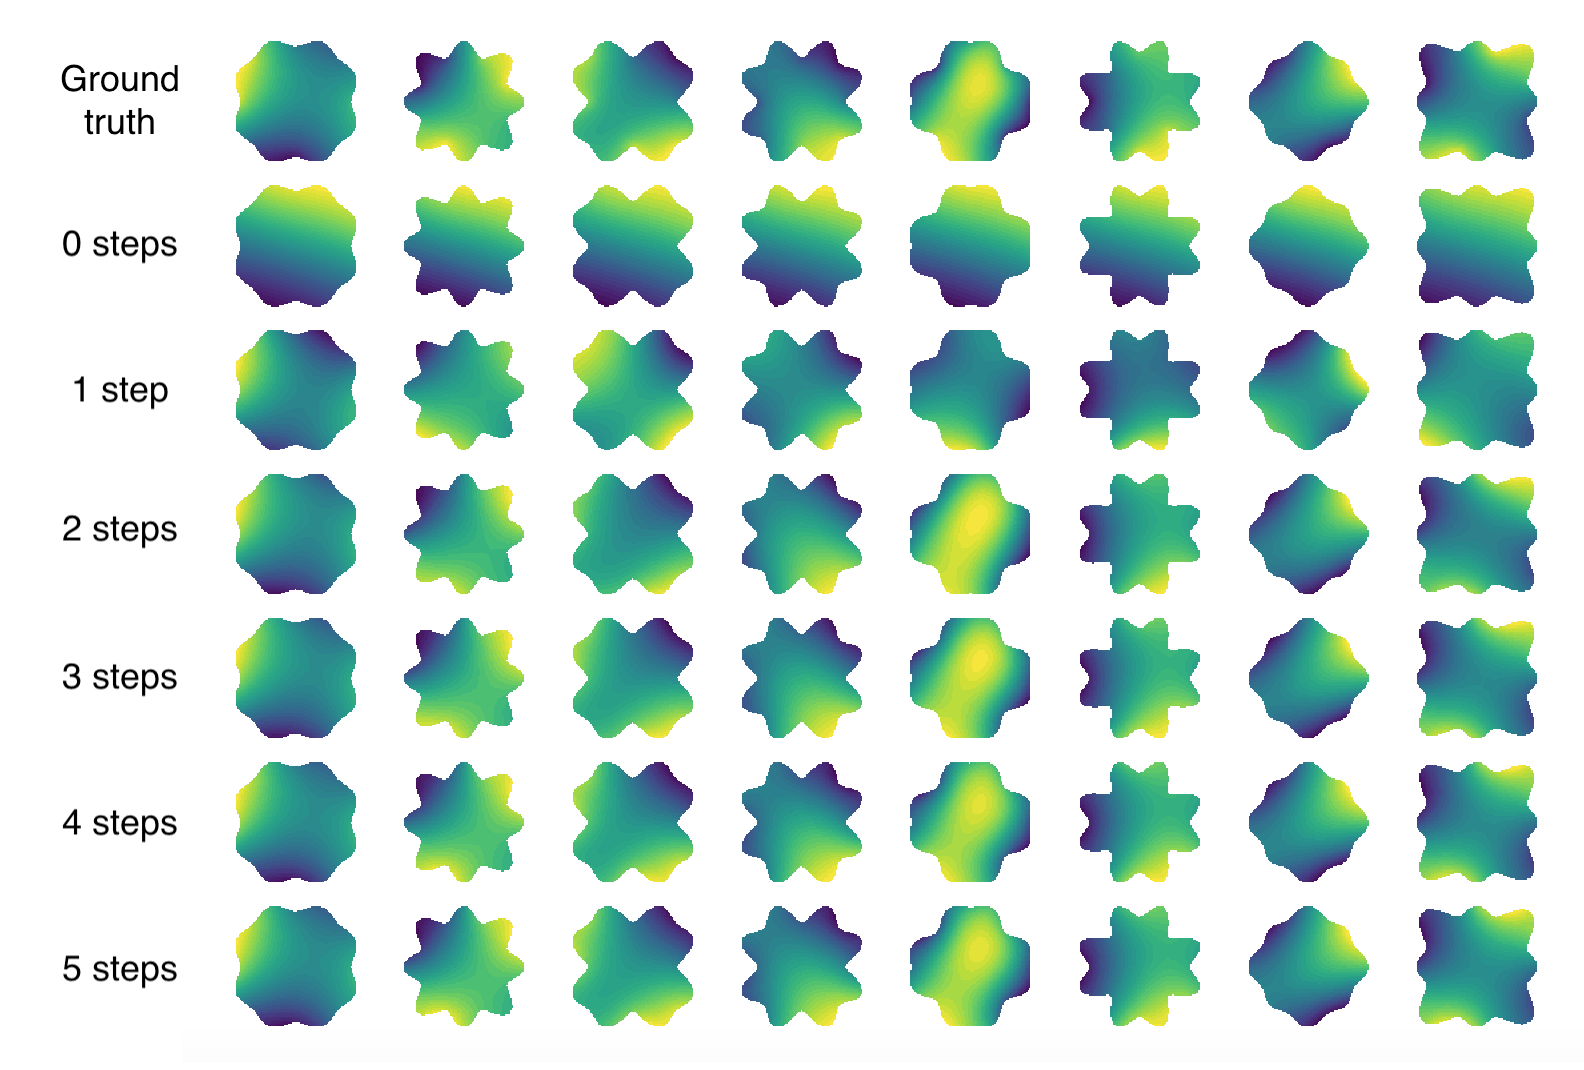
\includegraphics[width=10cm]{meta-pde/figures/poisson_meta_labeled.png}
\caption{\small
Solutions to nonlinear Poisson equations with varying domains, boundary conditions
and source terms. Top: ground truth finite element solution.
Second row: solution represented by Meta-PDE initial neural network parameters.
Third row onwards: solution after each gradient step in the Meta-PDE inner loop.}%
\label{fig:results_per_step}%
\end{figure}

Meta-PDE learns to quickly find solutions with low error. Table \ref{tbl:results}
shows the mean squared solution error and solution time after zero through five gradient steps for
a Meta-PDE model trained to minimize the energy estimate after five gradient steps,
as compared to finite element models of varying fidelities.
The highest-fidelity finite element model was taken as ground truth and was used to
compute errors.
Errors and solution times were evaluated using sixteen held-out problems from the same
distribution which were not used during training
Mean-squared errors are computed
between the value of a given approximate solution and the value of the ground truth
(highest fidelity finite element solution) at 1024 randomly sampled points within
the domain.
The relative mean-squared error is computed by dividing the mean-squared error by
the sum of squares of solution values for the ground-truth solution.
% Figure \todo{make} shows the ground truth and finite element approximations of
various fidelities for sampled test problems.
Figure \ref{fig:results_per_step} shows the ground truth and the Meta-PDE solution after
zero through five gradient steps minimizing the variational energy for
sampled test problems.


We see that Meta-PDE learns to output accurate solutions, and when run on the same
CPU (a 2.5GHz Intel i7) is about 4-7x faster than a finite element method with similar
accuracy, and about 50x more accurate than a finite element method
with the same computation cost.
Unlike finite element models, Meta-PDE can be easily accelerated by a GPU,
and on GPU we see close to 50x speed up in deployment,
leading to a 400x speed increase over similar accuracy finite element models.
We expect these gains would only increase if we replaced the vanilla fully-connected
neural network with a more tailored NN (such as the attention-like model used
to fit PDE solutions in \citet{wang2020understanding}),
used a lower-variance sampling strategy,
or more carefully tailored a meta-learning algorithm to this problem.
The speed-accuracy tradeoff could also be tuned by changing the size of the NN used
or the number of steps in the inner loop optimization.

% %\section{Discussion}

\section{Conclusion}
We presented Meta-PDE, a surrogate model uses meta-learning to amortize PDE solving
across classes of PDEs with complex and varying geometries and governing equations.
Meta-PDE takes as input the governing equations themselves and a sampler for the
PDE domain and boundary, thus remaining as close as possible in API to the fundamental
representation of the PDE in terms of governing equations and domain.
This avoids having to fix a parametric representation of geometry, governing equations
and solution for the class of PDEs to be amortized.
We show on a nonlinear Poisson problem that Meta-PDE can learn to output accurate
solutions with a significantly more favorable accuracy-speed tradeoff than
a baseline finite element solver.

\chapter{Conclusion}
In this thesis, we presented several methods using deep learning and
stochastic gradient estimation to speed up numerical modeling.
There is an increasing and justified interest in using neural networks and other
tools from the discipline of machine learning to accelerate numerical procedures
(as function approximation has been used to do for decades).
As researchers and engineers increasingly integrate machine learning into
numerical modeling, it will often be tempting to think about either machine learning
or the numerical procedure or both as a black box
-- to use a numerical method as just a source of parameter vector, solution vector
pairs for a regression dataset, or to use machine learning methods as just a tool
for doing said regression.
In certain scenarios, where data is plentiful and conforms to such a schema,
such an approach can be appropriate and can have great results.

However, going beyond this shallow approach will let us develop methods which
are of use in a far wider range of scenarios.
In this thesis, we showed that
tailoring machine learning methods to the computational and physical structure of
numerical models can let us train models on cheap simulations and deploy them
as surrogates for expensive simulations, or lets us remove the need for
supervised data entirely,
and lets us develop new efficient methods for optimization and system identification.
Perhaps most importantly, synthesis of ML and numerical modeling can allow
us to develop methods with new and more flexible APIs, and which allow acceleration of
broader classes of numerical models.
\bibliographystyle{plainnat}
\bibliography{references}


\appendix

\chapter{List of publications}
\subsection{Chapter 2}
\begin{itemize}
\item \bibentry{beatson2020learning}
\end{itemize}

\subsection{Chapter 3}
\begin{itemize}
  \item \bibentry{beatson2019efficient}
\end{itemize}

\subsection{Chapter 4}
\begin{itemize}
  \item \bibentry{beatson2021meta}
\end{itemize}

\subsection{Not included in this thesis}
\begin{itemize}
\item \bibentry{oktay2021randomized} %
\item \bibentry{xue2020amortized} %
\item \bibentry{xue2020data} %
\item \bibentry{luo2020sumo} %
\item \bibentry{ravi2018amortized} %
\item \bibentry{seff2017continual} %
\item \bibentry{beatson2016blind} %
\end{itemize}

\chapter{Appendix for Chapter 2}
\section{Contents}
This appendix consists of:
\begin{itemize}
  \item specification of the data generating distribution and hyperparameters;
  \item visualization of data generated via Hamiltonian Monte Carlo;
  \item visualization of data generated via \textsc{DAgger};
  \item hyperparameters used for neural network specification and training;
  \item ablation study of neural network design choices;
  \item specification of the finite element meshes used as baselines;
  \item visualization of all solutions found under compression and tension
  for each pore shape for each baseline mesh and the composed energy surrogate.
\end{itemize}

\clearpage
\section{Data generation with Hamiltonian Monte Carlo}
We use 100 data collectors, each with randomly drawn hyperparameters, which
each terminate (and have their place taken by a newly initialized collector)
after sampling 25 data points.
We collect 60,000 data points, consisting of a training set of 55,000 and a validation set of 5,000.
As our distribution is arbitrary, and as we assume that more data is always a good thing, when a HMC sample is rejected, we still add it to the dataset, but return to the last un-rejected sample to continue the Markov chain.

Hyperparameter distributions are chosen heuristically such that the finite element simulation tends to converge in a reasonable amount of time.
The hyperparameter distributions are as follows:

\begin{itemize}
\item Leapfrog step size: $\mathcal{U}(0.005, 0.02)$
\item Leapfrog path length: $\mathcal{U}(0.05, 0.3)$
\item Temperature used to scale the log-probability: $\mathcal{U}([0.0001,0.0005,0.001,0.005,0.01,0.05,0.1])$
\item Standard deviation of the Gaussian from which the Hamiltonian momentum is drawn: $\mathcal{U}(0.01, 0.3)$
\end{itemize}

We approximate the macroscopic strain tensor $\bar{x}$ from $\mathbf{u}$ as:

\resizebox{\linewidth}{!}{
  \begin{minipage}{\linewidth}
\begin{align*}
\bar{x}(\mathbf{u}) = \frac{1}{N} \begin{bmatrix}
\displaystyle\sum_{X \in \text{rhs}} \!\!u_1(X) \!-\!\!\! \sum_{X \in \text{lhs}} \!\!u_1(x)
&
\displaystyle\sum_{X \in \text{rhs}} \!\!u_2(X) \!-\!\!\! \sum_{X \in \text{lhs}} \!\!u_2(X)
\\
\displaystyle\sum_{X \in \text{top}} \!\!u_1(X) \!-\!\!\! \sum_{X \in \text{bot}} \!\!u_1(x)
&
\displaystyle\sum_{X \in \text{top}} \!\!u_2(X) \!-\!\!\! \sum_{X \in \text{bot}} \!\!u_2(X)
\end{bmatrix}
\end{align*}
\end{minipage}
}

Above,~$u_1(X)$ and~$u_2(X)$ are horizontal and vertical displacements defined by $\mathbf{u}$ at a point $X$, and top, bot, lhs and rhs are the set of control point locations for the splines on the top, bottom, left and right of the component.

\clearpage

\section{Visualizing HMC data}
Here we display 24 randomly chosen examples from the training set.
\begin{figure}[H]
  \centering
  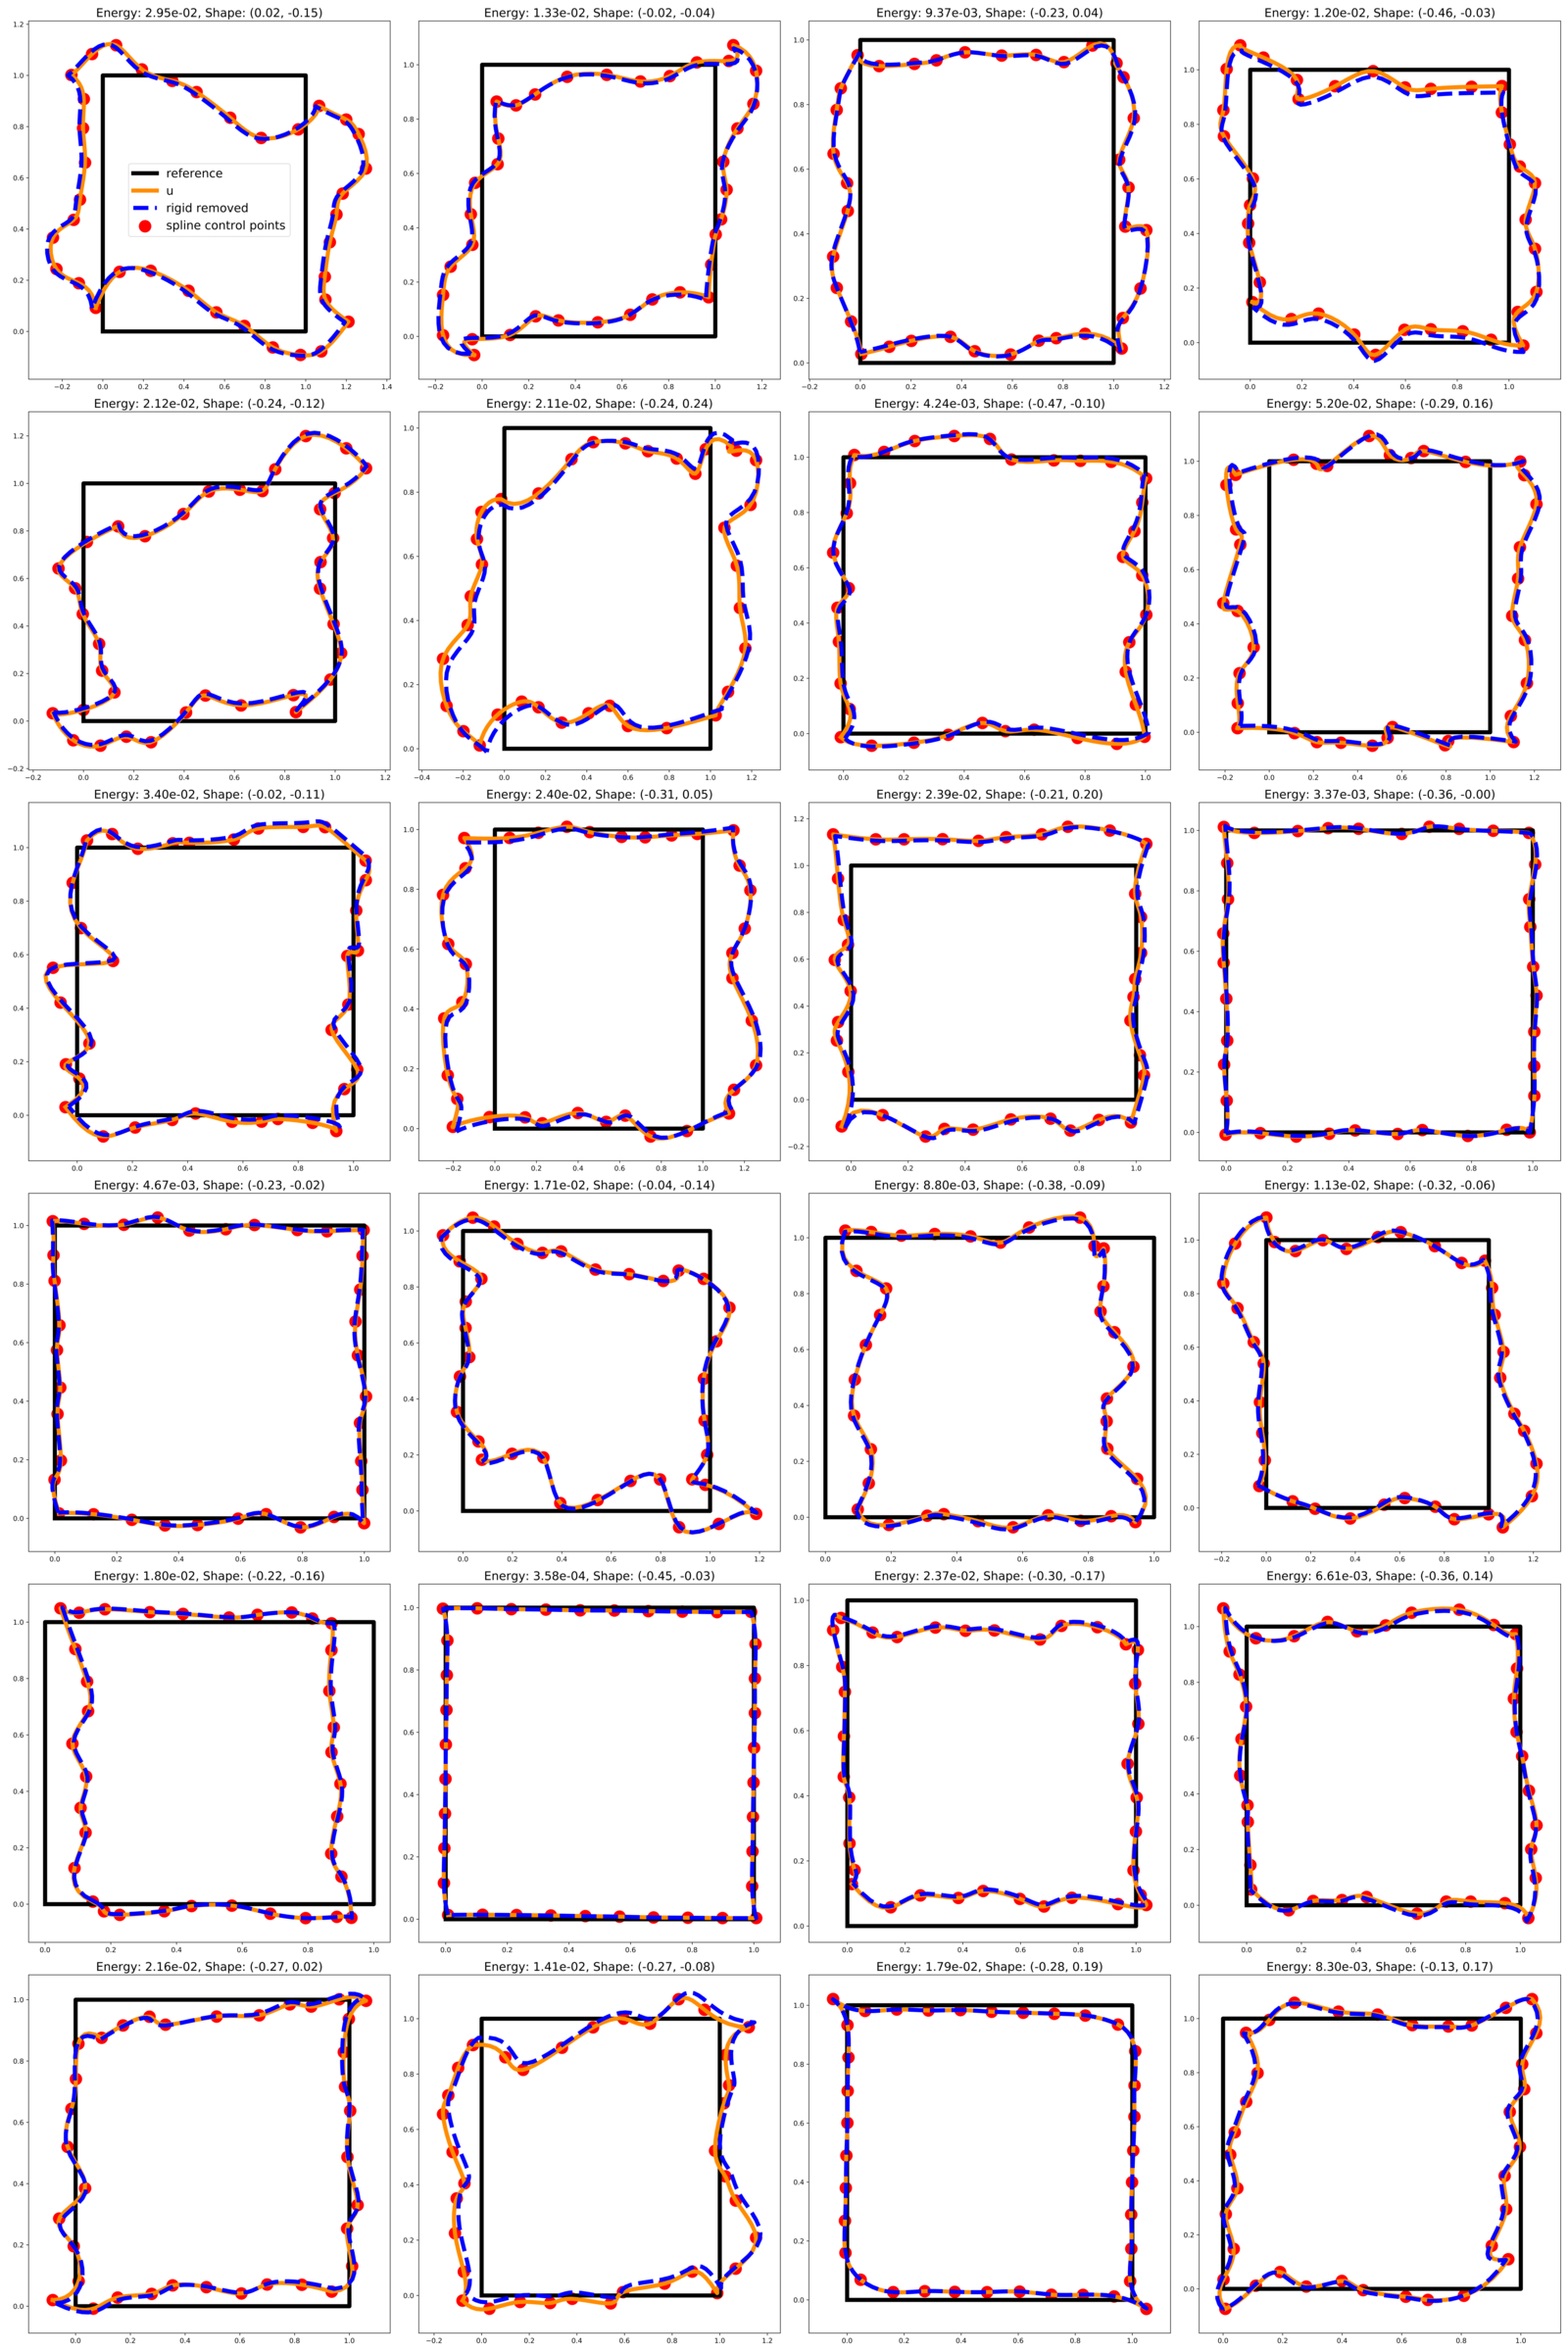
\includegraphics[width=.7\linewidth]{lces/hmc_viz.png}
\end{figure}

\clearpage

\section{Visualizing \textsc{DAgger} data}
Here we display 24 randomly chosen examples from the data collected with \textsc{DAgger}.
\begin{figure}[H]
  \centering
  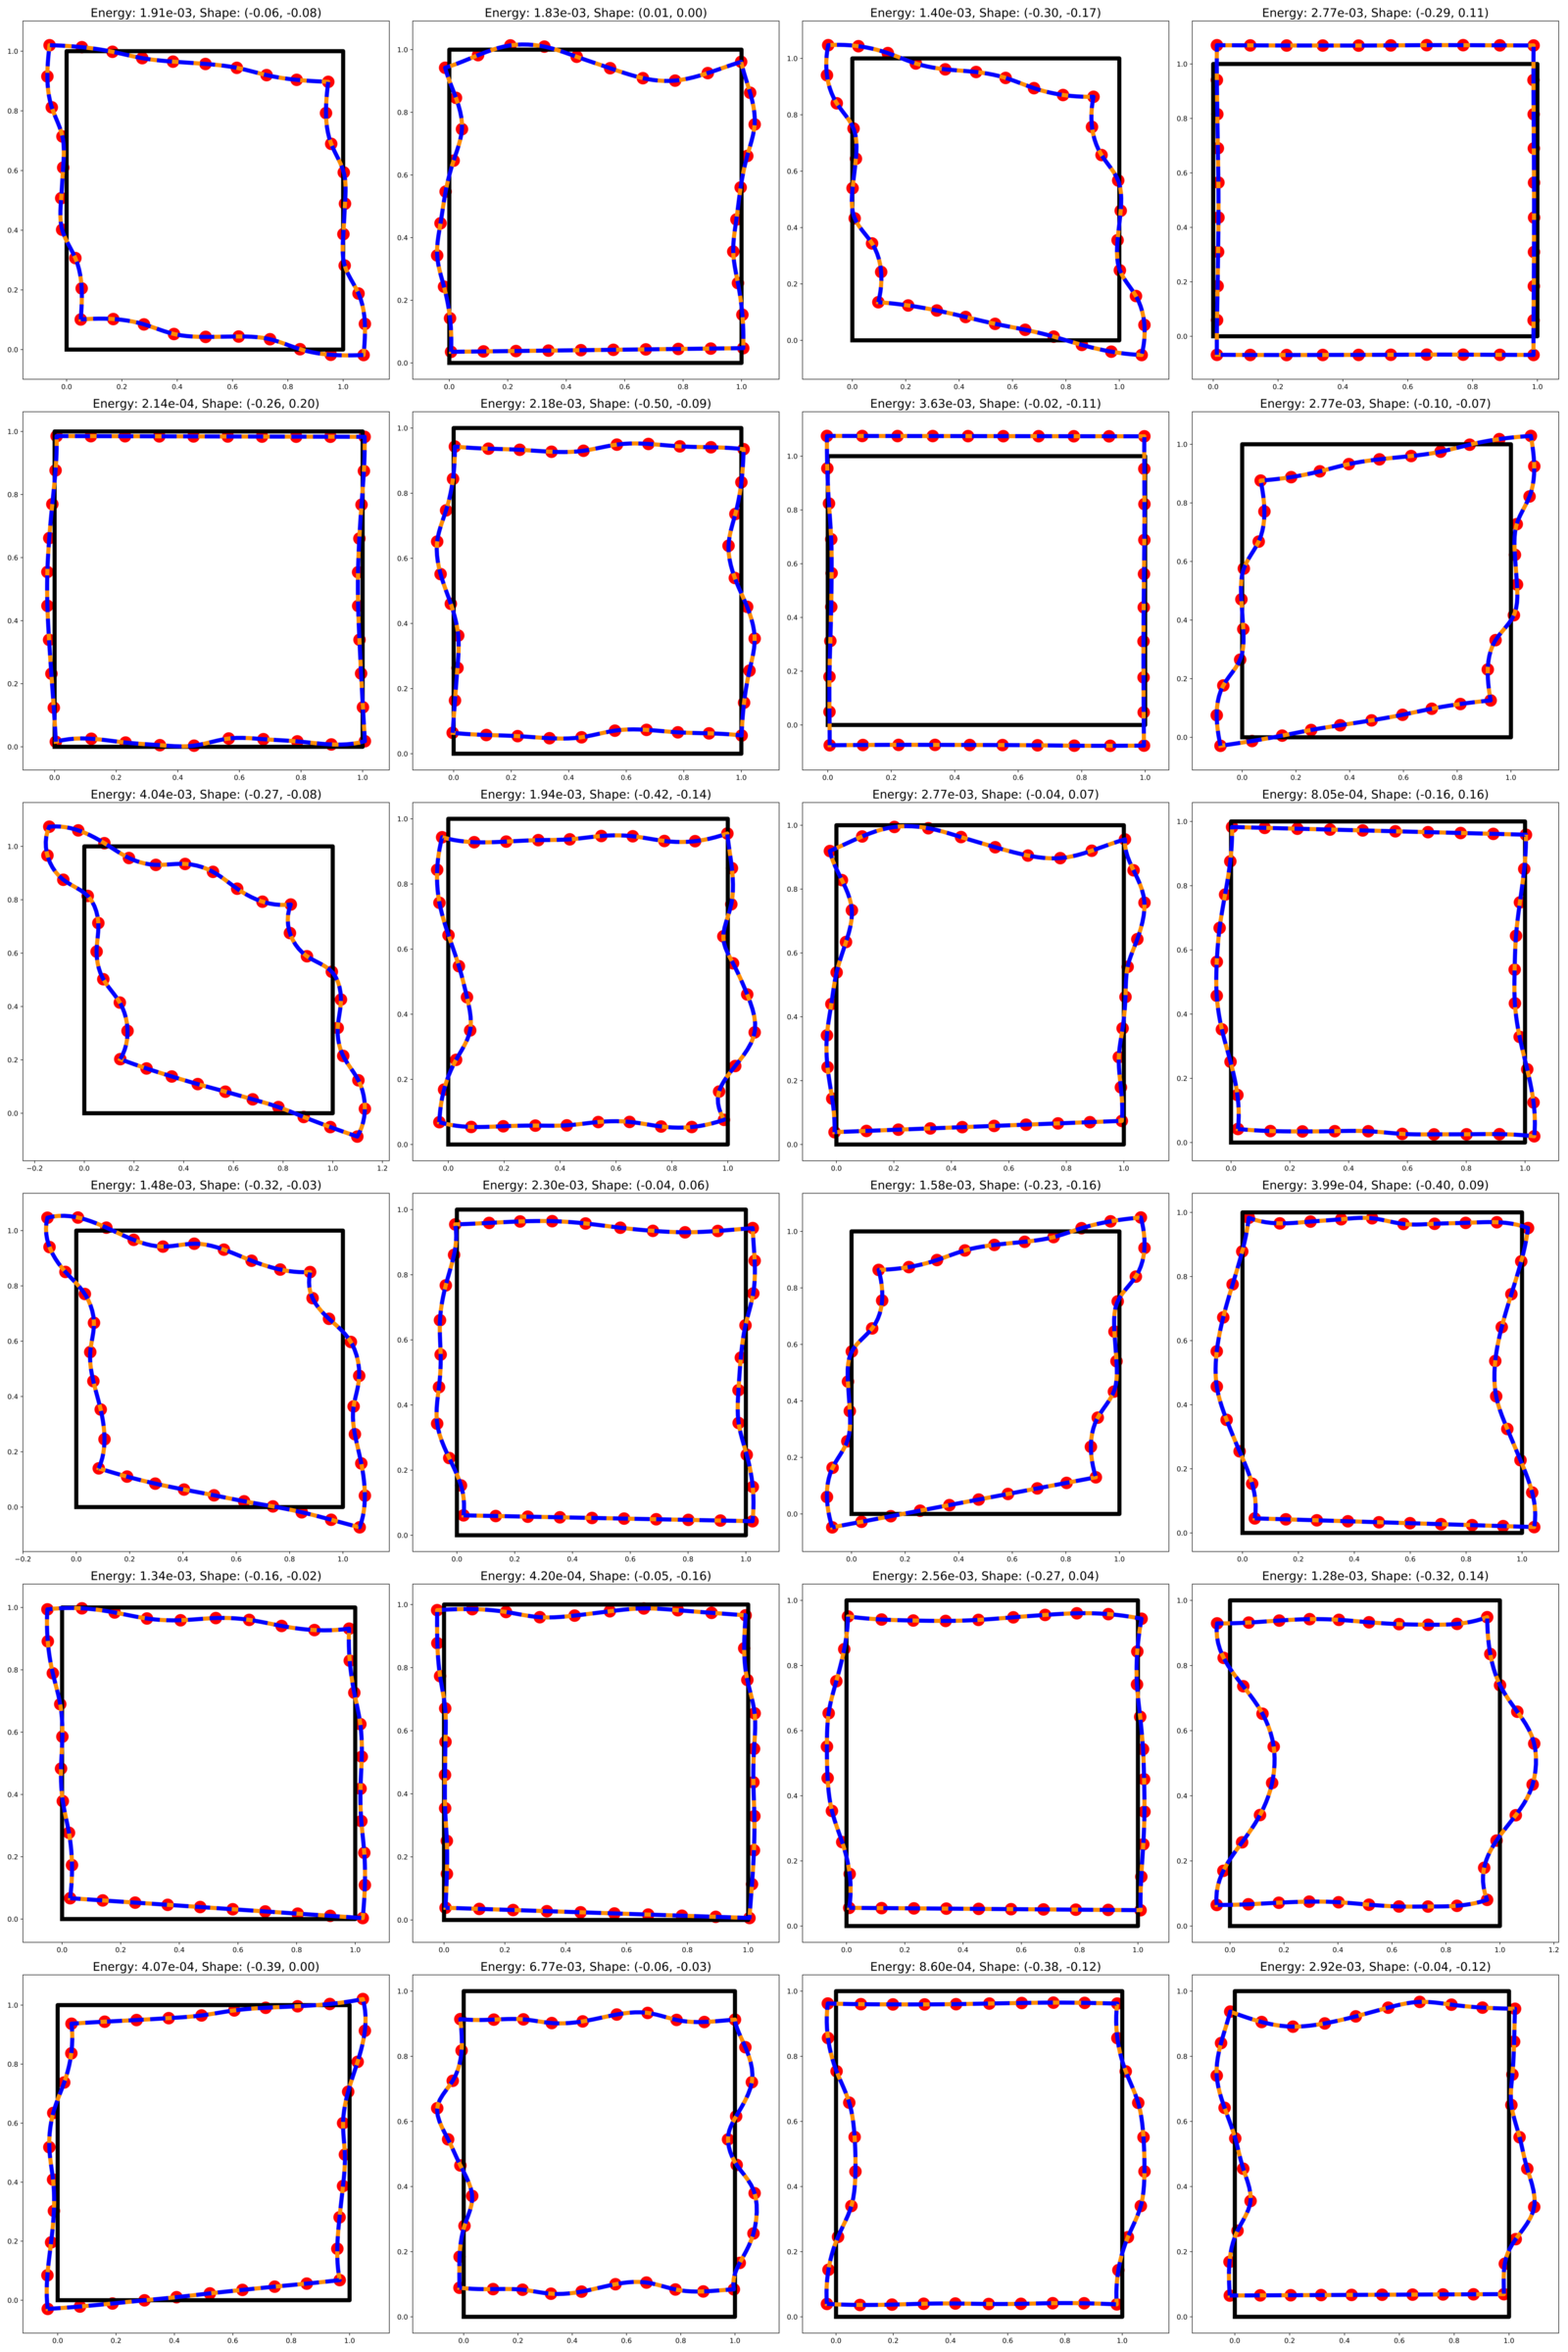
\includegraphics[width=.7\linewidth]{lces/dagger_viz.png}
\end{figure}

\section{Neural network hyperparameters}
We use a fully-connected neural network with three hidden layers of 512 units, Swish nonlinarities, and He initialization.
We optimize our neural network using Adam with a learning rate of 3e-4 and a batch size of 512.

\section{Surrogate design ablation study}
We perform an ablation study by switching on and off the following independent variables:
\begin{itemize}
\item "Scale": parameterizing the log of the scalar stiffness, vs parameterizing energy directly;
\item "Remove rigid": removing rigid body translations from the data via Procrustes analysis;
\item "Sobolev-G": Sobolev training on energy gradients;
\item "Sobolev-Hvp": Sobolev training on energy Hessian-vector products.
\end{itemize}
We measure performance after 10,000 training steps (93 epochs) on the training set, without \textsc{DAgger}.
We evaluate each model on the validation dataset using the following metrics:
\begin{itemize}
\item "E \%err": the error in predicted energy, expressed as a percentage of the true energy;
\item "G-sim": the cosine similarity between predicted and true gradients;
\item "Hvp-sim": the cosine similarity between predicted and true Hessian-vector products.
\end{itemize}
Results are shown below. For the independent variables, a value of '1' indicates that method or technique was turned on, while a value of '0' indicates it was turned off.

Each design choice improves the validation metrics.
"Remove rigid" has marginal impact, as our training displacements contain little rigid body transformation.
We leave this feature in as it causes no harm;
as it improved performance under earlier dataset creation methods which resulted in more rigid body translation;
and as removing translations before computing energy is necessary to be able to compose energy surrogates by tiling.

\begin{figure}[H]
  \centering
  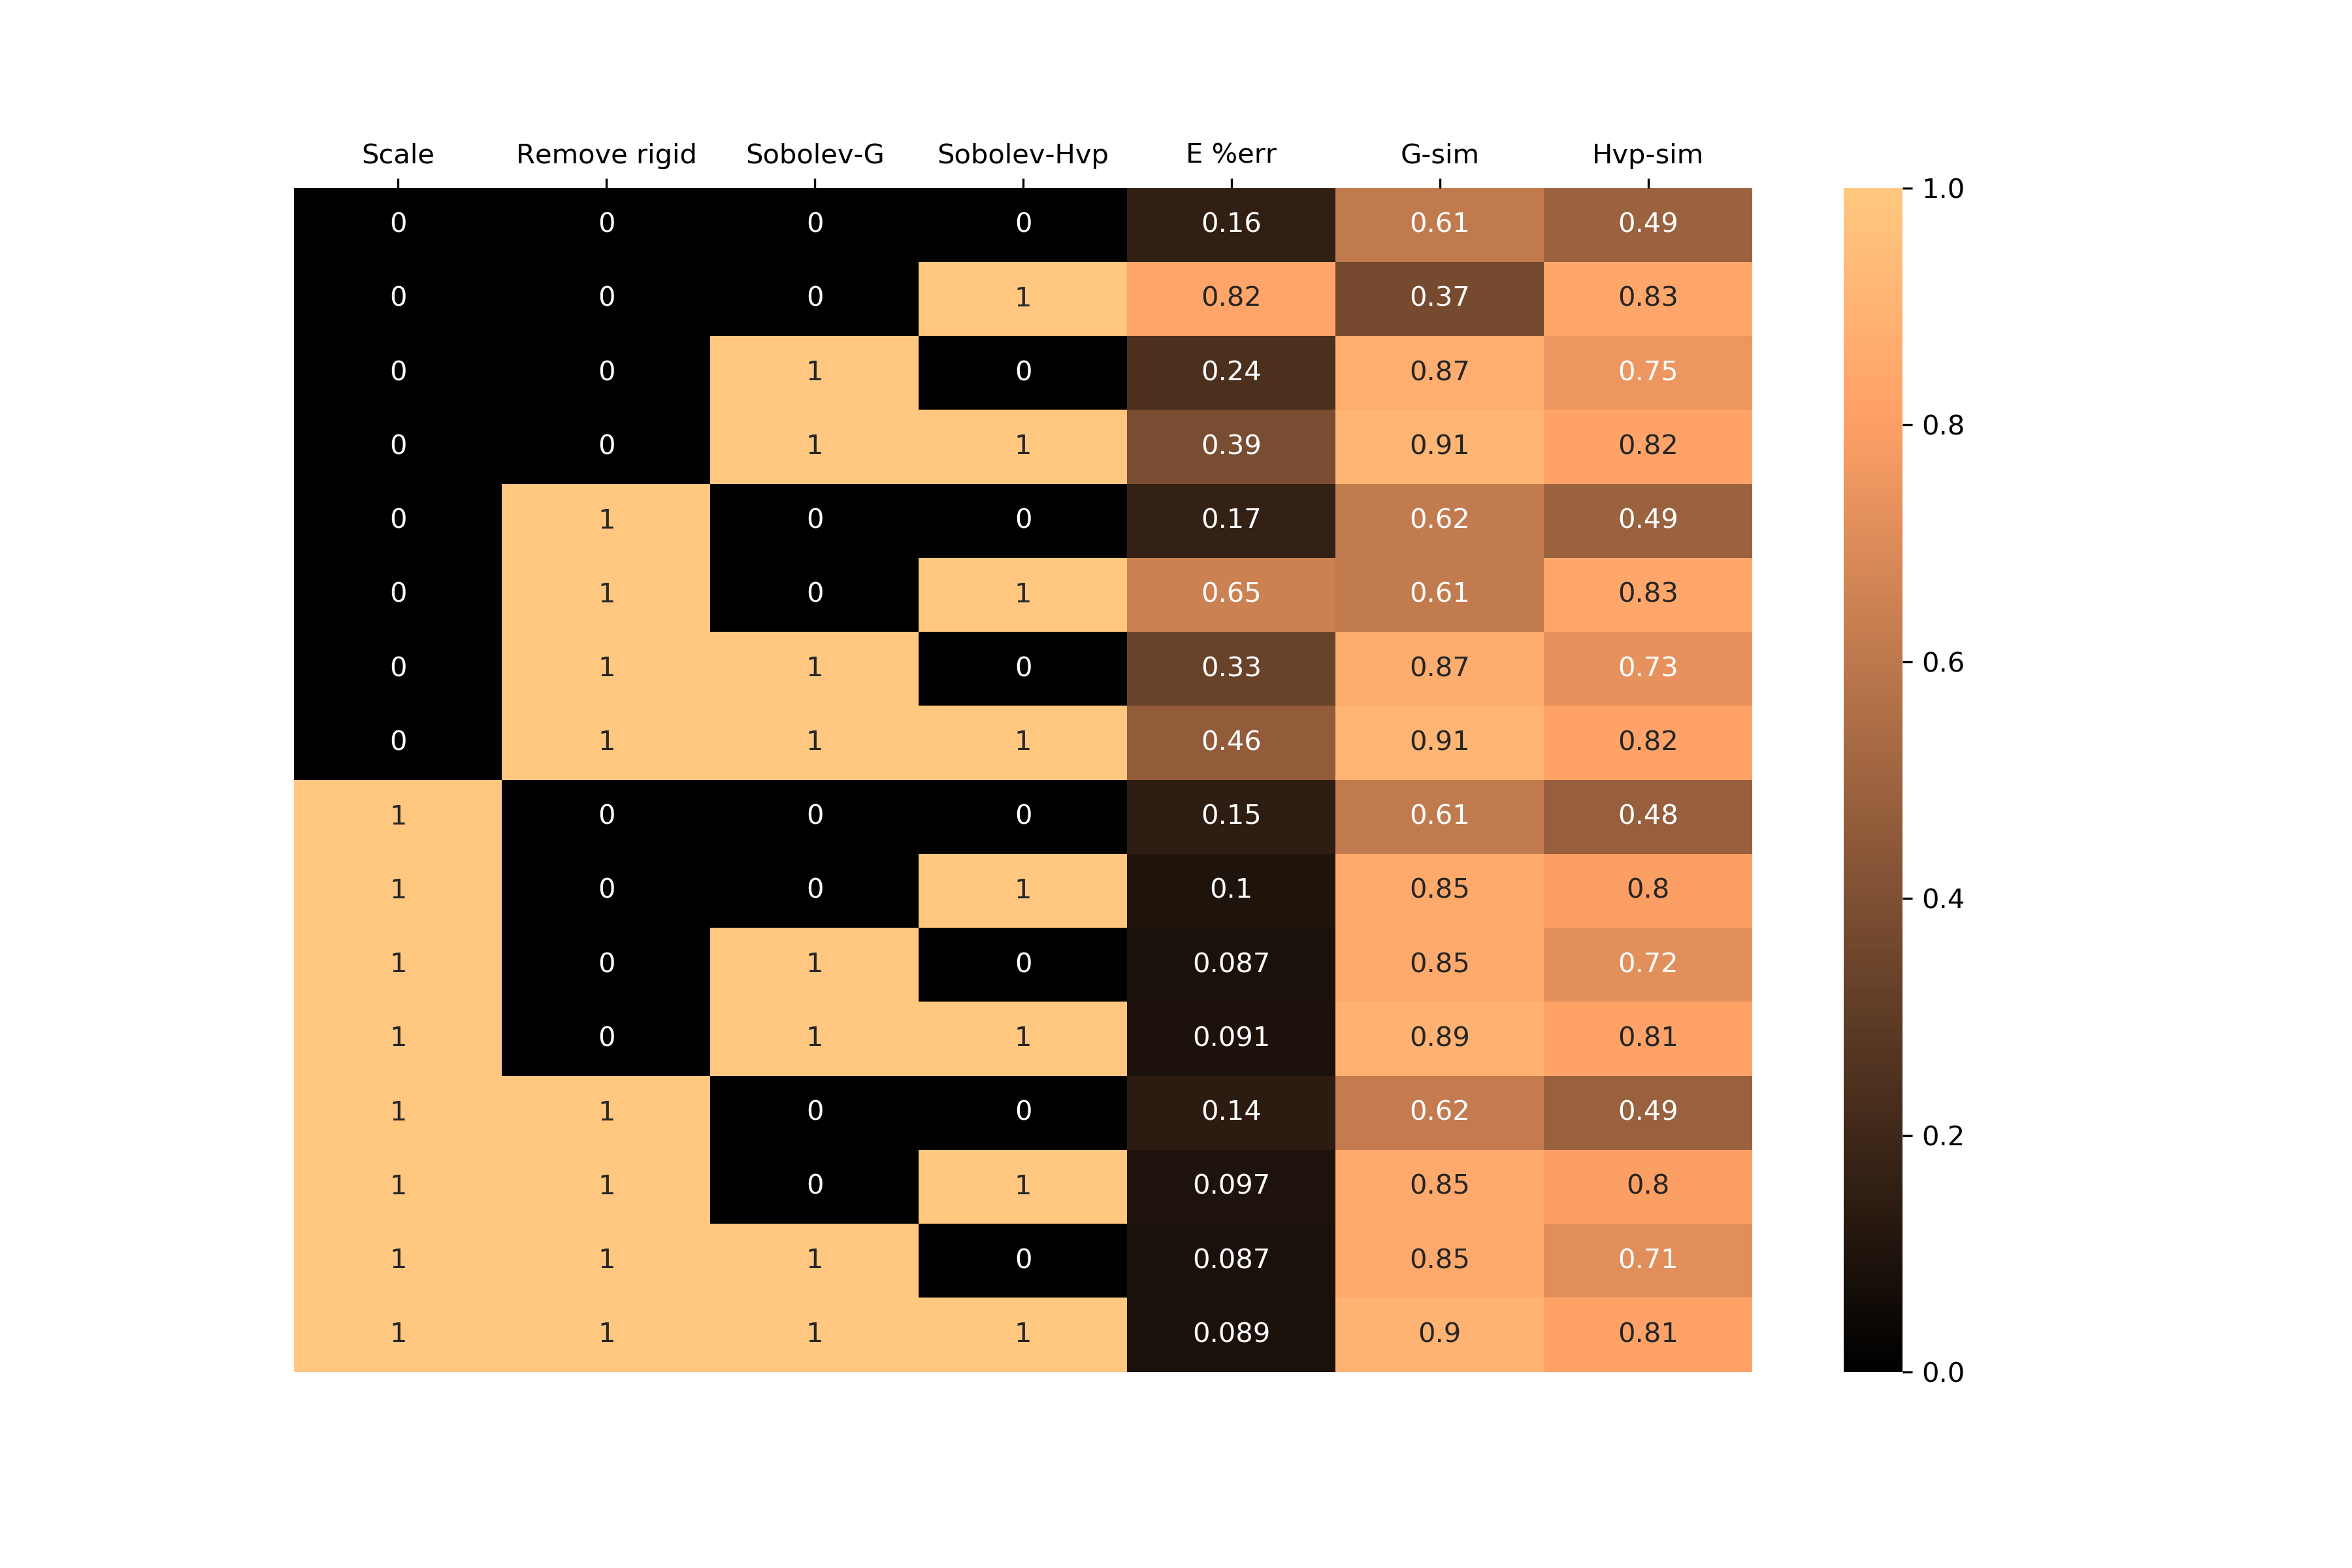
\includegraphics[width=.8\linewidth]{lces/ablation.png}
\end{figure}

\section{Finite element baselines}
We generate meshes for the finite element baselines using two parameters: pore resolution, and minimum mesh resolution.
Firstly, for each pore in the cellular solid, we generate a polygon representing that pore using a number of points equal to pore resolution.
We let the material domain be the overall volume of the solid with these polygons subtracted.
Next, we generate a mesh over the material domain using \textsc{mshr}'s automated mesh generation routine,
passing as resolution minimum mesh resolution multiplied by the number of cells.
In \textsc{mshr}, the resolution parameter controls the maximum cell size, which
is the diameter of the domain's bounding circle divided by the resolution.
It should be noted that cells can be much smaller than this maximum size, or there
can be many more cells than the resolution parameter would imply, as \textsc{mshr}
will place one cell vertex on each point used to construct the domain geometry (i.e. each point in the pore polygon).

\section{Benchmark visualizations}
In the following pages we visualize the solutions found for each pore by each FEA mesh and by CES.
For each pore we use six different finite element meshes.
These respectively used $[4, 8, 16, 32, 48, 64]$ points used to define the geometry of each pore, and minimum of $[1, 2, 4, 8, 12, 16]$ internal mesh vertices along a given axis per pore.
Given these parameters and the geometry of the material domain, meshes were created using the automatic mesh generation tool from mshr (the mesh generation component of FEniCS).
We include the number of degrees of freedom in the finite element basis in each plot.
We superimpose the solution found with CES in red dots on the solution found with FEA.
The CES solution has 690 degrees of freedom in all cases.


\subsection{Compression}
\begin{figure}[H]
\begin{subfigure}{.45\textwidth}
  \centering
  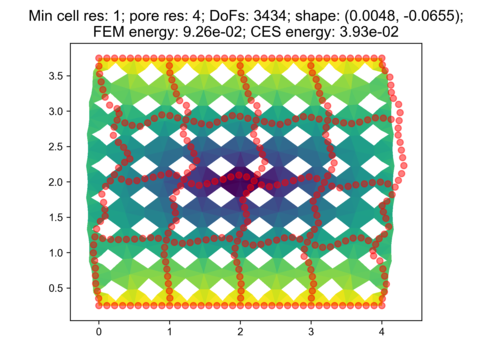
\includegraphics[width=.8\linewidth]{lces/vis_compression/bm_0_mesh_0.png}
\end{subfigure}
\begin{subfigure}{.45\textwidth}
  \centering
  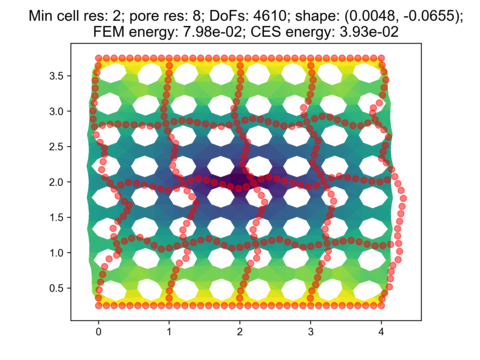
\includegraphics[width=.8\linewidth]{lces/vis_compression/bm_0_mesh_1.png}
\end{subfigure}
\newline
\begin{subfigure}{.45\textwidth}
  \centering
  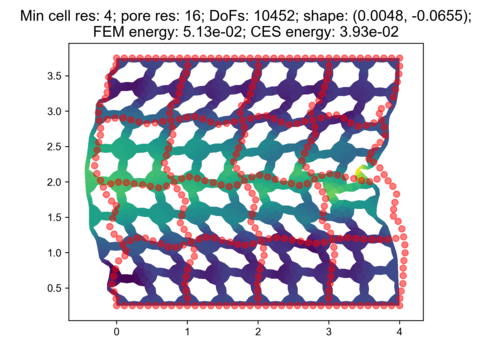
\includegraphics[width=.8\linewidth]{lces/vis_compression/bm_0_mesh_2.png}
\end{subfigure}
\begin{subfigure}{.45\textwidth}
  \centering
  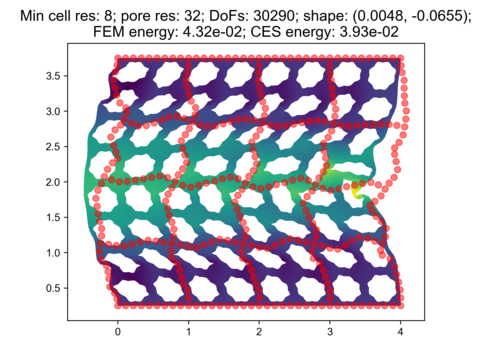
\includegraphics[width=.8\linewidth]{lces/vis_compression/bm_0_mesh_3.png}
\end{subfigure}
\newline
\begin{subfigure}{.45\textwidth}
  \centering
  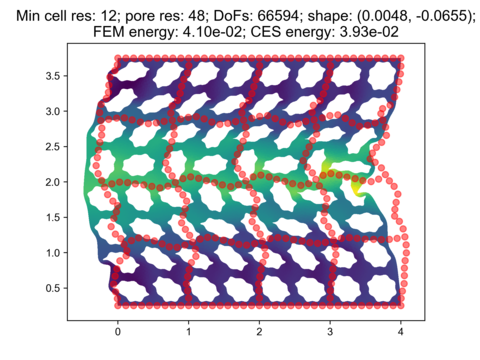
\includegraphics[width=.8\linewidth]{lces/vis_compression/bm_0_mesh_4.png}
\end{subfigure}
\begin{subfigure}{.45\textwidth}
  \centering
  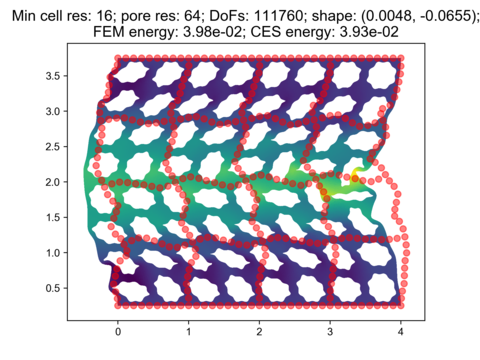
\includegraphics[width=.8\linewidth]{lces/vis_compression/bm_0_mesh_5.png}
\end{subfigure}
\end{figure}

\begin{figure}[H]
\begin{subfigure}{.45\textwidth}
  \centering
  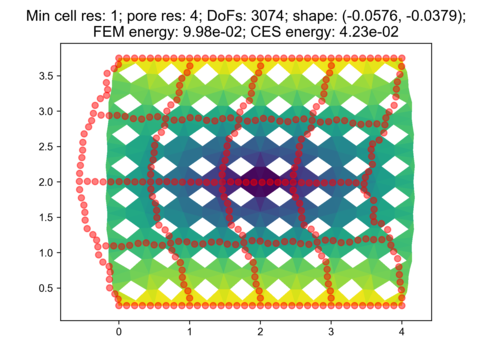
\includegraphics[width=.8\linewidth]{lces/vis_compression/bm_1_mesh_0.png}
\end{subfigure}
\begin{subfigure}{.45\textwidth}
  \centering
  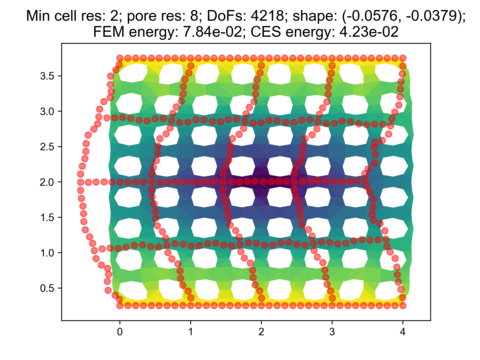
\includegraphics[width=.8\linewidth]{lces/vis_compression/bm_1_mesh_1.png}
\end{subfigure}
\newline
\begin{subfigure}{.45\textwidth}
  \centering
  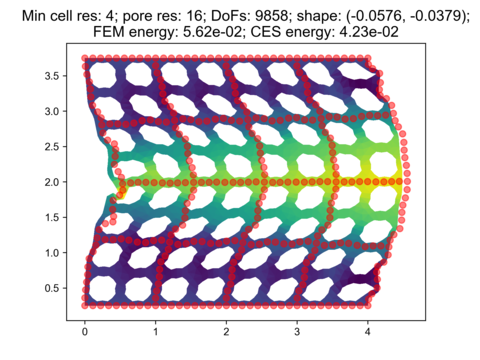
\includegraphics[width=.8\linewidth]{lces/vis_compression/bm_1_mesh_2.png}
\end{subfigure}
\begin{subfigure}{.45\textwidth}
  \centering
  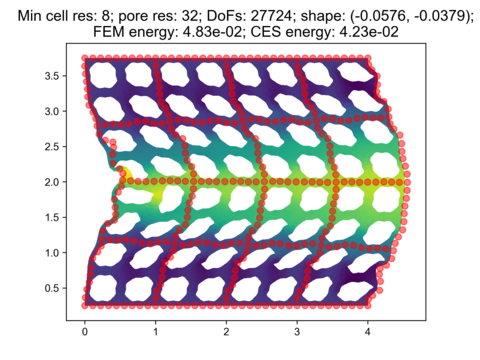
\includegraphics[width=.8\linewidth]{lces/vis_compression/bm_1_mesh_3.png}
\end{subfigure}
\newline
\begin{subfigure}{.45\textwidth}
  \centering
  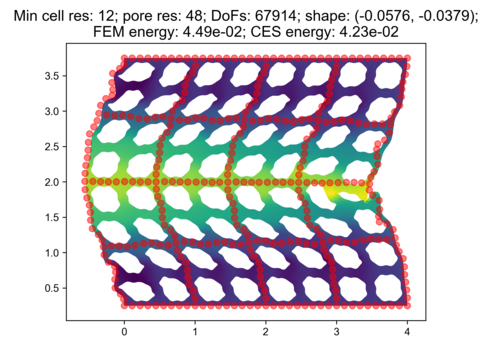
\includegraphics[width=.8\linewidth]{lces/vis_compression/bm_1_mesh_4.png}
\end{subfigure}
\begin{subfigure}{.45\textwidth}
  \centering
  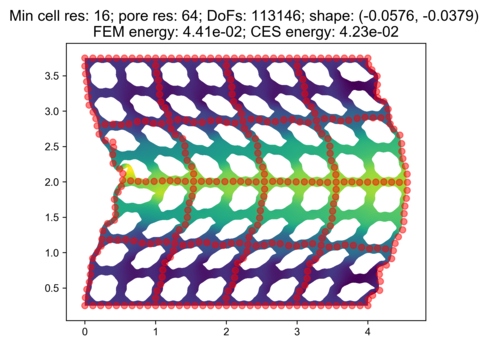
\includegraphics[width=.8\linewidth]{lces/vis_compression/bm_1_mesh_5.png}
\end{subfigure}
\end{figure}

\begin{figure}[H]
\begin{subfigure}{.45\textwidth}
  \centering
  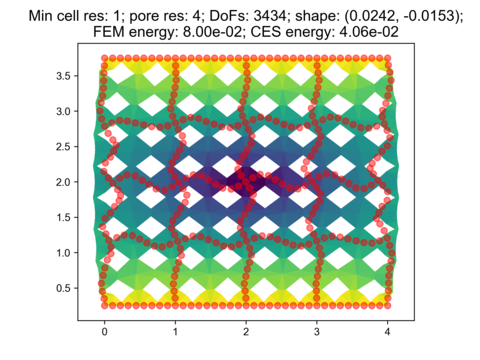
\includegraphics[width=.8\linewidth]{lces/vis_compression/bm_2_mesh_0.png}
\end{subfigure}
\begin{subfigure}{.45\textwidth}
  \centering
  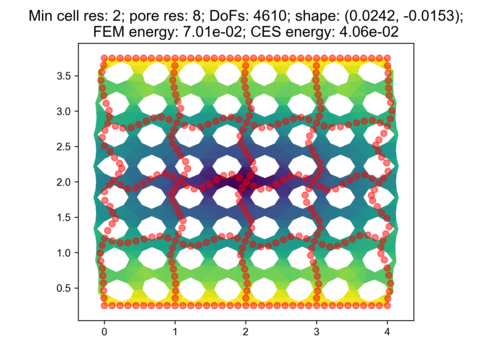
\includegraphics[width=.8\linewidth]{lces/vis_compression/bm_2_mesh_1.png}
\end{subfigure}
\newline
\begin{subfigure}{.45\textwidth}
  \centering
  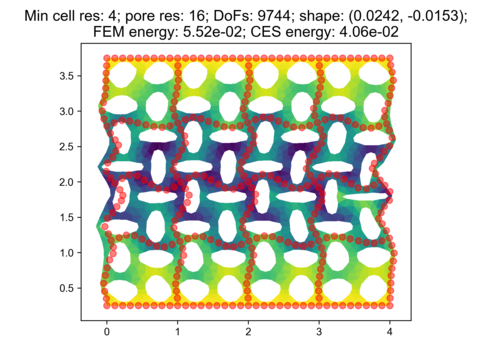
\includegraphics[width=.8\linewidth]{lces/vis_compression/bm_2_mesh_2.png}
\end{subfigure}
\begin{subfigure}{.45\textwidth}
  \centering
  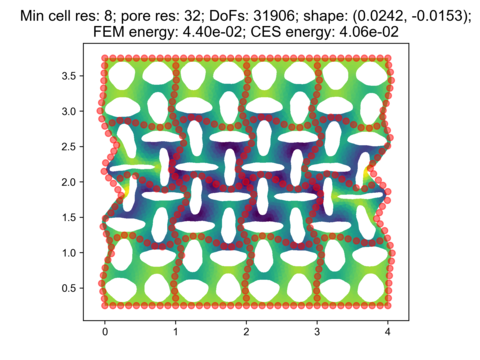
\includegraphics[width=.8\linewidth]{lces/vis_compression/bm_2_mesh_3.png}
\end{subfigure}
\newline
\begin{subfigure}{.45\textwidth}
  \centering
  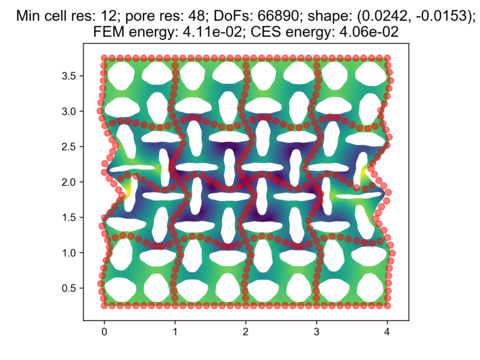
\includegraphics[width=.8\linewidth]{lces/vis_compression/bm_2_mesh_4.png}
\end{subfigure}
\begin{subfigure}{.45\textwidth}
  \centering
  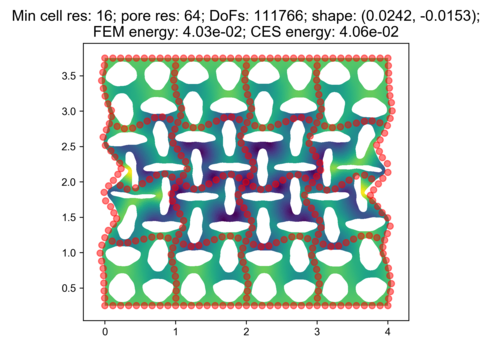
\includegraphics[width=.8\linewidth]{lces/vis_compression/bm_2_mesh_5.png}
\end{subfigure}
\end{figure}

\begin{figure}[H]
\begin{subfigure}{.45\textwidth}
  \centering
  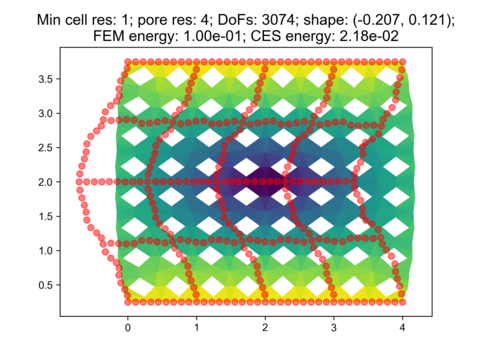
\includegraphics[width=.8\linewidth]{lces/vis_compression/bm_3_mesh_0.png}
\end{subfigure}
\begin{subfigure}{.45\textwidth}
  \centering
  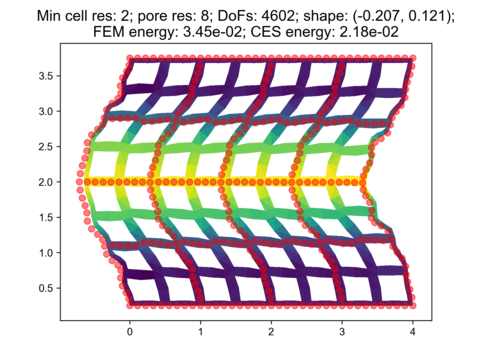
\includegraphics[width=.8\linewidth]{lces/vis_compression/bm_3_mesh_1.png}
\end{subfigure}
\newline
\begin{subfigure}{.45\textwidth}
  \centering
  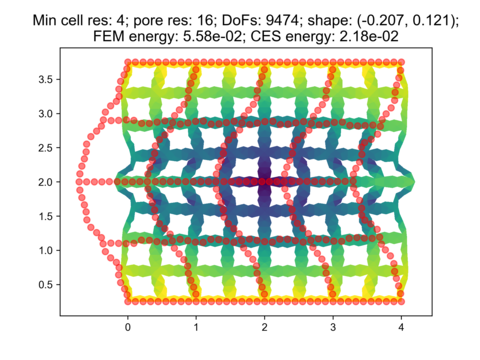
\includegraphics[width=.8\linewidth]{lces/vis_compression/bm_3_mesh_2.png}
\end{subfigure}
\begin{subfigure}{.45\textwidth}
  \centering
  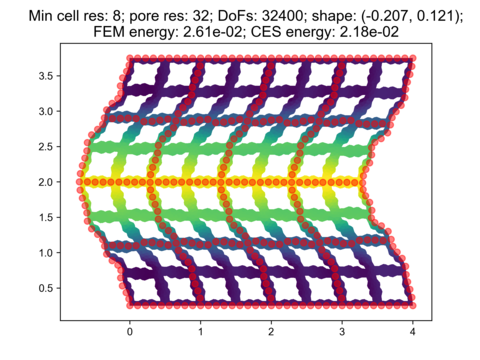
\includegraphics[width=.8\linewidth]{lces/vis_compression/bm_3_mesh_3.png}
\end{subfigure}
\newline
\begin{subfigure}{.45\textwidth}
  \centering
  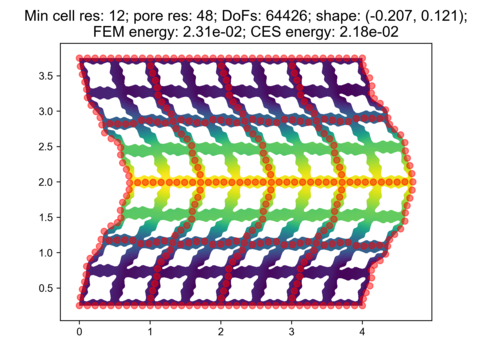
\includegraphics[width=.8\linewidth]{lces/vis_compression/bm_3_mesh_4.png}
\end{subfigure}
\begin{subfigure}{.45\textwidth}
  \centering
  \includegraphics[width=.8\linewidth]{lces/vis_compression/bm_3_mesh_5.png}
\end{subfigure}
\end{figure}

\begin{figure}[H]
\begin{subfigure}{.45\textwidth}
  \centering
  \includegraphics[width=.8\linewidth]{lces/vis_compression/bm_4_mesh_0.png}
\end{subfigure}
\begin{subfigure}{.45\textwidth}
  \centering
  \includegraphics[width=.8\linewidth]{lces/vis_compression/bm_4_mesh_1.png}
\end{subfigure}
\newline
\begin{subfigure}{.45\textwidth}
  \centering
  \includegraphics[width=.8\linewidth]{lces/vis_compression/bm_4_mesh_2.png}
\end{subfigure}
\begin{subfigure}{.45\textwidth}
  \centering
  \includegraphics[width=.8\linewidth]{lces/vis_compression/bm_4_mesh_3.png}
\end{subfigure}
\newline
\begin{subfigure}{.45\textwidth}
  \centering
  \includegraphics[width=.8\linewidth]{lces/vis_compression/bm_4_mesh_4.png}
\end{subfigure}
\begin{subfigure}{.45\textwidth}
  \centering
  \includegraphics[width=.8\linewidth]{lces/vis_compression/bm_4_mesh_5.png}
\end{subfigure}
\end{figure}

\begin{figure}[H]
\begin{subfigure}{.45\textwidth}
  \centering
  \includegraphics[width=.8\linewidth]{lces/vis_compression/bm_5_mesh_0.png}
\end{subfigure}
\begin{subfigure}{.45\textwidth}
  \centering
  \includegraphics[width=.8\linewidth]{lces/vis_compression/bm_5_mesh_1.png}
\end{subfigure}
\newline
\begin{subfigure}{.45\textwidth}
  \centering
  \includegraphics[width=.8\linewidth]{lces/vis_compression/bm_5_mesh_2.png}
\end{subfigure}
\begin{subfigure}{.45\textwidth}
  \centering
  \includegraphics[width=.8\linewidth]{lces/vis_compression/bm_5_mesh_3.png}
\end{subfigure}
\newline
\begin{subfigure}{.45\textwidth}
  \centering
  \includegraphics[width=.8\linewidth]{lces/vis_compression/bm_5_mesh_4.png}
\end{subfigure}
\begin{subfigure}{.45\textwidth}
  \centering
  \includegraphics[width=.8\linewidth]{lces/vis_compression/bm_5_mesh_5.png}
\end{subfigure}
\end{figure}

\begin{figure}[H]
\begin{subfigure}{.45\textwidth}
  \centering
  \includegraphics[width=.8\linewidth]{lces/vis_compression/bm_6_mesh_0.png}
\end{subfigure}
\begin{subfigure}{.45\textwidth}
  \centering
  \includegraphics[width=.8\linewidth]{lces/vis_compression/bm_6_mesh_1.png}
\end{subfigure}
\newline
\begin{subfigure}{.45\textwidth}
  \centering
  \includegraphics[width=.8\linewidth]{lces/vis_compression/bm_6_mesh_2.png}
\end{subfigure}
\begin{subfigure}{.45\textwidth}
  \centering
  \includegraphics[width=.8\linewidth]{lces/vis_compression/bm_6_mesh_3.png}
\end{subfigure}
\newline
\begin{subfigure}{.45\textwidth}
  \centering
  \includegraphics[width=.8\linewidth]{lces/vis_compression/bm_6_mesh_4.png}
\end{subfigure}
\begin{subfigure}{.45\textwidth}
  \centering
  \includegraphics[width=.8\linewidth]{lces/vis_compression/bm_6_mesh_5.png}
\end{subfigure}
\end{figure}

\clearpage

\subsection{Tension}

\begin{figure}[H]
\begin{subfigure}{.45\textwidth}
  \centering
  \includegraphics[width=.8\linewidth]{lces/vis_tension/bm_0_mesh_0.png}
\end{subfigure}
\begin{subfigure}{.45\textwidth}
  \centering
  \includegraphics[width=.8\linewidth]{lces/vis_tension/bm_0_mesh_1.png}
\end{subfigure}
\newline
\begin{subfigure}{.45\textwidth}
  \centering
  \includegraphics[width=.8\linewidth]{lces/vis_tension/bm_0_mesh_2.png}
\end{subfigure}
\begin{subfigure}{.45\textwidth}
  \centering
  \includegraphics[width=.8\linewidth]{lces/vis_tension/bm_0_mesh_3.png}
\end{subfigure}
\newline
\begin{subfigure}{.45\textwidth}
  \centering
  \includegraphics[width=.8\linewidth]{lces/vis_tension/bm_0_mesh_4.png}
\end{subfigure}
\begin{subfigure}{.45\textwidth}
  \centering
  \includegraphics[width=.8\linewidth]{lces/vis_tension/bm_0_mesh_5.png}
\end{subfigure}
\end{figure}

\begin{figure}[H]
\begin{subfigure}{.45\textwidth}
  \centering
  \includegraphics[width=.8\linewidth]{lces/vis_tension/bm_1_mesh_0.png}
\end{subfigure}
\begin{subfigure}{.45\textwidth}
  \centering
  \includegraphics[width=.8\linewidth]{lces/vis_tension/bm_1_mesh_1.png}
\end{subfigure}
\newline
\begin{subfigure}{.45\textwidth}
  \centering
  \includegraphics[width=.8\linewidth]{lces/vis_tension/bm_1_mesh_2.png}
\end{subfigure}
\begin{subfigure}{.45\textwidth}
  \centering
  \includegraphics[width=.8\linewidth]{lces/vis_tension/bm_1_mesh_3.png}
\end{subfigure}
\newline
\begin{subfigure}{.45\textwidth}
  \centering
  \includegraphics[width=.8\linewidth]{lces/vis_tension/bm_1_mesh_4.png}
\end{subfigure}
\begin{subfigure}{.45\textwidth}
  \centering
  \includegraphics[width=.8\linewidth]{lces/vis_tension/bm_1_mesh_5.png}
\end{subfigure}
\end{figure}

\begin{figure}[H]
\begin{subfigure}{.45\textwidth}
  \centering
  \includegraphics[width=.8\linewidth]{lces/vis_tension/bm_2_mesh_0.png}
\end{subfigure}
\begin{subfigure}{.45\textwidth}
  \centering
  \includegraphics[width=.8\linewidth]{lces/vis_tension/bm_2_mesh_1.png}
\end{subfigure}
\newline
\begin{subfigure}{.45\textwidth}
  \centering
  \includegraphics[width=.8\linewidth]{lces/vis_tension/bm_2_mesh_2.png}
\end{subfigure}
\begin{subfigure}{.45\textwidth}
  \centering
  \includegraphics[width=.8\linewidth]{lces/vis_tension/bm_2_mesh_3.png}
\end{subfigure}
\newline
\begin{subfigure}{.45\textwidth}
  \centering
  \includegraphics[width=.8\linewidth]{lces/vis_tension/bm_2_mesh_4.png}
\end{subfigure}
\begin{subfigure}{.45\textwidth}
  \centering
  \includegraphics[width=.8\linewidth]{lces/vis_tension/bm_2_mesh_5.png}
\end{subfigure}
\end{figure}

\begin{figure}[H]
\begin{subfigure}{.45\textwidth}
  \centering
  \includegraphics[width=.8\linewidth]{lces/vis_tension/bm_3_mesh_0.png}
\end{subfigure}
\begin{subfigure}{.45\textwidth}
  \centering
  \includegraphics[width=.8\linewidth]{lces/vis_tension/bm_3_mesh_1.png}
\end{subfigure}
\newline
\begin{subfigure}{.45\textwidth}
  \centering
  \includegraphics[width=.8\linewidth]{lces/vis_tension/bm_3_mesh_2.png}
\end{subfigure}
\begin{subfigure}{.45\textwidth}
  \centering
  \includegraphics[width=.8\linewidth]{lces/vis_tension/bm_3_mesh_3.png}
\end{subfigure}
\newline
\begin{subfigure}{.45\textwidth}
  \centering
  \includegraphics[width=.8\linewidth]{lces/vis_tension/bm_3_mesh_4.png}
\end{subfigure}
\begin{subfigure}{.45\textwidth}
  \centering
  \includegraphics[width=.8\linewidth]{lces/vis_tension/bm_3_mesh_5.png}
\end{subfigure}
\end{figure}

\begin{figure}[H]
\begin{subfigure}{.45\textwidth}
  \centering
  \includegraphics[width=.8\linewidth]{lces/vis_tension/bm_4_mesh_0.png}
\end{subfigure}
\begin{subfigure}{.45\textwidth}
  \centering
  \includegraphics[width=.8\linewidth]{lces/vis_tension/bm_4_mesh_1.png}
\end{subfigure}
\newline
\begin{subfigure}{.45\textwidth}
  \centering
  \includegraphics[width=.8\linewidth]{lces/vis_tension/bm_4_mesh_2.png}
\end{subfigure}
\begin{subfigure}{.45\textwidth}
  \centering
  \includegraphics[width=.8\linewidth]{lces/vis_tension/bm_4_mesh_3.png}
\end{subfigure}
\newline
\begin{subfigure}{.45\textwidth}
  \centering
  \includegraphics[width=.8\linewidth]{lces/vis_tension/bm_4_mesh_4.png}
\end{subfigure}
\begin{subfigure}{.45\textwidth}
  \centering
  \includegraphics[width=.8\linewidth]{lces/vis_tension/bm_4_mesh_5.png}
\end{subfigure}
\end{figure}

\begin{figure}[H]
\begin{subfigure}{.45\textwidth}
  \centering
  \includegraphics[width=.8\linewidth]{lces/vis_tension/bm_5_mesh_0.png}
\end{subfigure}
\begin{subfigure}{.45\textwidth}
  \centering
  \includegraphics[width=.8\linewidth]{lces/vis_tension/bm_5_mesh_1.png}
\end{subfigure}
\newline
\begin{subfigure}{.45\textwidth}
  \centering
  \includegraphics[width=.8\linewidth]{lces/vis_tension/bm_5_mesh_2.png}
\end{subfigure}
\begin{subfigure}{.45\textwidth}
  \centering
  \includegraphics[width=.8\linewidth]{lces/vis_tension/bm_5_mesh_3.png}
\end{subfigure}
\newline
\begin{subfigure}{.45\textwidth}
  \centering
  \includegraphics[width=.8\linewidth]{lces/vis_tension/bm_5_mesh_4.png}
\end{subfigure}
\begin{subfigure}{.45\textwidth}
  \centering
  \includegraphics[width=.8\linewidth]{lces/vis_tension/bm_5_mesh_5.png}
\end{subfigure}
\end{figure}

\begin{figure}[H]
\begin{subfigure}{.45\textwidth}
  \centering
  \includegraphics[width=.8\linewidth]{lces/vis_tension/bm_6_mesh_0.png}
\end{subfigure}
\begin{subfigure}{.45\textwidth}
  \centering
  \includegraphics[width=.8\linewidth]{lces/vis_tension/bm_6_mesh_1.png}
\end{subfigure}
\newline
\begin{subfigure}{.45\textwidth}
  \centering
  \includegraphics[width=.8\linewidth]{lces/vis_tension/bm_6_mesh_2.png}
\end{subfigure}
\begin{subfigure}{.45\textwidth}
  \centering
  \includegraphics[width=.8\linewidth]{lces/vis_tension/bm_6_mesh_3.png}
\end{subfigure}
\newline
\begin{subfigure}{.45\textwidth}
  \centering
  \includegraphics[width=.8\linewidth]{lces/vis_tension/bm_6_mesh_4.png}
\end{subfigure}
\begin{subfigure}{.45\textwidth}
  \centering
  \includegraphics[width=.8\linewidth]{lces/vis_tension/bm_6_mesh_5.png}
\end{subfigure}
\end{figure}


\chapter{Appendix for Chapter 3}
\section{Algorithm pseudocode}
\begin{algorithm}[H]
   \caption{Optimization with randomized telescopes}
   \label{alg:opt}
\begin{algorithmic}
   \STATE {\bfseries Input:} initial parameter $\theta$,
   gradient routine $g(\theta, i)$ which returns $\bar{G}_i(\theta)$,
   compute costs $\bar{C}$,
   exponential decay $\alpha$, tuning frequency $K$, horizon $\bar{H}$,
   reference learning rate $\bar{\eta}$
   \STATE Initialize $B = 0$, next\_tune$ = 0$, $D_{i, j} = 0$
   \REPEAT
   \IF{next\_tune$ <= B$}
   \STATE $\bar{D}, q, W, S \leftarrow \text{tune}(
   \theta, \bar{D}, g, \bar{C}, \alpha, \bar{H})$
   \STATE expectedCompute, expectedSquaredNorm = compute\_and\_variance$(\bar{D}, \bar{C}, S)$
   \STATE $\eta \leftarrow \bar{\eta} \frac{\text{expectedSquaredNorm}}{\bar{D}_{0, \bar{H}}}$
   \STATE $B += \sum_{i=1}^{\bar{H}} \bar{C}({\bar{H}})$
   \STATE next\_tune $+= \bar{C}({\bar{H}})$
   \ENDIF
   \STATE $N \sim q$
   \FOR{$n=1$ {\bfseries to} $N$}
   \STATE $G_n \leftarrow g(\theta, S[n])$
   \ENDFOR
   \STATE $\hat{G} \leftarrow \sum_{n=1}^N G_n W(n, N)$
   \STATE $\theta \leftarrow \theta - \eta \hat{G}$
   \IF{compute reused}
   \STATE $B += \bar{C}({S[N]})$
   \ELSE
   \STATE $B += \sum_{n=1}^N \bar{C}({S[n]})$
   \ENDIF
   \UNTIL{converged}
\end{algorithmic}
\end{algorithm}


\begin{algorithm}[H]
   \caption{tune}
   \label{alg:tune}
\begin{algorithmic}
   \STATE {\bfseries Input:} current parameter $\theta$,
   current squared distance estimates $\bar{D}_{i,j}$,
   gradient routine $g(\theta, i)$ which returns $\bar{G}_i(\theta)$,
   compute costs $\bar{C}$,
   exponential decay $\alpha$, horizon $\bar{H}$
   \STATE $\bar{G}_0(\theta) \leftarrow 0$
   \FOR{$i=1$ {\bfseries to} $\bar{H}$}
   \STATE $\bar{G}_i(\theta) \leftarrow g(\theta, i)$
   \ENDFOR
   \FOR{$i=0$ {\bfseries to} $\bar{H}$}
   \FOR{$j=1$ {\bfseries to} $\bar{H}$}
   \STATE $D_{i, j} \leftarrow ||G_i - G_j||_2^2$
   \ENDFOR
   \ENDFOR
   \STATE $\bar{D} \leftarrow \alpha \bar{D} + (1 - \alpha) D$
   \STATE $S \leftarrow \text{greedy\_subsequence\_select}(\bar{D}, \bar{C})$
   \STATE $q, W \leftarrow \text{$q$\_and\_$W$}(\bar{D}, \bar{C}, S)$
   \STATE {\bfseries Return:} updated estimates $\bar{D}_{i,j}$,
   sampling distribution $q$, weight function $W$, and subsequence $S$
\end{algorithmic}
\end{algorithm}


\begin{algorithm}[H]
   \caption{greedy\_subsequence\_select}
   \label{alg:greedy}
\begin{algorithmic}
   \STATE {\bfseries Input:} Norm estimates $\bar{D}$, compute costs $\bar{C}$
   \STATE Initialize $N = \text{len}(C)$
   \STATE Initialize $S^+ = [N]$, $S^{-} = [1, ..., N]$,
   converged$ = $FALSE, bestAddCost$ = $cost$(\bar{D}, S^+, \bar{C})$,
   bestRemoveCost$ = $cost$(\bar{D}, S^-, \bar{C})$
   \WHILE{not converged}
   \STATE
   \FOR{$i \in [i $ for $ i \in [1 ... N]$ if not $i \in S^+]$}
   \STATE trial$S \leftarrow $sort$(S^+ + [i])$
   \STATE trialCost$ \leftarrow $cost$(\bar{D}, \bar{C}, $trial$S)$
   \IF{trialCost < bestAddCost}
   \STATE $S^+ \leftarrow $trial$S$
   \STATE bestAddCost$ \leftarrow $trialCost
   \STATE converged $\leftarrow$ False
   \STATE BREAK
   \ELSE
   \STATE converged $\leftarrow$ True
   \ENDIF
   \ENDFOR
   \ENDWHILE
   \STATE converged $\leftarrow$ False
   \WHILE{not converged}
   \FOR{$i \in [i $ for $ i \in S^- $ if$ i \neq N$}
   \STATE trial$S \leftarrow [j $ for $ j \in S^- $if$ j != i]$
   \STATE trialCost$ \leftarrow $sequence\_cost$(\bar{D}, C, trial$S$)$
   \IF{trialCost $<$ bestRemoveCost}
   \STATE $S^- \leftarrow $trial$S$
   \STATE bestRemoveCost$ \leftarrow $trialCost
   \STATE converged $\leftarrow$ False
   \STATE BREAK
   \ELSE
   \STATE converged $\leftarrow$ True
   \ENDIF
   \ENDFOR
   \ENDWHILE
   \IF{bestRemoveCost$ > $ bestAddCost}
   \STATE {\bfseries Return:} $S^-$
   \ELSE
   \STATE {\bfseries Return:} $S^+$
   \ENDIF
\end{algorithmic}
\end{algorithm}

\begin{algorithm}[H]
   \caption{compute\_and\_variance}
   \label{alg:cv}
\begin{algorithmic}
   \STATE {\bfseries Input:} Norm estimates $\bar{D}$, compute costs $\bar{C}$, sequence $S$
   \STATE $q$, $W$ $\leftarrow q$\_and\_$W(\bar{D}, \bar{C}, S)$
   \STATE expectedCompute $\leftarrow \sum_{i \in [1 ... |S|]} q(S[i]]) \bar{C}(S[i])$
   \IF{RT-SS}
   \STATE expectedSquaredNorm $\leftarrow \sum_{i \in [1 ... |S|]} q(S[i]]) W(S[i], S[i]) \bar{D}_{S[i-1], S[i]}$
   \ELSIF{RT-RR}
   \STATE expectedSquaredNorm $\leftarrow \sum_{i \in [1 ... |S|]} \sum_{j \in [1 ... i]} q(S[i]]) W(S[j], S[i]) \bar{D}_{S[j], S[i]}$
   \ELSE
   \STATE Undefined: must specify RT-SS or RT-RR
   \ENDIF
   \STATE {\bfseries Return:} expectedCompute, expectedSquaredNorm
\end{algorithmic}
\end{algorithm}

\begin{algorithm}[H]
   \caption{sequence\_cost}
   \label{alg:cost}
\begin{algorithmic}
   \STATE {\bfseries Input:} Norm estimates $\bar{D}$, compute costs $\bar{C}$, sequence $S$
   \STATE expectedCompute, expectedSquaredNorm = compute\_and\_variance$(\bar{D}, \bar{C}, S)$
   \STATE {\bfseries Return:} expectedCompute * expectedSquaredNorm
\end{algorithmic}
\end{algorithm}


\begin{algorithm}[H]
   \caption{$q$\_and\_$W$}
   \label{alg:qandw}
\begin{algorithmic}
   \STATE {\bfseries Input:} $\bar{D}$, $\bar{C}$, and $S$
   \IF{RT-SS}
   \STATE $q(N) \leftarrow \sqrt{\frac{\bar{D}_{S[N], S[N-1]}}{\bar{C}(S[n])}}$
   \STATE $W(n, N) \leftarrow \frac{1}{q(N)} \mathds{1}\{n=N\}$
   \ELSIF{RT-RR}
   \STATE $\tilde{Q}(N) \leftarrow \sqrt{\frac{\bar{D}_{S[N], S[N-1]}}{\bar{C}(S[n]) - \bar{C}(S[n-1])}}$
   \STATE $\tilde(q)(N) \leftarrow $max$(0, \tilde{Q}(N) - \tilde{Q}(N-1))$
   \STATE $q(N) \leftarrow \frac{\tilde{q}(N)}{\sum_i \tilde{q}(i)}$
   \STATE $W(n, N) \leftarrow \frac{1}{1 - \sum_i q(i)} \mathds{1}\{n \leq N\}$
   \ELSE
   \STATE Undefined: must specify RT-SS or RT-RR
   \ENDIF
   \STATE {\bfseries Return:} $q$, $W$
\end{algorithmic}
\end{algorithm}
\clearpage
\section{Proofs}

\subsection{Proofs for section 2}
\subsubsection{Proposition \ref{prop:unbiased}}
\textbf{Unbiasedness of RT estimators.}
The RT estimators in (\ref{eq:rt_general}) are unbiased estimators of
$Y_H$ as long as
\begin{align*}
\mathbb{E}_{N\sim q} [W(n, N) \mathds{1}\{N \geq n\}] = \sum_{N=n}^H W(n, N)q(N) = 1 \quad \forall n\,.
\end{align*}

\begin{proof}
A randomized telescope estimator which satisfies the above linear constraint condition has expectation:
\begin{align*}
\mathbb{E} [\hat{Y}_H] &= \sum_{N=1}^H q(N) \sum_{n=1}^N W(n, N) \Delta_n\\
&= \sum_{n=1}^H \sum_{N=1}^H \Delta_n W(n, N) q(N)\mathds{1}\{n \leq N\}\\
&= \sum_{n=1}^H \Delta_n \sum_{N=n}^H W(n, N) q(N) = \sum_{n=1}^H \Delta_n = Y_H
\end{align*}
\end{proof}

\subsection{Proofs for section 4}

\subsubsection{Theorem \ref{thm:poly}}
\textbf{Bounded variance and compute with polynomial convergence of $\psi$}.
Assume~$\psi$ converges according to~$\psi_n \leq \frac{c}{(n)^p}$ or faster, for constants ${p > 0}$ and~$c > 0$.
Choose the RT-SS estimator with ${q(n) \propto 1/((n)^{p + 1/2})}$.
The resulting estimator~$\hat{G}$ achieves expected compute~${C \leq (\mathcal{H}_{H}^{p-\frac{1}{2}})^2}$, where~$\mathcal{H}_H^i$ is the~$H$th generalized harmonic number of order~$i$, and expected squared norm~${\mathbb{E}[ ||\hat{G}||_2^2 ] \leq c_{\psi}^2 (\mathcal{H}_H^{p-\frac{1}{2}})^2 := \tilde{G}^2}$.
The limit~${\lim_{H \to \infty} \mathcal{H}_H^{p - \frac{1}{2}}}$ is finite iff~${p > \frac{3}{2}}$, in which case it is given by the Riemannian zeta function,~${\lim_{H \to \infty} \mathcal{H}_H^{p - \frac{1}{2}} = \zeta(p - \frac{1}{2})}$.
Accordingly, the estimator achieves horizon-agnostic variance and expected compute bounds iff~${p > \frac{3}{2}}$.
\begin{proof}
Begin by noting the RT-SS estimator returns $\frac{\Delta_n}{q_n}$ with probability $q(n)$.
Let $\bar{q}(n) = \frac{1}{n^{p + \frac{1}{2}}}$ and
$\sum_{n=1}^H \bar{q}(n) = Z$, such that
$q(n) = \frac{\bar{q}(n)}{Z}$. First, note
$Z = \sum_{n=1}^H \frac{1}{n^{p+\frac{1}{2}}} = \text{H}_{H}^{p+\frac{1}{2}}$.
Now inspect the expected squared norm
$\mathbb{E}||\hat{G}||_2^2$:
\begin{align*}
\sum_{n=1}^H q(n) ||\frac{\Delta_n}{q_n}||_2^2 &=
\sum_{n=1}^H q(n) \frac{||\Delta_n||_2^2}{q_n^2} \\
&= Z \sum_{n=1}^H \bar{q}(n) \frac{||\Delta_n||_2^2}{\bar{q}_n^2}\\
&\leq Z c_\psi^2 \sum_{n=1}^H \bar{q}(n) \frac{n^{2p+1}}{n^{2p}}\\
&= Z c_\psi^2 \sum_{n=1}^H \frac{n^{2p+1}}{n^{3p+\frac{1}{2}}}\\
&= Z c_\psi^2 \sum_{n=1}^H \frac{1}{n^{p-\frac{1}{2}}}\\
&= Z c_\psi^2 \text{H}_H^{p-\frac{1}{2}}\\
&= c_\psi^2 \text{H}_H^{p-\frac{1}{2}} \text{H}_H^{p+\frac{1}{2}}\\
&\leq c_\psi^2 (\text{H}_H^{p-\frac{1}{2}})^2
\end{align*}
Now inspect the expected compute, $\mathbb{E}_{n\sim q} n$:
\begin{align*}
\mathbb{E}_{n\sim q} &= \sum_{n=1}^N q(n) n\\
&= Z \sum_{n=1}^H \frac{n}{n^{p+\frac{1}{2}}}\\
&= Z \sum_{n=1}^H \frac{1}{n^{p-\frac{1}{2}}}\\
&= Z \text{H}_H^{p-\frac{1}{2}}\\
&= \text{H}_H^{p-\frac{1}{2}} \text{H}_H^{p+\frac{1}{2}}\\
&\leq (\text{H}_H^{p-\frac{1}{2}})^2
\end{align*}
\end{proof}

\subsubsection{Theorem \ref{thm:geom}}
\textbf{Bounded variance and compute with geometric convergence of $\psi$}.
Assume~$\psi_n$ converges according to~${\psi_n \leq c p^n}$, or faster, for~${0 < p < 1}$.
Choose RT-SS and with~${q(n) \propto p^n}$.
The resulting estimator ~$\hat{G}$ achieves expected compute~${C \leq (1-p)^{-2}}$ and expected squared norm~${||\hat{G}||_2^2 \leq \frac{c}{(1-p)^2} := \tilde{G}^2}$.
Thus, the estimator achieves horizon-agnostic variance and expected compute bounds for all~${0 < p < 1}$.
\begin{proof}
Let $q(n) = \frac{\bar{q}(n)}{Z}$, for $\bar{q}(n) = p^n$.
Note $Z = \sum_{n=1}^H p^n = p \frac{1 - p^H}{1 - p} \leq \frac{1}{1 - p}$.
Now, note $\psi_n = c_\psi \bar{q}(n)$. It follows
\begin{align*}
\mathbb{E}_{n\sim q} ||\frac{\Delta_n}{q(n)}||_2^2
&= \sum_{n=1}^H q(n) \frac{||\Delta_n||_2^2}{q(n)^2} \\
&\leq\sum_{n=1}^H q(n) \frac{\psi_n^2}{q(n)^2} \\
&=\leq c_\psi^2 \sum_{n=1}^H q(n) \frac{\bar{q}(n)^2}{q(n)^2}\\
&= c_\psi^2 Z^2 \sum_{n=1}^H q(n)\\
&= c_\psi^2 Z^2
\end{align*}
Now consider the expected compute. We have
\begin{align*}
\mathbb{E}_{n\sim q} n &= \sum_{n=1}^N n q(n)\\
&= \sum_{n=1}^N \frac{n p^n}{Z}\\
&= \frac{1}{Z} \sum_{n=1}^N n p^n\\
&= p \frac{1}{Z} \frac{1 + Hp^{H+1} - (H+1)p^H}{(1-p)^2}\\
&= \frac{1 + Hp^{H+1} - (H+1)p^H}{(1-p)(1-p^H)}\\
&\leq \frac{1}{(1-p)(1-p^H)}\\
&\leq \frac{1}{(1-p)^2}
\end{align*}
\end{proof}

\subsubsection{Theorem \ref{thm:infopt}}
\textbf{Asymptotic regret bounds for optimizing infinite-horizon programs}.
Assume the setting from \ref{thm:poly} or \ref{thm:geom}, and the corresponding~$C$ and~$\tilde{G}$ from those theorems.
Let~$R_t$ be the instantaneous regret at the~$t$th step of optimization,~${R_t = \mathcal{L}(\theta_t) - \min_\theta \mathcal{L} (\theta)}$.
Let~$t(B)$ be the greatest~$t$ such that a computational budget~$B$ is not exceeded.
Use online gradient descent with step size~${\eta_t = \frac{D}{\sqrt{t} \mathbb{E}[||\hat{G}||_2^2]}}$.
As~${B \to \infty}$, the asymptotic instantaneous regret is bounded by~${R_{t(B)} \leq \mathcal{O} (\tilde{G} D \sqrt{\frac{C}{B}})}$, independent of~$H$.
\begin{proof}
First, we control $t(B)$ using the central limit theorem.
Note $t \to \infty \iff B(t) \to \infty$. Consider $B$ as a function $B(t)$
of $t$. We have $B(t) = \sum_{\tau=1}^t N_t$, where $N \sim q$. Thus,
$\frac{B(t)}{t} \to \mathbb{E}_{N \sim q} N$ by the central limit theorem. This
implies that in the limit, $t = \frac{B}{C}$.

To complete the proof, plug in $t(B)$ and $\eta_t$, as well as the upper bound
on squared norm $\mathbb{E}||\hat{G}||_2^2 \leq \tilde{G}^2$ and upper bound
on diameter $D$, into standard results for stochastic gradient descent with
convex loss functions (e.g. section 3.4 in \cite{hazan2016introduction})
\end{proof}

\subsection{Proofs for section 5}

\subsubsection{Theorem \ref{thm:advcorr-w}}
\textbf{Optimality of RT-SS under adversarial correlation.}
Consider the family of estimators presented in Equation  \ref{eq:rt_general}.
Assume $\theta$, $\nabla_\theta$, and $G$ are univariate.
For any fixed sampling distribution $q$, the single-sample RT estimator RT-SS minimizes the worst-case variance of $\hat{G}$ across an adversarial choice of covariances~${\Cov(\Delta_i, \Delta_j) \leq \sqrt{\Var(\Delta_i)} \sqrt{\Var(\Delta_j)}}$.

\begin{proof}
Recall $\hat{G} = \sum_{n=0}^N \Delta_n W(n, N)$. Let $\sigma_{i, j}^2 = \Cov(\Delta_i, \Delta_j)$ and $\sigma_i^2 = \Var(\Delta_i)$. The variance of $\hat{G}$ is:
\begin{align*}
\Var(\hat{G}) &= \sum_N q(N) \Big[\sum_{i=0}^N \sum_{j=0}^N W(i, N) W(j, N) \sigma_{i, j}^2 \Big] \\
&\leq \sum_N q(N) \Big[\sum_{i=0}^N \sum_{j=0}^N W(i, N) W(j, N) \sigma_i \sigma_j \Big] \\
&= \sum_N q(N) \Big(\sum_{n=0}^N W(n, N) \sigma_n \Big)^2
\end{align*}
Note the above bound is tight as the adversary can choose $\Cov(\Delta_i, \Delta_j) = \sigma_i \sigma_j$. Introduce $\rho(n, N) = W(n, N) q(N)$, and note that the constraint from proposition \ref{prop:unbiased} can equivalently be stated as $\sum_{N \geq n} \rho(n, N) = 1 \forall n$. We have the variance:
\[
\Var(\hat{G} | N) \leq \sum_N \frac{1}{q(N)} \Big(\sum_{n=0}^N \rho(n, N) \sigma_n \Big)^2
\]
Consider finding $\rho(n, N)$ which minimizes the variance for an arbitrary $q$. The constrained optimization has the Lagrangian:
\[
J = \Big(\sum_N \frac{1}{q(N)} (\sum_{n=0}^N \rho(n, N) \sigma_n )^2\Big) + \sum_n \lambda_n (\sum_{N \geq n} \rho(n, N) - 1)
\]
We can accordingly optimize by taking derivatives:
\begin{align*}
    \frac{dJ}{d\rho(n, N)} &= 2C q(N)(\sum_{i=0}^N w(i, N) \sigma_i) \sigma_n + \lambda_n\\
    \frac{dJ}{d\rho(n, N)} = 0 &\implies \sigma_n q(N) \sum_{i=0}^N w(i, N) \sigma_i = k_n\\
    &\implies \sigma_n \sum_{i=0}^N \rho(i, N) \sigma_i = k_n \forall N \geq n\\
    &\implies \rho(n, N) = 0 \forall N > n
\end{align*}
\end{proof}

\subsubsection{Theorem \ref{thm:advcorr-q}}
\textbf{Optimal q under adversarial correlation.}
Consider the family of estimators presented in Equation  \ref{eq:rt_general}.
Assume $\Cov(\Delta_i, \Delta_i)$ and $\Cov(\Delta_i, \Delta_j)$ are diagonal.
The RT-SS estimator with~${q_n \propto \sqrt{\frac{\mathbb{E}[||\Delta_n||_2^2}{C(n)}}}$ maximizes the ROE across an adversarial choice of diagonal covariance matrices~${\Cov(\Delta_i, \Delta_j)_{kk} \leq \sqrt{\Cov(\Delta_i, \Delta_i)_{kk} \Cov(\Delta_j, \Delta_j)_{kk}}}$.
\begin{proof}
First, note that by the assumption of diagonal covariance between all terms,
the expected squared norm decomposes over indices $k$:
\[
\mathbb{E} ||\hat{G}||_2^2 = \sum_k \mathbb{E} \hat{G}[k]^2
\]
For all choices of $q$, the RT-SS estimator minimizes the worst-case variance and thus
(due to unbiasedness) the expected squared value of each entry in $\hat{G}$.
Because the squared norm decomposes, the RT-SS estimator minimizes the squared
norm for all $q$.

It remains to optimize $q$. We know $\rho(n, N) = 0 \forall N > n$.
Therefore to satisfy the constraint, we have $\rho(N, N) = 1$.
It follows that:
\[
\text{ROE}^-1 = \big( \sum_N q(N) C(N) \big) \big(\sum_N \frac{\mathbb{E}||\Delta_N||_2^2}{q(N)} \big)
\]
We require $\sum_N q(N) = 1$. The constrained optimization has the Lagrangian:
\[
J = \Big( \sum_N q(N) C(N) \Big) \Big(\sum_N \frac{\mathbb{E}||\Delta_N||_2^2}{q(N)}\Big) + \lambda (\sum_N q(N) - 1)
\]
Let $C = \Big( \sum_N q(N) C(N) \Big)$ and $V = \Big(\sum_N \frac{\mathbb{E}||\Delta_N||_2^2}{q(N)}\Big)$. We optimize $q(N)$ by taking the derivative of the inverse ROE:
\begin{align*}
\frac{d\text{ROE}^{-1}}{dq(N)} &= C(N) V - C \frac{\sigma_N^2}{q(N)^2}\\
\frac{d\text{ROE}^{-1}}{dq(N)} = 0 &\implies q(N)^2 \propto \frac{\mathbb{E}||\Delta_N||_2^2 C}{C(N) V}\\
&\implies q(N) \propto \sqrt{\frac{\mathbb{E}||\Delta_N||^2_2}{C(N)}}
\end{align*}
\end{proof}

\subsubsection{Theorem \ref{thm:nocorr-w}}
\textbf{Optimality of RT-RR under independence}.
Consider the family of estimators presented in Eq.~\ref{eq:rt_general}.
Assume the $\Delta_j$ are univariate.
When the~$\Delta_j$ are uncorrelated, for any importance sampling distribution~$q$, the Russian roulette estimator achieves the minimum variance in this family and thus maximizes the optimization efficiency lower bound.
\begin{proof}
By independence, we have $\mathbb{E}\big(\sum_n W(n, N) \Delta_n \big)^2 = \sum_n W(n, N)^2 \mathbb{E} \Delta_n^2$. It follows that an RT estimator has variance:
\begin{align*}
\Var(\hat{G}) &= \sum_N q(N) \sum_{n\leq N} W(n, N)^2 \mathbb{E} \Delta_n^2\\
&= \sum_N \frac{1}{q(N)} \sum_{n\leq N} \rho(n, N)^2 \mathbb{E} \Delta_n^2
\end{align*}
Recall the constraint in proposition \ref{prop:unbiased} requires $\sum_{N \geq n} \rho(n, N) = 1$ for all $n$. The Lagrangian of the constrained minimization of $\Var(\hat{G})$ with respect to $\rho$ is:
\[
J = \Var(\hat{G}) + \sum_n \lambda_n (\sum_{N \geq n} \rho_n - 1)
\]
We optimize $\rho$ by finding the minimum of the Lagrangian:
\begin{align*}
\frac{dJ}{d\rho(n,N)} &= \frac{2}{q(N)} \rho(n, N) \mathbb{E} \Delta_n^2 + \lambda_n \\
\frac{dJ}{d\rho(n,N)} = 0 &\implies \frac{\rho(n, N)}{q(N)} = -\frac{\lambda_n}{2 \mathbb{E} \Delta_n^2}\\
&\implies W(n, N) = -\frac{\lambda_n}{2 \mathbb{E} \Delta_n^2}, \text{ which is independent of } N\\
&\implies W(n, N) = \frac{1}{\sum_{N' \geq n} q(N')} \text{ to fulfill the constraint in proposition }\ref{prop:unbiased}
\end{align*}
\end{proof}

\subsubsection{Theorem \ref{thm:nocorr-q}}
\textbf{Optimal q under independence}.
Consider the family of estimators presented in Equation  \ref{eq:rt_general}.
Assume $\Cov(\Delta_i, \Delta_i)$ is diagonal and~$\Delta_i$ and~$\Delta_j$ are independent.
The RT-RR estimator with
$Q(i) \propto \sqrt{\frac{\mathbb{E} [||\Delta_i||_2^2}{C(i) - C(i-1)}]}$,
where $Q(i) = \Pr(n \geq i) = \sum_{j=i}^H q(j)$,
maximizes the ROE.

\begin{proof}
First note that by theorem \ref{thm:nocorr-w}, for any $q$ and for each element in the vector
$\hat{G}$, the RT-RR estimator minimizes the variance of that element. Now note
that due to independence of $\Delta_i, \Delta_j$ and diagonality of $\Cov(\Delta_i, \Delta_i)$:
\begin{align*}
\mathbb{E} ||\sum_{n=1}^N W(n, N) \Delta_n||_2^2 &= \sum_{n=1}^N W(n, N) \mathbb{E} ||\Delta_n||_2^2\\
&= \sum_k \sum_{n=1}^N W(n, N) \mathbb{E}\Delta_n[k]^2
&= \sum_k \mathbb{E} \hat{G}[k]^2
\end{align*}
As the RT-RR estimator minimizes $\mathbb{E} \hat{G}[k]^2$ for each coordinate $k$,
it also minimizes $\mathbb{E} ||\hat{G}||_2^2$. It remains to optimize $Q$.
Consider the inverse ROE of the RT-RR estimator. By independence we have:
\begin{align*}
    \text{ROE}(\hat{G})^{-1} = \mathbb{E} ||\hat{G}||_2^2 \mathbb{E} C &=
    \Big(\sum_N q(N) \sum_{n\leq N} \frac{1}{Q(n)^2} \mathbb{E} ||\Delta_n||_2^2\Big) \Big(\sum_N q(N) C(N)\Big)
\end{align*}
Take the gradient of the inverse optimization efficiency lower bound w.r.t. $q(n)$:
\[
\frac{d\text{ROE}(\hat{G})^{-1}}{dq(N)} = C(N) \mathbb{E} ||\hat{G}||_2^2 + \sum_{n \leq N} \frac{1}{Q(n)^2} \mathbb{E} ||\Delta_n||_2^2 - \sum_{i} q(i) \sum_{j \leq min(i, N)} \frac{2}{Q(j)^3} \mathbb{E} ||\Delta_j||_2^2\\
\]
\begin{align*}
\sum_{i} q(i) \sum_{j \leq min(i, N)} \frac{2}{Q(j)^3} \mathbb{E} ||\Delta_j||_2^2 &= \sum_{j \leq N} \frac{2}{Q(j)^2} \mathbb{E} ||\Delta_j||_2^2 \frac{\sum_i q(i) \mathds{1}\{i \geq j\}}{Q(j)}\\
&= \sum_{j \leq N} \frac{2}{Q(j)^2} \mathbb{E} ||\Delta_j||_2^2 \quad \text{ by definition of } Q(j)
\end{align*}
\[
\implies \frac{d\text{ROE}(\hat{G})^{-1}}{dq(N)} = C(N) \mathbb{E} ||\hat{G}||_2^2 - \sum_{n \leq N} \frac{1}{Q(n)^2} \mathbb{E} ||\Delta_n||_2^2
\]
Now optimize the objective w.r.t. $Q$ by finding the critical point:
\begin{align*}
\frac{d\text{ROE}(\hat{G})^{-1}}{dq(N)} = 0 \implies C(N) \mathbb{E} ||\hat{G}||_2^2 &=  \sum_{n \leq N} \frac{1}{Q(n)^2} \mathbb{E} ||\Delta_n||_2^2\\
\implies \mathbb{E} ||\hat{G}||_2^2 \Big(C(N) - C(N-1)\Big) &= \frac{1}{2}  \frac{\mathbb{E}||\Delta_N||_2^2}{Q(N)^2}\\
\implies Q(N)^2 &\propto \frac{\mathbb{E} ||\Delta_n||_2^2}{C(N) - C(N-1)}
\end{align*}
\end{proof}


\end{document}
